% Options for packages loaded elsewhere
\PassOptionsToPackage{unicode}{hyperref}
\PassOptionsToPackage{hyphens}{url}
%
\documentclass[
  12pt,
]{article}
\usepackage{amsmath,amssymb}
\usepackage{iftex}
\ifPDFTeX
  \usepackage[T1]{fontenc}
  \usepackage[utf8]{inputenc}
  \usepackage{textcomp} % provide euro and other symbols
\else % if luatex or xetex
  \usepackage{unicode-math} % this also loads fontspec
  \defaultfontfeatures{Scale=MatchLowercase}
  \defaultfontfeatures[\rmfamily]{Ligatures=TeX,Scale=1}
\fi
\usepackage{lmodern}
\ifPDFTeX\else
  % xetex/luatex font selection
\fi
% Use upquote if available, for straight quotes in verbatim environments
\IfFileExists{upquote.sty}{\usepackage{upquote}}{}
\IfFileExists{microtype.sty}{% use microtype if available
  \usepackage[]{microtype}
  \UseMicrotypeSet[protrusion]{basicmath} % disable protrusion for tt fonts
}{}
\makeatletter
\@ifundefined{KOMAClassName}{% if non-KOMA class
  \IfFileExists{parskip.sty}{%
    \usepackage{parskip}
  }{% else
    \setlength{\parindent}{0pt}
    \setlength{\parskip}{6pt plus 2pt minus 1pt}}
}{% if KOMA class
  \KOMAoptions{parskip=half}}
\makeatother
\usepackage{xcolor}
\usepackage[margin=1in]{geometry}
\usepackage{graphicx}
\makeatletter
\def\maxwidth{\ifdim\Gin@nat@width>\linewidth\linewidth\else\Gin@nat@width\fi}
\def\maxheight{\ifdim\Gin@nat@height>\textheight\textheight\else\Gin@nat@height\fi}
\makeatother
% Scale images if necessary, so that they will not overflow the page
% margins by default, and it is still possible to overwrite the defaults
% using explicit options in \includegraphics[width, height, ...]{}
\setkeys{Gin}{width=\maxwidth,height=\maxheight,keepaspectratio}
% Set default figure placement to htbp
\makeatletter
\def\fps@figure{htbp}
\makeatother
\setlength{\emergencystretch}{3em} % prevent overfull lines
\providecommand{\tightlist}{%
  \setlength{\itemsep}{0pt}\setlength{\parskip}{0pt}}
\setcounter{secnumdepth}{5}
\usepackage{url}
\usepackage{setspace}
%\singlespacing
%\onehalfspacing
%\doublespacing
\usepackage{lineno}
%\linenumbers
\usepackage[belowskip=0pt,aboveskip=0pt]{caption}
\usepackage{relsize}
\newcommand{\Fmsy}{\ensuremath{F_{\text{MSY}}}\xspace}
\newcommand{\Fspr}[1]{\ensuremath{F_{\text{{#1}\%}}}\xspace}
\newcommand{\afrb}{Alaska Fishery Research Bulletin\xspace}
\newcommand{\ajms}{African Journal of Marine Science\xspace}
\newcommand{\amb}{Advances in Marine Biology\xspace}
\newcommand{\bms}{Bulletin of Marine Science\xspace}
\newcommand{\bjssf}{Bulletin of the Japanese Society of Scientific Fisheries\xspace}
\newcommand{\cb}{Conservation Biology\xspace}
\newcommand{\cjfas}{Canadian Journal of Fisheries and Aquatic Sciences\xspace}
\newcommand{\ea}{Ecological Applications\xspace}
\newcommand{\eer}{Evolutionary Ecology Research\xspace}
\newcommand{\elet}{Ecology Letters\xspace}
\newcommand{\emod}{Ecological Modelling\xspace}
\newcommand{\ebf}{Environmental Biology of Fishes\xspace}
\newcommand{\ff}{Fish and Fisheries\xspace}
\newcommand{\fo}{Fisheries Oceanography\xspace}
\newcommand{\fr}{Fisheries Research\xspace}
\newcommand{\fb}{Fishery Bulletin\xspace}
\newcommand{\ijms}{ICES Journal of Marine Science\xspace}
\newcommand{\iccat}{Collective Volume of Scientific Papers ICCAT\xspace}
\newcommand{\jae}{Journal of Animal Ecology\xspace}
\newcommand{\jai}{Journal of Applied Ichthyology\xspace}
\newcommand{\jdc}{Journal Du Conseil International Pour L'exploration De La Mer\xspace}
\newcommand{\jdcp}{Journal Du Conseil Permanent International Pour L'exploration De La Mer\xspace}
\newcommand{\jembe}{Journal of Experimental Marine Biology and Ecology\xspace}
\newcommand{\jfb}{Journal of Fish Biology\xspace}
\newcommand{\jsr}{Journal of Sea Research\xspace}
\newcommand{\jtb}{Journal of Theoretical Biology\xspace}
\newcommand{\jfrbc}{Journal of the Fisheries Research Board of Canada\xspace}
\newcommand{\jnwafs}{Journal of Northwest Atlantic Fisheries Science\xspace}
\newcommand{\mcf}{Marine and Coastal Fisheries: Dynamics, Management, and Ecosystem Science\xspace}
\newcommand{\mb}{Marine Biology\xspace}
\newcommand{\meps}{Marine Ecology Progress Series\xspace}
\newcommand{\mfr}{Marine Fisheries Review\xspace}
\newcommand{\mpb}{Marine Pollution Bulletin\xspace}
\newcommand{\najfm}{North American Journal of Fisheries Management\xspace}
\newcommand{\nzjmfr}{New Zealand Journal of Marine and Freshwater Research\xspace}
\newcommand{\pnas}{Proceedings of the National Academy of Sciences USA\xspace}
\newcommand{\rpvrciemm}{Rapports et Proc\`es-Verbaux des R\'eunions. Conseil Internationale pour l'Exploration de la Mer\xspace}
\newcommand{\rpvrcpiemm}{Rapports et Proc\`es-Verbaux des R\'eunions. Conseil Permanent Internationale pour l'Exploration de la Mer\xspace}
\newcommand{\rfbf}{Reviews in Fish Biology and Fisheries\xspace}
\newcommand{\sajms}{South African Journal of Marine Science\xspace}
\newcommand{\tafs}{Transactions of the American Fisheries Society\xspace}

\newcommand{\anzjs}{Australian \& New Zealand Journal of Statistics\xspace}
\newcommand{\as}{Applied Statistics\xspace}
\newcommand{\csda}{Computational Statistics \& Data Analysis\xspace}
\newcommand{\ees}{Environmental and Ecological Statistics\xspace}
\newcommand{\jas}{Journal of Applied Statistics\xspace}
\newcommand{\jabes}{Journal of Agricultural, Biological, and Environmental Statistics\xspace}
\newcommand{\jasa}{Journal of the American Statistical Association\xspace}
\newcommand{\jrssb}{Journal of the Royal Statistical Society. Series B\xspace}
\newcommand{\sm}{Statistics in Medicine}

\usepackage{float}
\usepackage{amsmath}
\usepackage{pdflscape}
\usepackage{hyperref}
\usepackage{xspace}
\usepackage{bm}
\usepackage{caption,graphics}
\usepackage{graphicx}
\usepackage{makecell}
\usepackage{lineno}
\linenumbers
\renewcommand\figurename{Fig.}
\captionsetup{labelsep=period, singlelinecheck=false}
\newcommand{\changesize}[1]{\fontsize{#1pt}{#1pt}\selectfont}
\renewcommand{\arraystretch}{1.5}
\renewcommand\theadfont{}
\usepackage{booktabs}
\usepackage{longtable}
\usepackage{array}
\usepackage{multirow}
\usepackage{wrapfig}
\usepackage{float}
\usepackage{colortbl}
\usepackage{pdflscape}
\usepackage{tabu}
\usepackage{threeparttable}
\usepackage{threeparttablex}
\usepackage[normalem]{ulem}
\usepackage{makecell}
\usepackage{xcolor}
\ifLuaTeX
  \usepackage{selnolig}  % disable illegal ligatures
\fi
\usepackage[]{natbib}
\bibliographystyle{cjfas2.bst}
\IfFileExists{bookmark.sty}{\usepackage{bookmark}}{\usepackage{hyperref}}
\IfFileExists{xurl.sty}{\usepackage{xurl}}{} % add URL line breaks if available
\urlstyle{same}
\hypersetup{
  pdftitle={Supplementary files: Evaluating the impact of log-normal bias-correction on a state-space stock assessment model},
  pdfauthor={Chengxue Li\^{}\{1,2,3*\}; Jonathan J. Deroba\^{}1; Timothy J. Miller\^{}1; Christopher M. Legault\^{}1; Charles T. Perretti\^{}1},
  hidelinks,
  pdfcreator={LaTeX via pandoc}}

\title{Supplementary files: Evaluating the impact of log-normal
bias-correction on a state-space stock assessment model}
\author{Chengxue Li\(^{1,2,3*}\) \and Jonathan J.
Deroba\(^1\) \and Timothy J. Miller\(^1\) \and Christopher M.
Legault\(^1\) \and Charles T. Perretti\(^1\)}
\date{}

\begin{document}
\maketitle

\(^1\) Northeast Fisheries Science Center, Woods Hole Laboratory, 166
Water Street, Woods Hole, MA 02543 USA

\(^2\) School of Marine and Atmospheric Sciences, Stony Brook
University, Stony Brook, NY 11794, USA

\(^3\) Saltwater Inc., 733 N Street, Anchorage, AK 99501 USA

\(^*\)Corresponding author:
\href{mailto:chengxue.li@noaa.gov}{\nolinkurl{chengxue.li@noaa.gov}}

\vspace{0.5cm}

\textbf{ORCID:}

Chengxue Li:
\href{https://orcid.org/0000-0001-7518-7234}{0000-0001-7518-7234}

Timothy J. Miller:
\href{https://orcid.org/0000-0003-1411-1206}{0000-0003-1411-1206}

Christopher M. Legault:
\href{https://orcid.org/0000-0002-0328-1376}{0000-0002-0328-1376}

Charles T. Perretti:
\href{https://orcid.org/0000-0002-4316-3630}{0000-0002-4316-3630}.

\pagebreak

\renewcommand{\thetable}{S\arabic{table}}
\setcounter{table}{0}

\begin{table}[H]
    \centering
    \caption{Parameters associated with random effects processes used for Georges Bank (GB) yellowtail flounder.}
    \label{supp_flounder_table}
    \begin{table}[H]
    \centering
    \begin{tabular}{llrll}
        \toprule
        Random Effects Structure & Proc./Obs. & Rec sigma & NAA sigma & Rho (AR1\_y) \\
        \midrule
        Rec (iid)       & ON \& ON   & 1.07 & NA & NA \\
        Rec (iid)       & OFF \& ON  & 1.07 & NA & NA \\
        Rec (iid)       & ON \& OFF  & 1.08 & NA & NA \\
        Rec (iid)       & OFF \& OFF & 1.08 & NA & NA \\
        Rec (ar1\_y)    & ON \& ON   & 0.37 & NA & 0.96 \\
        Rec (ar1\_y)    & OFF \& ON  & 0.37 & NA & 0.96 \\
        Rec (ar1\_y)    & ON \& OFF  & 0.37 & NA & 0.96 \\
        Rec (ar1\_y)    & OFF \& OFF & 0.37 & NA & 0.96 \\
        Rec+NAA (iid)      & ON \& ON   & 1.23 & 0.55 & NA \\
        Rec+NAA (iid)      & OFF \& ON  & 1.23 & 0.56 & NA \\
        Rec+NAA (iid)      & ON \& OFF  & 1.24 & 0.55 & NA \\
        Rec+NAA (iid)      & OFF \& OFF & 1.24 & 0.56 & NA \\
        Rec+NAA (ar1\_y)   & ON \& ON   & 0.55 & 0.21 & 0.94 \\
        Rec+NAA (ar1\_y)   & OFF \& ON  & 0.55 & 0.21 & 0.94 \\
        Rec+NAA (ar1\_y)   & ON \& OFF  & 0.55 & 0.21 & 0.94 \\
        Rec+NAA (ar1\_y)   & OFF \& OFF & 0.55 & 0.21 & 0.94 \\
        \bottomrule
    \end{tabular}
\end{table}

\end{table}

\begin{table}[H]
    \centering
    \caption{Parameters associated with random effects processes used for Gulf of Maine (GoM) haddock.}
    \label{supp_haddock_table}
    \begin{table}[H]
    \centering
    \begin{tabular}{llrll}
        \toprule
         Random Effects Structure & Proc./Obs. & Rec sigma & NAA sigma & Rho (AR1\_y) \\
        \midrule
        Rec (iid)       & ON \& ON   & 1.57 & NA & NA \\
        Rec (iid)       & OFF \& ON  & 1.57 & NA & NA \\
        Rec (iid)       & ON \& OFF  & 1.59 & NA & NA \\
        Rec (iid)       & OFF \& OFF & 1.59 & NA & NA \\
        Rec (ar1\_y)    & ON \& ON   & 1.16 & NA & 0.7 \\
        Rec (ar1\_y)    & OFF \& ON  & 1.16 & NA & 0.7 \\
        Rec (ar1\_y)    & ON \& OFF  & 1.17 & NA & 0.71 \\
        Rec (ar1\_y)    & OFF \& OFF & 1.17 & NA & 0.71 \\
        Rec+NAA (iid)     & ON \& ON   & 1.60 & 0.2 & NA \\
        Rec+NAA (iid)     & OFF \& ON  & 1.60 & 0.2 & NA \\
        Rec+NAA (iid)     & ON \& OFF  & 1.62 & 0.2 & NA \\
        Rec+NAA (iid)     & OFF \& OFF & 1.62 & 0.2 & NA \\
        Rec+NAA (ar1\_y)  & ON \& ON   & 1.18 & 0.16 & 0.6 \\
        Rec+NAA (ar1\_y)  & OFF \& ON  & 1.18 & 0.16 & 0.6 \\
        Rec+NAA (ar1\_y)  & ON \& OFF  & 1.18 & 0.17 & 0.61 \\
        Rec+NAA (ar1\_y)  & OFF \& OFF & 1.18 & 0.16 & 0.61 \\
        \bottomrule
    \end{tabular}
\end{table}

\end{table}

\begin{table}[H]
    \centering
    \caption{Parameters associated with random effects processes used for Atlantic mackerel.}
    \label{supp_mackerel_table}
    \begin{table}[H]
    \centering
    \begin{tabular}{llrll}
        \toprule
         Random Effects Structure & Proc./Obs. & Rec sigma & NAA sigma & Rho (AR1\_y) \\
        \midrule
        Rec (iid)       & ON \& ON   & 1.11 & NA & NA \\
        Rec (iid)       & OFF \& ON  & 1.11 & NA & NA \\
        Rec (iid)       & ON \& OFF  & 1.11 & NA & NA \\
        Rec (iid)       & OFF \& OFF & 1.11 & NA & NA \\
        Rec (ar1\_y)    & ON \& ON   & 1.00 & NA & 0.46 \\
        Rec (ar1\_y)    & OFF \& ON  & 1.00 & NA & 0.46 \\
        Rec (ar1\_y)    & ON \& OFF  & 1.01 & NA & 0.46 \\
        Rec (ar1\_y)    & OFF \& OFF & 1.01 & NA & 0.46 \\
        Rec+NAA (iid)     & ON \& ON   & 1.02 & 0.28 & NA \\
        Rec+NAA (iid)     & OFF \& ON  & 1.02 & 0.28 & NA \\
        Rec+NAA (iid)     & ON \& OFF  & 1.02 & 0.28 & NA \\
        Rec+NAA (iid)     & OFF \& OFF & 1.02 & 0.28 & NA \\
        Rec+NAA (ar1\_y)  & ON \& ON   & 0.89 & 0.32 & 0.49 \\
        Rec+NAA (ar1\_y)  & OFF \& ON  & 0.89 & 0.32 & 0.49 \\
        Rec+NAA (ar1\_y)  & ON \& OFF  & 0.90 & 0.32 & 0.48 \\
        Rec+NAA (ar1\_y)  & OFF \& OFF & 0.90 & 0.32 & 0.48 \\
        \bottomrule
    \end{tabular}
\end{table}

\end{table}

\begin{table}[H]
    \centering
    \caption{Convergence rates of misspecified models across different stocks.}
    \label{supp_convergence_tab}
    \begin{table}[H]
\centering
\begin{tabular}{ccrll}
\toprule
OM & EM & Convergence Rate & Stock & Random Effects Structure \\
\midrule
% Flounder Data
BC-OFF  & BC-ON & 1.00 & Flounder & Rec (IID) \\
BC-ON  & BC-OFF & 1.00 & Flounder & Rec (IID) \\
\addlinespace
BC-ON  & BC-OFF & 1.00 & Flounder & Rec (AR1y) \\
BC-OFF  & BC-ON & 1.00 & Flounder & Rec (AR1y) \\
\addlinespace
BC-OFF  & BC-ON & 1.00 & Flounder & Rec+NAA (IID) \\
BC-ON & BC-OFF & 1.00 & Flounder & Rec+NAA (IID) \\
\addlinespace
BC-OFF & BC-ON & 1.00 & Flounder & Rec+NAA (AR1y) \\
BC-ON & BC-OFF & 0.98 & Flounder & Rec+NAA (AR1y) \\
\midrule
% Haddock Data
BC-OFF  & BC-ON & 1.00 & Haddock  & Rec (IID) \\
BC-ON  & BC-OFF & 1.00 & Haddock  & Rec (IID) \\
\addlinespace
BC-OFF  & BC-ON & 1.00 & Haddock  & Rec (AR1y) \\
BC-ON  & BC-OFF & 1.00 & Haddock  & Rec (AR1y) \\
\addlinespace
BC-OFF  & BC-ON & 0.98 & Haddock  & Rec+NAA (IID) \\
BC-ON & BC-OFF & 0.96 & Haddock  & Rec+NAA (IID) \\
\addlinespace
BC-OFF & BC-ON & 0.98 & Haddock  & Rec+NAA (AR1y) \\
BC-ON & BC-OFF & 0.90 & Haddock  & Rec+NAA (AR1y) \\
\midrule
% Mackerel Data
BC-OFF  & BC-ON & 1.00 & Mackerel & Rec (IID) \\
BC-ON  & BC-OFF & 1.00 & Mackerel & Rec (IID) \\
\addlinespace
BC-OFF  & BC-ON & 0.98 & Mackerel & Rec (AR1y) \\
BC-ON  & BC-OFF & 1.00 & Mackerel & Rec (AR1y) \\
\addlinespace
BC-OFF  & BC-ON & 1.00 & Mackerel & Rec+NAA (IID) \\
BC-ON & BC-OFF & 1.00 & Mackerel & Rec+NAA (IID) \\
\addlinespace
BC-OFF & BC-ON & 1.00 & Mackerel & Rec+NAA (AR1y) \\
BC-ON & BC-OFF & 0.96 & Mackerel & Rec+NAA (AR1y) \\
\bottomrule
\end{tabular}
\end{table}
\end{table}

\renewcommand{\thetable}{\arabic{table}}

\renewcommand{\thefigure}{S\arabic{figure}}
\setcounter{figure}{0}

\begin{figure}[H]
\centering
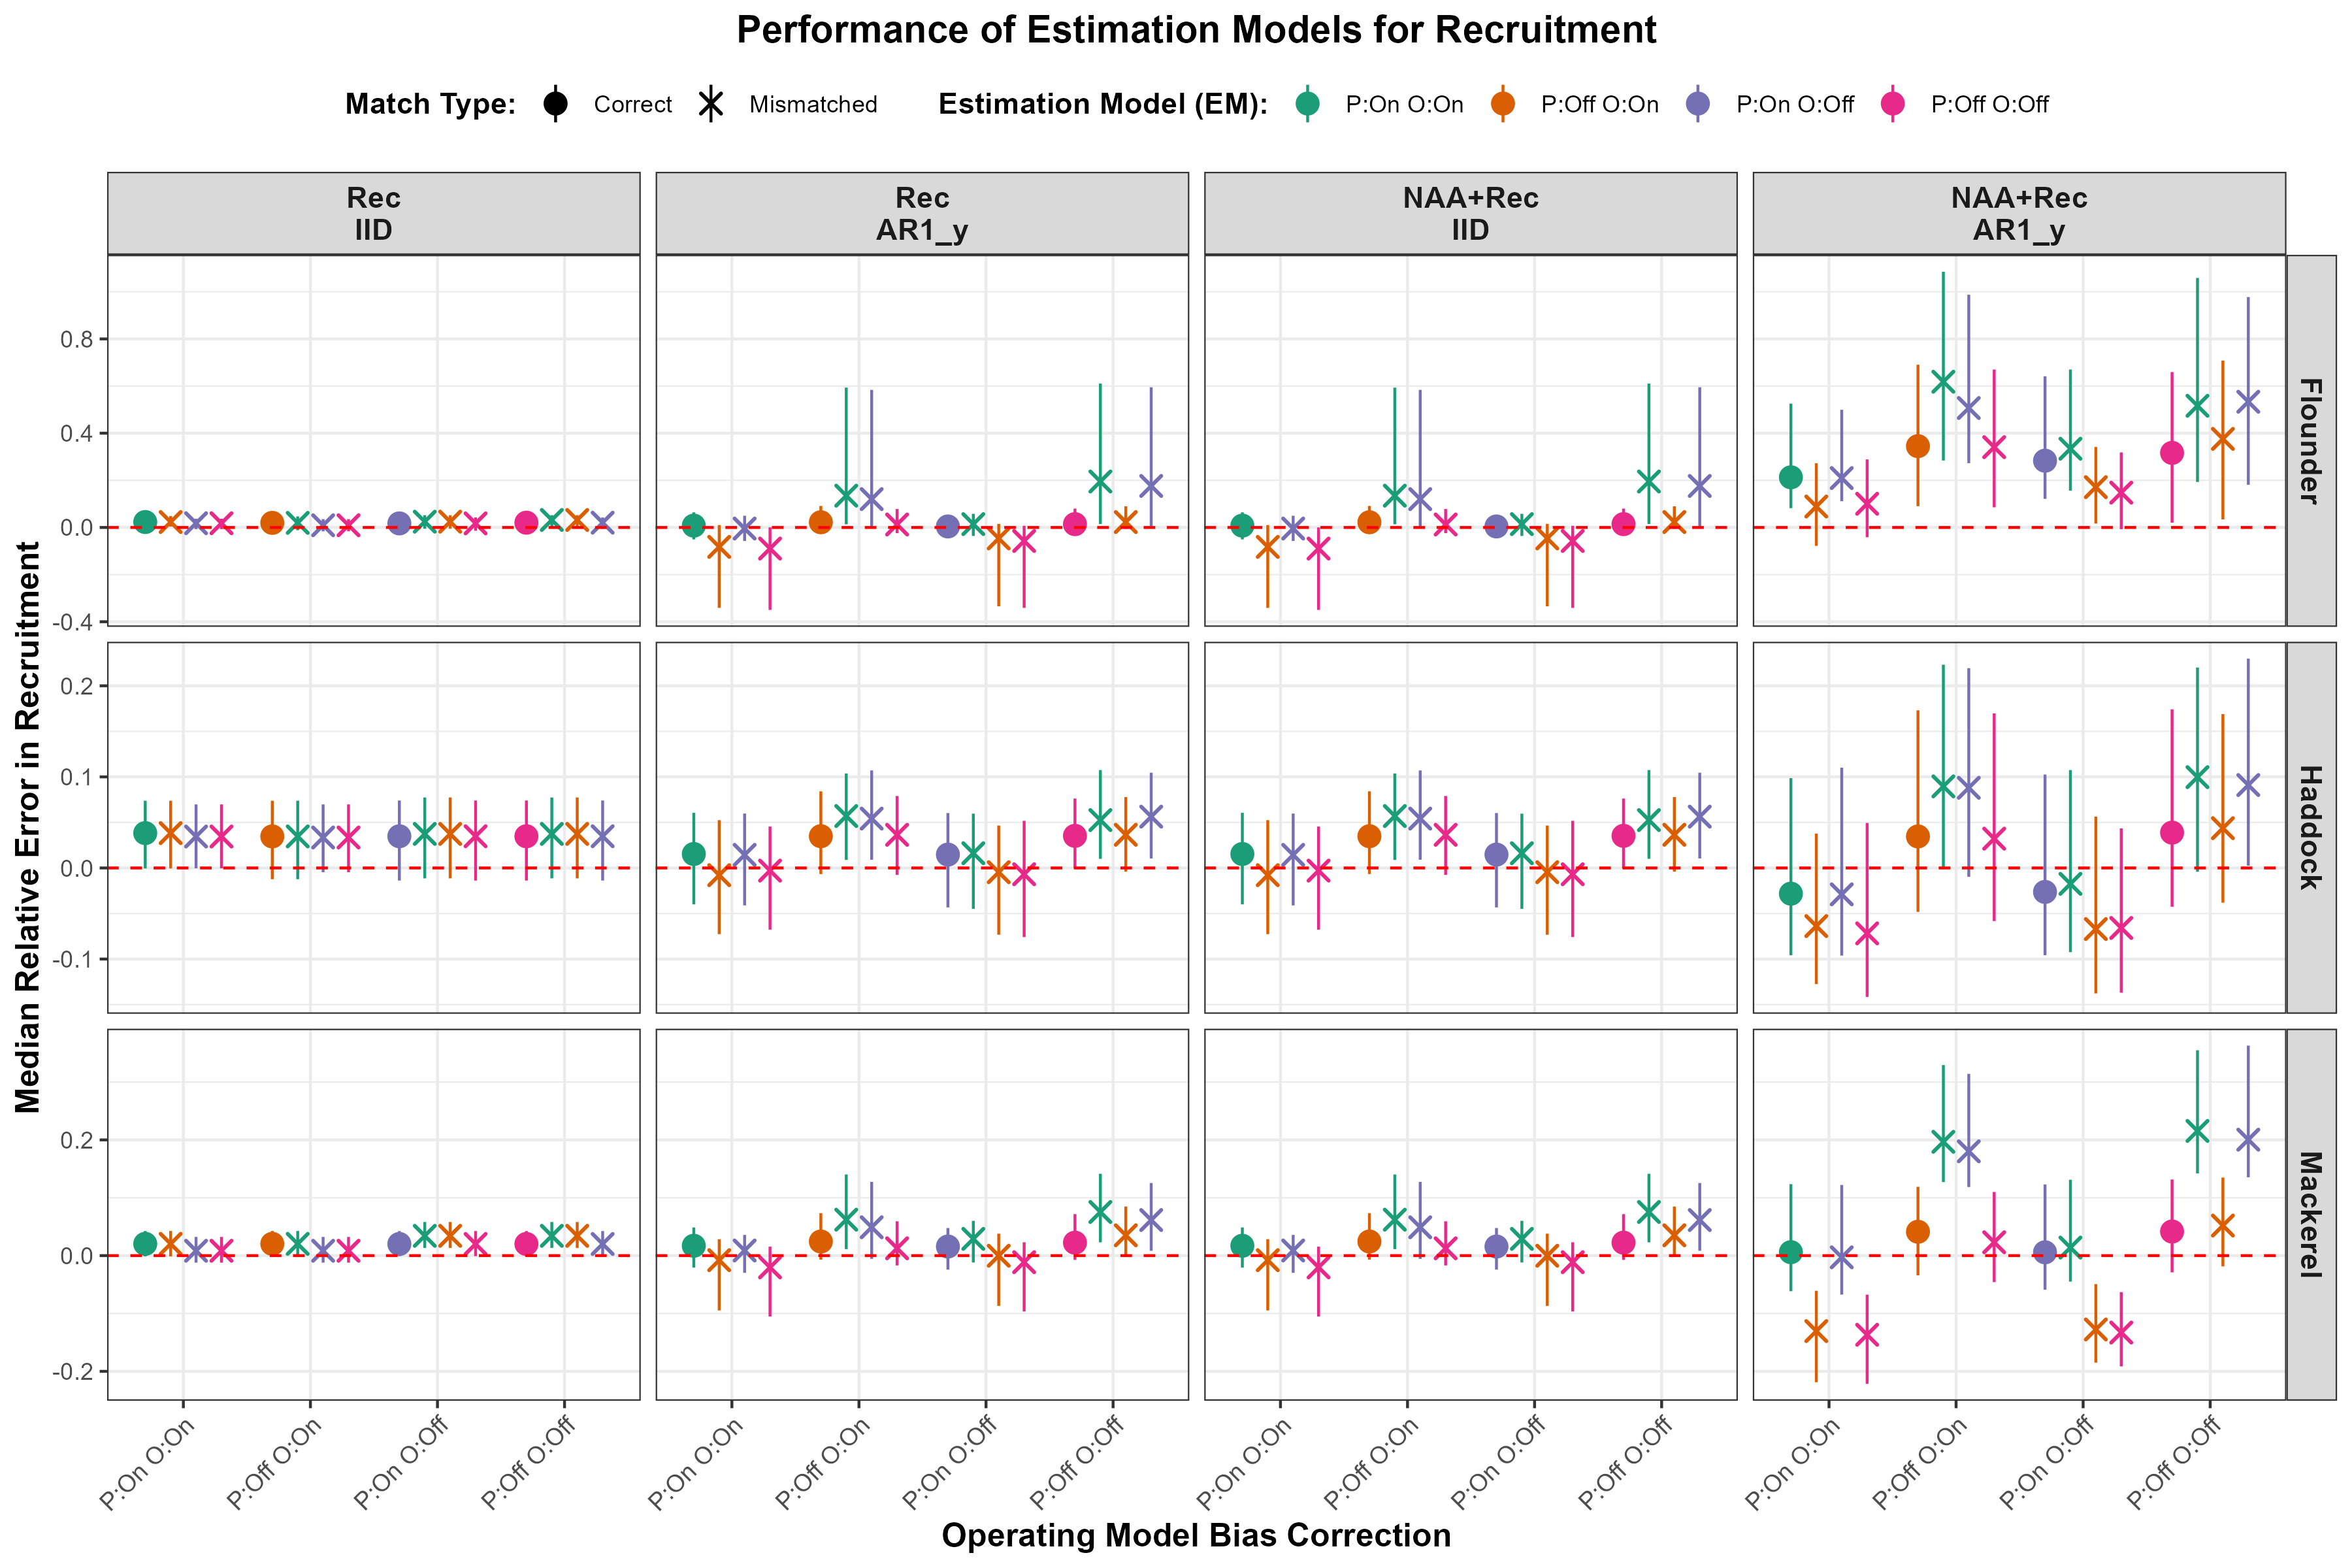
\includegraphics[width=\textwidth]{Revised_Figures&Tables/OM_EM_Comparison_Plot_Rec.PNG}
\caption{Median relative error of recruitment calculated for self-tests and cross-tests. ``Rec RE'' and ``Rec+NAA RE'' in the top facet indicate operating models (OMs) with only recruitment random effects and both recruitment and $NAA$ random effects, respectively.}
\label{fig:supp_OM_EM_Comparison_Plot_Rec}
\end{figure}

\begin{figure}[H]
\centering
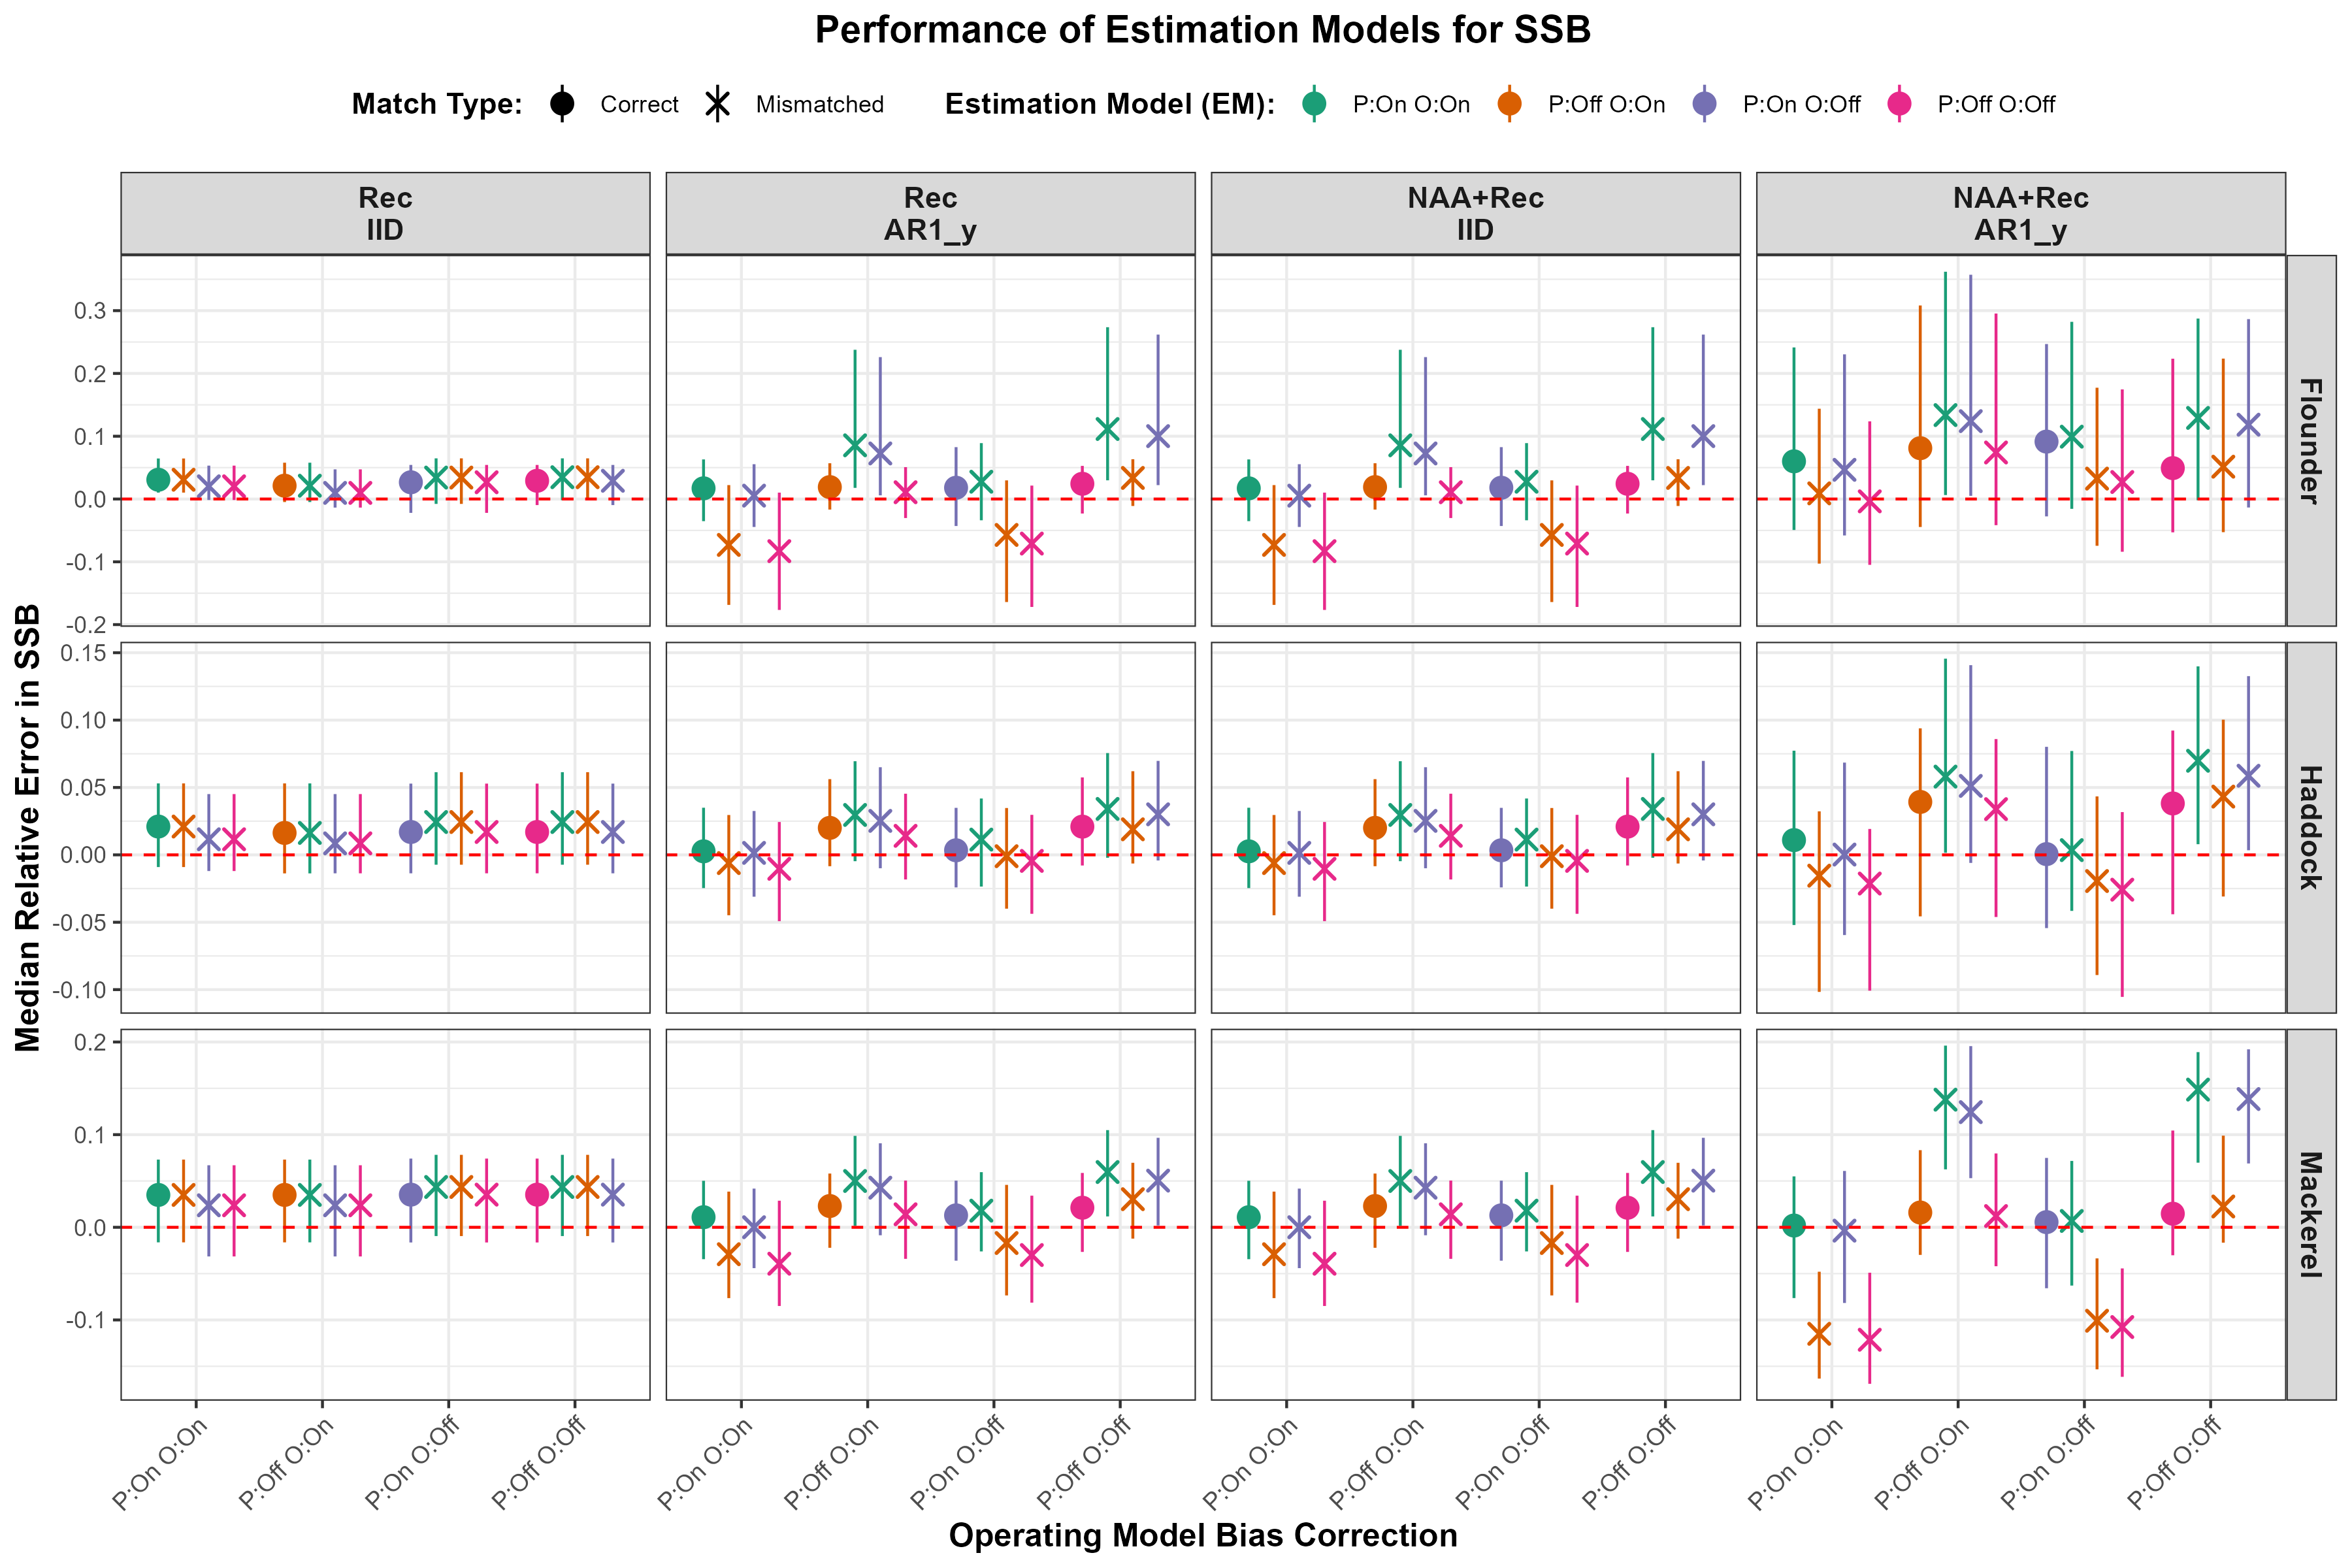
\includegraphics[width=\textwidth]{Revised_Figures&Tables/OM_EM_Comparison_Plot_SSB.PNG}
\caption{Median relative error of $SSB$ calculated for self-tests and cross-tests. ``Rec RE'' and ``Rec+NAA RE'' in the top facet indicate operating models (OMs) with only recruitment random effects and both recruitment and $NAA$ random effects, respectively.}
\label{fig:supp_OM_EM_Comparison_Plot_SSB}
\end{figure}

\begin{figure}[H]
    \centering
    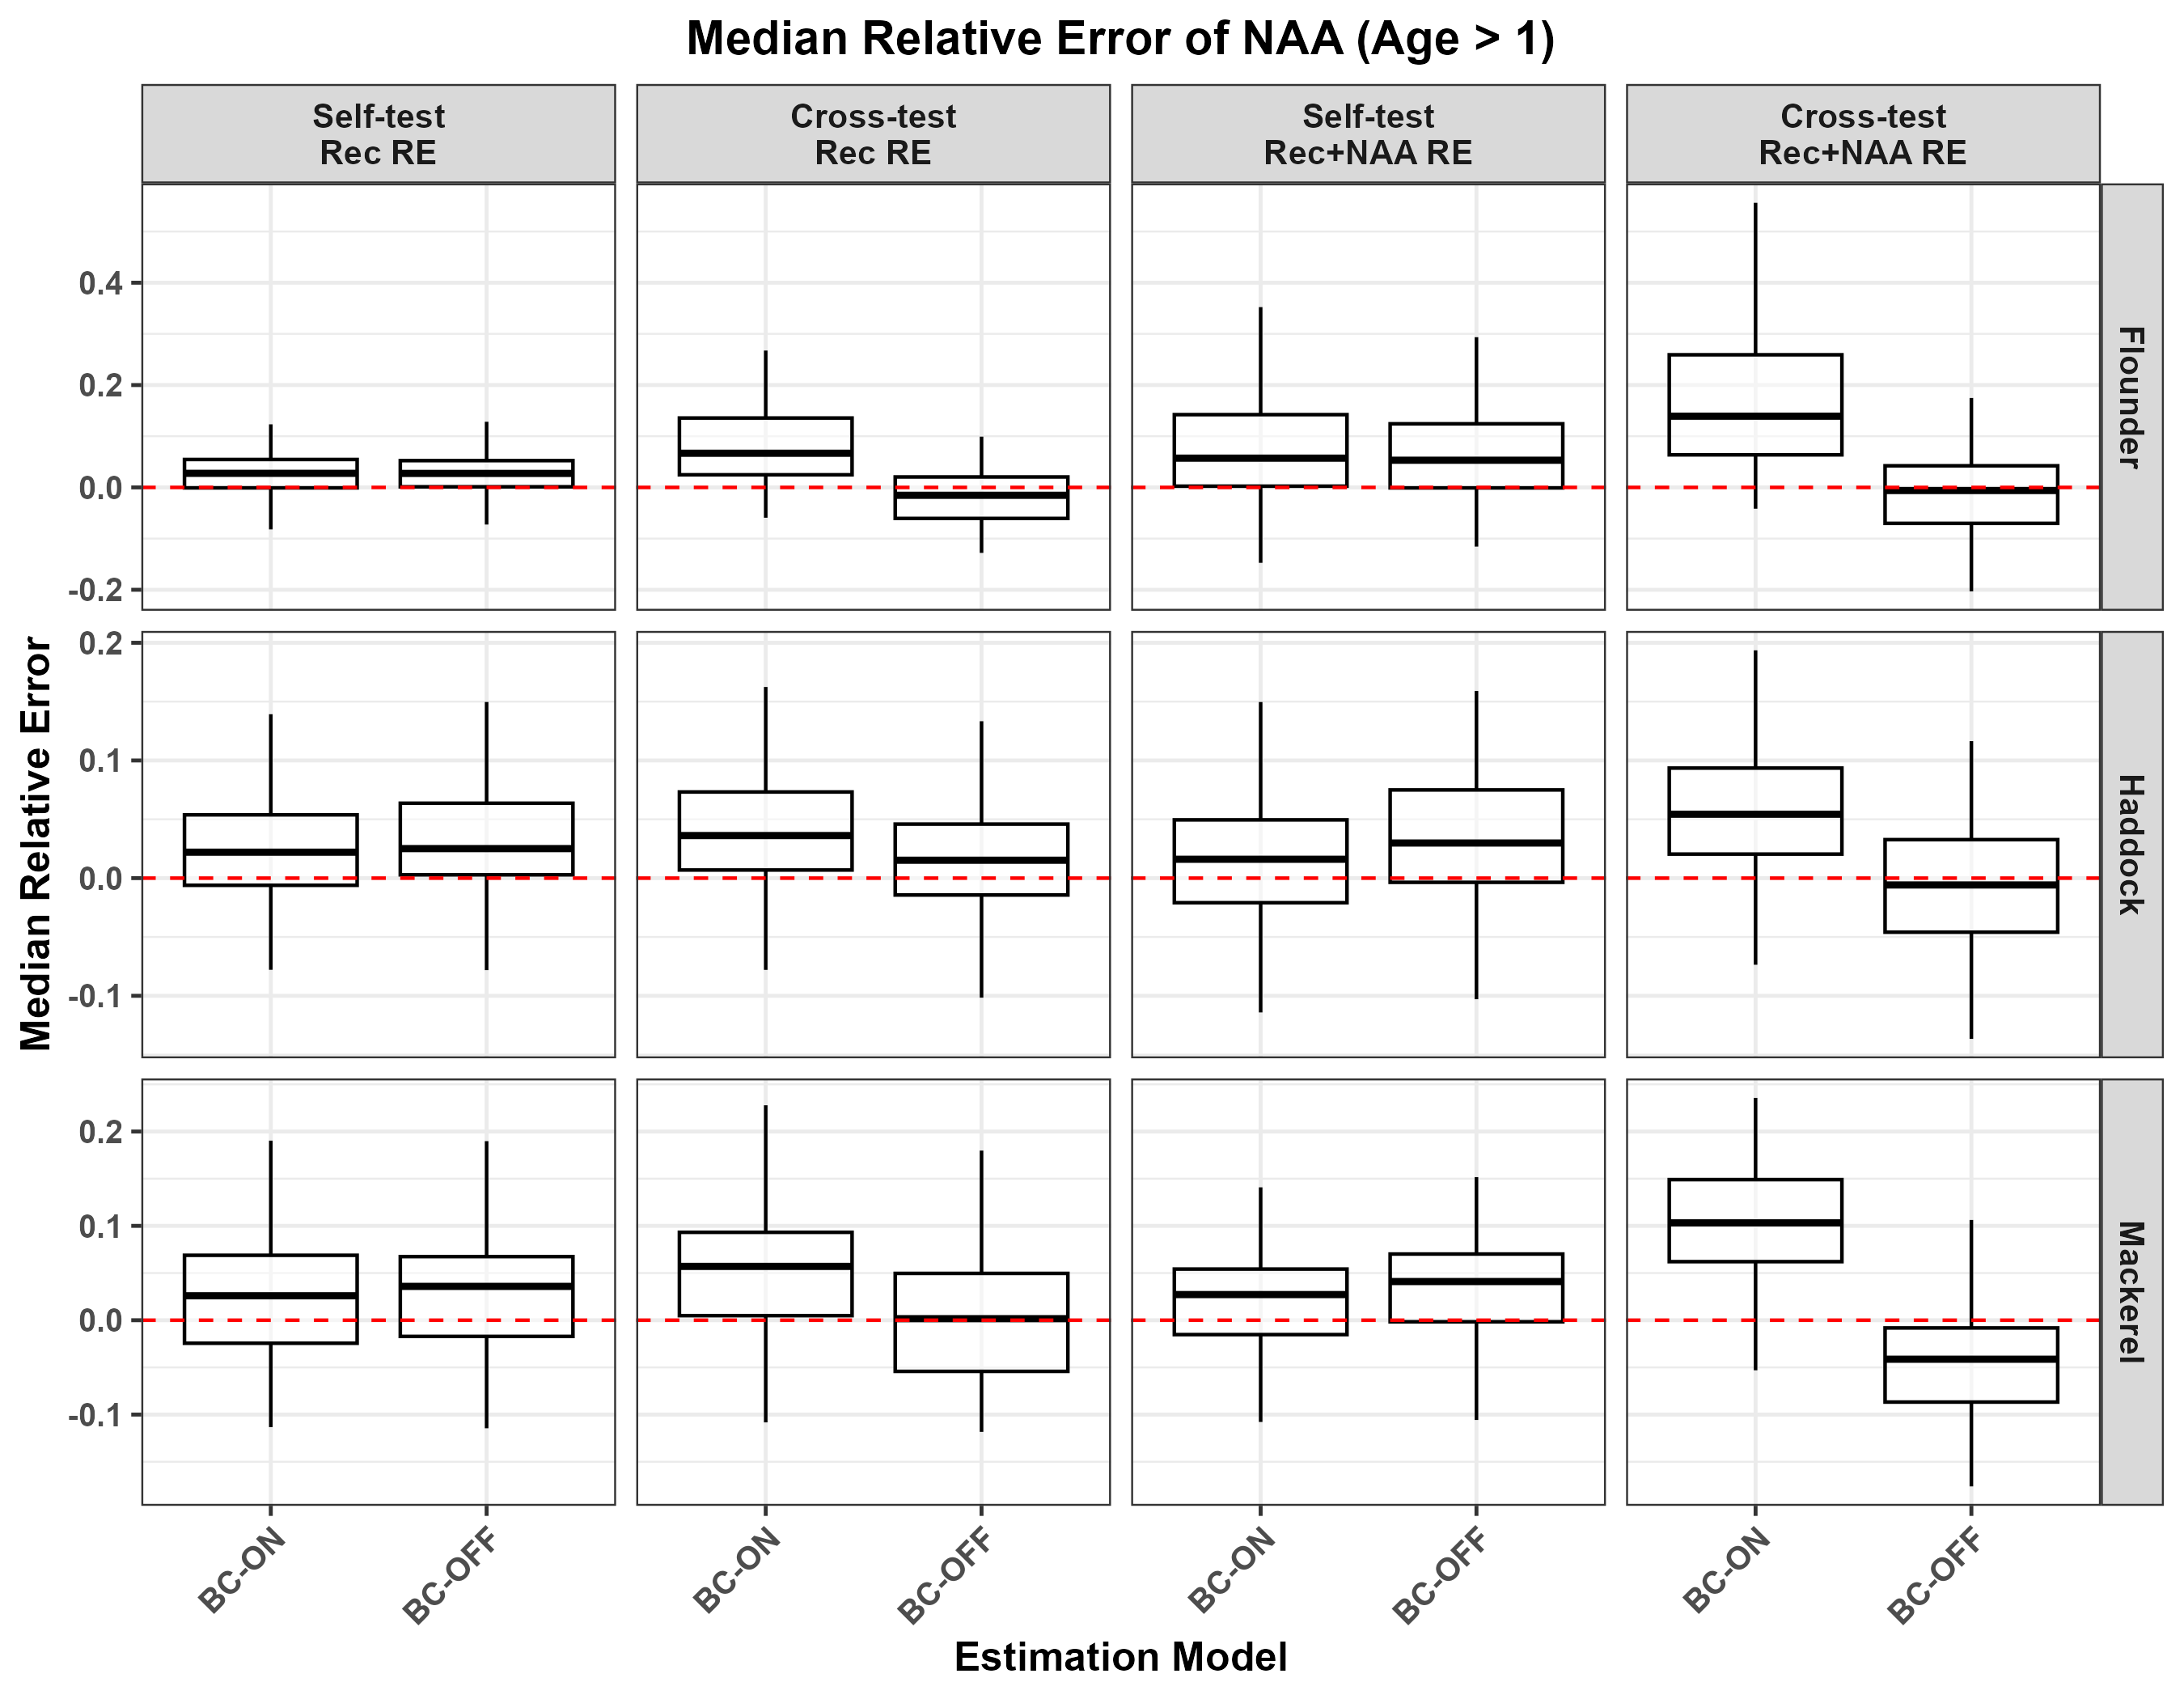
\includegraphics[width=\textwidth]{Revised_Figures&Tables/Median_NAA.PNG}
    \caption{Median relative error of $NAA$ calculated for self-tests and cross-tests. ``Rec RE'' and ``Rec+NAA RE'' in the top facet indicate operating models (OMs) with only recruitment random effects and both recruitment and $NAA$ random effects, respectively.}
    \label{fig:supp_Median_NAA}
\end{figure}

\begin{figure}[H]
    \centering
    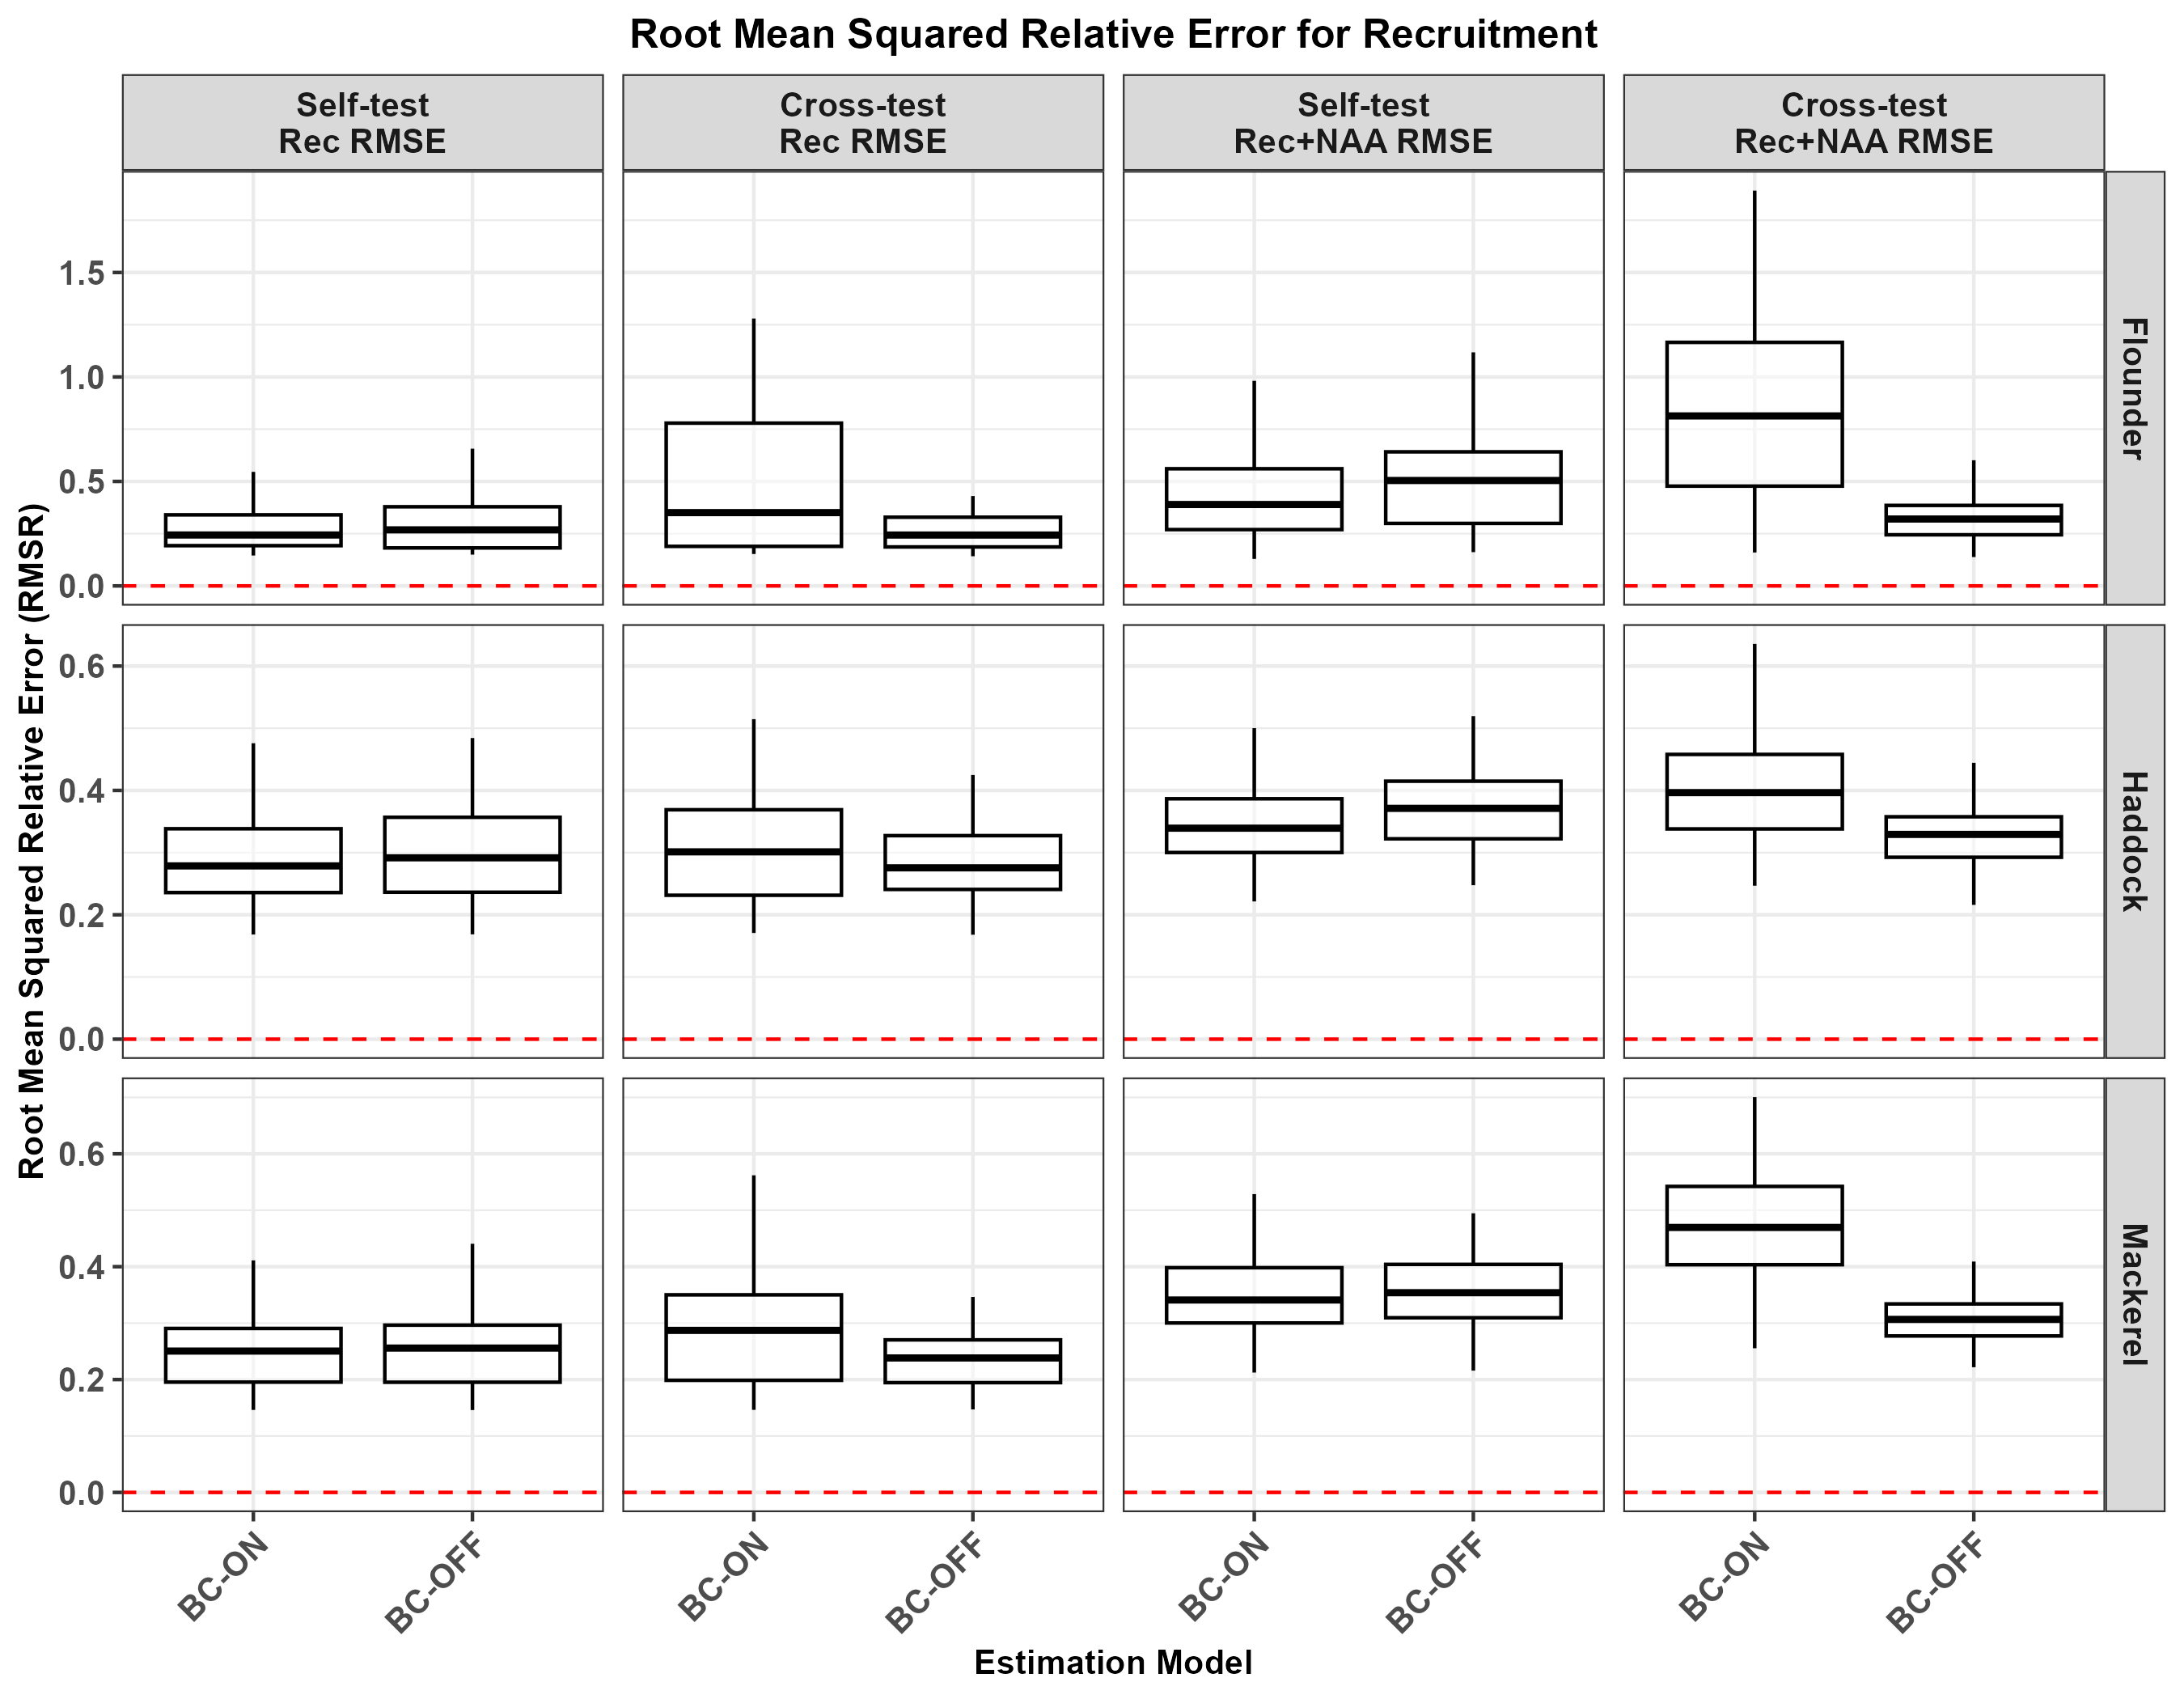
\includegraphics[width=\textwidth]{Revised_Figures&Tables/RMSR_Rec.PNG}
    \caption{Root mean squared relative error (RMSR) of recruitment calculated for self-tests and cross-tests. ``Rec RE'' and ``Rec+NAA RE'' in the top facet indicate operating models (OMs) with only recruitment random effects and both recruitment and $NAA$ random effects, respectively.}
    \label{fig:supp_Rec_RMSR}
\end{figure}

\begin{figure}[H]
    \centering
    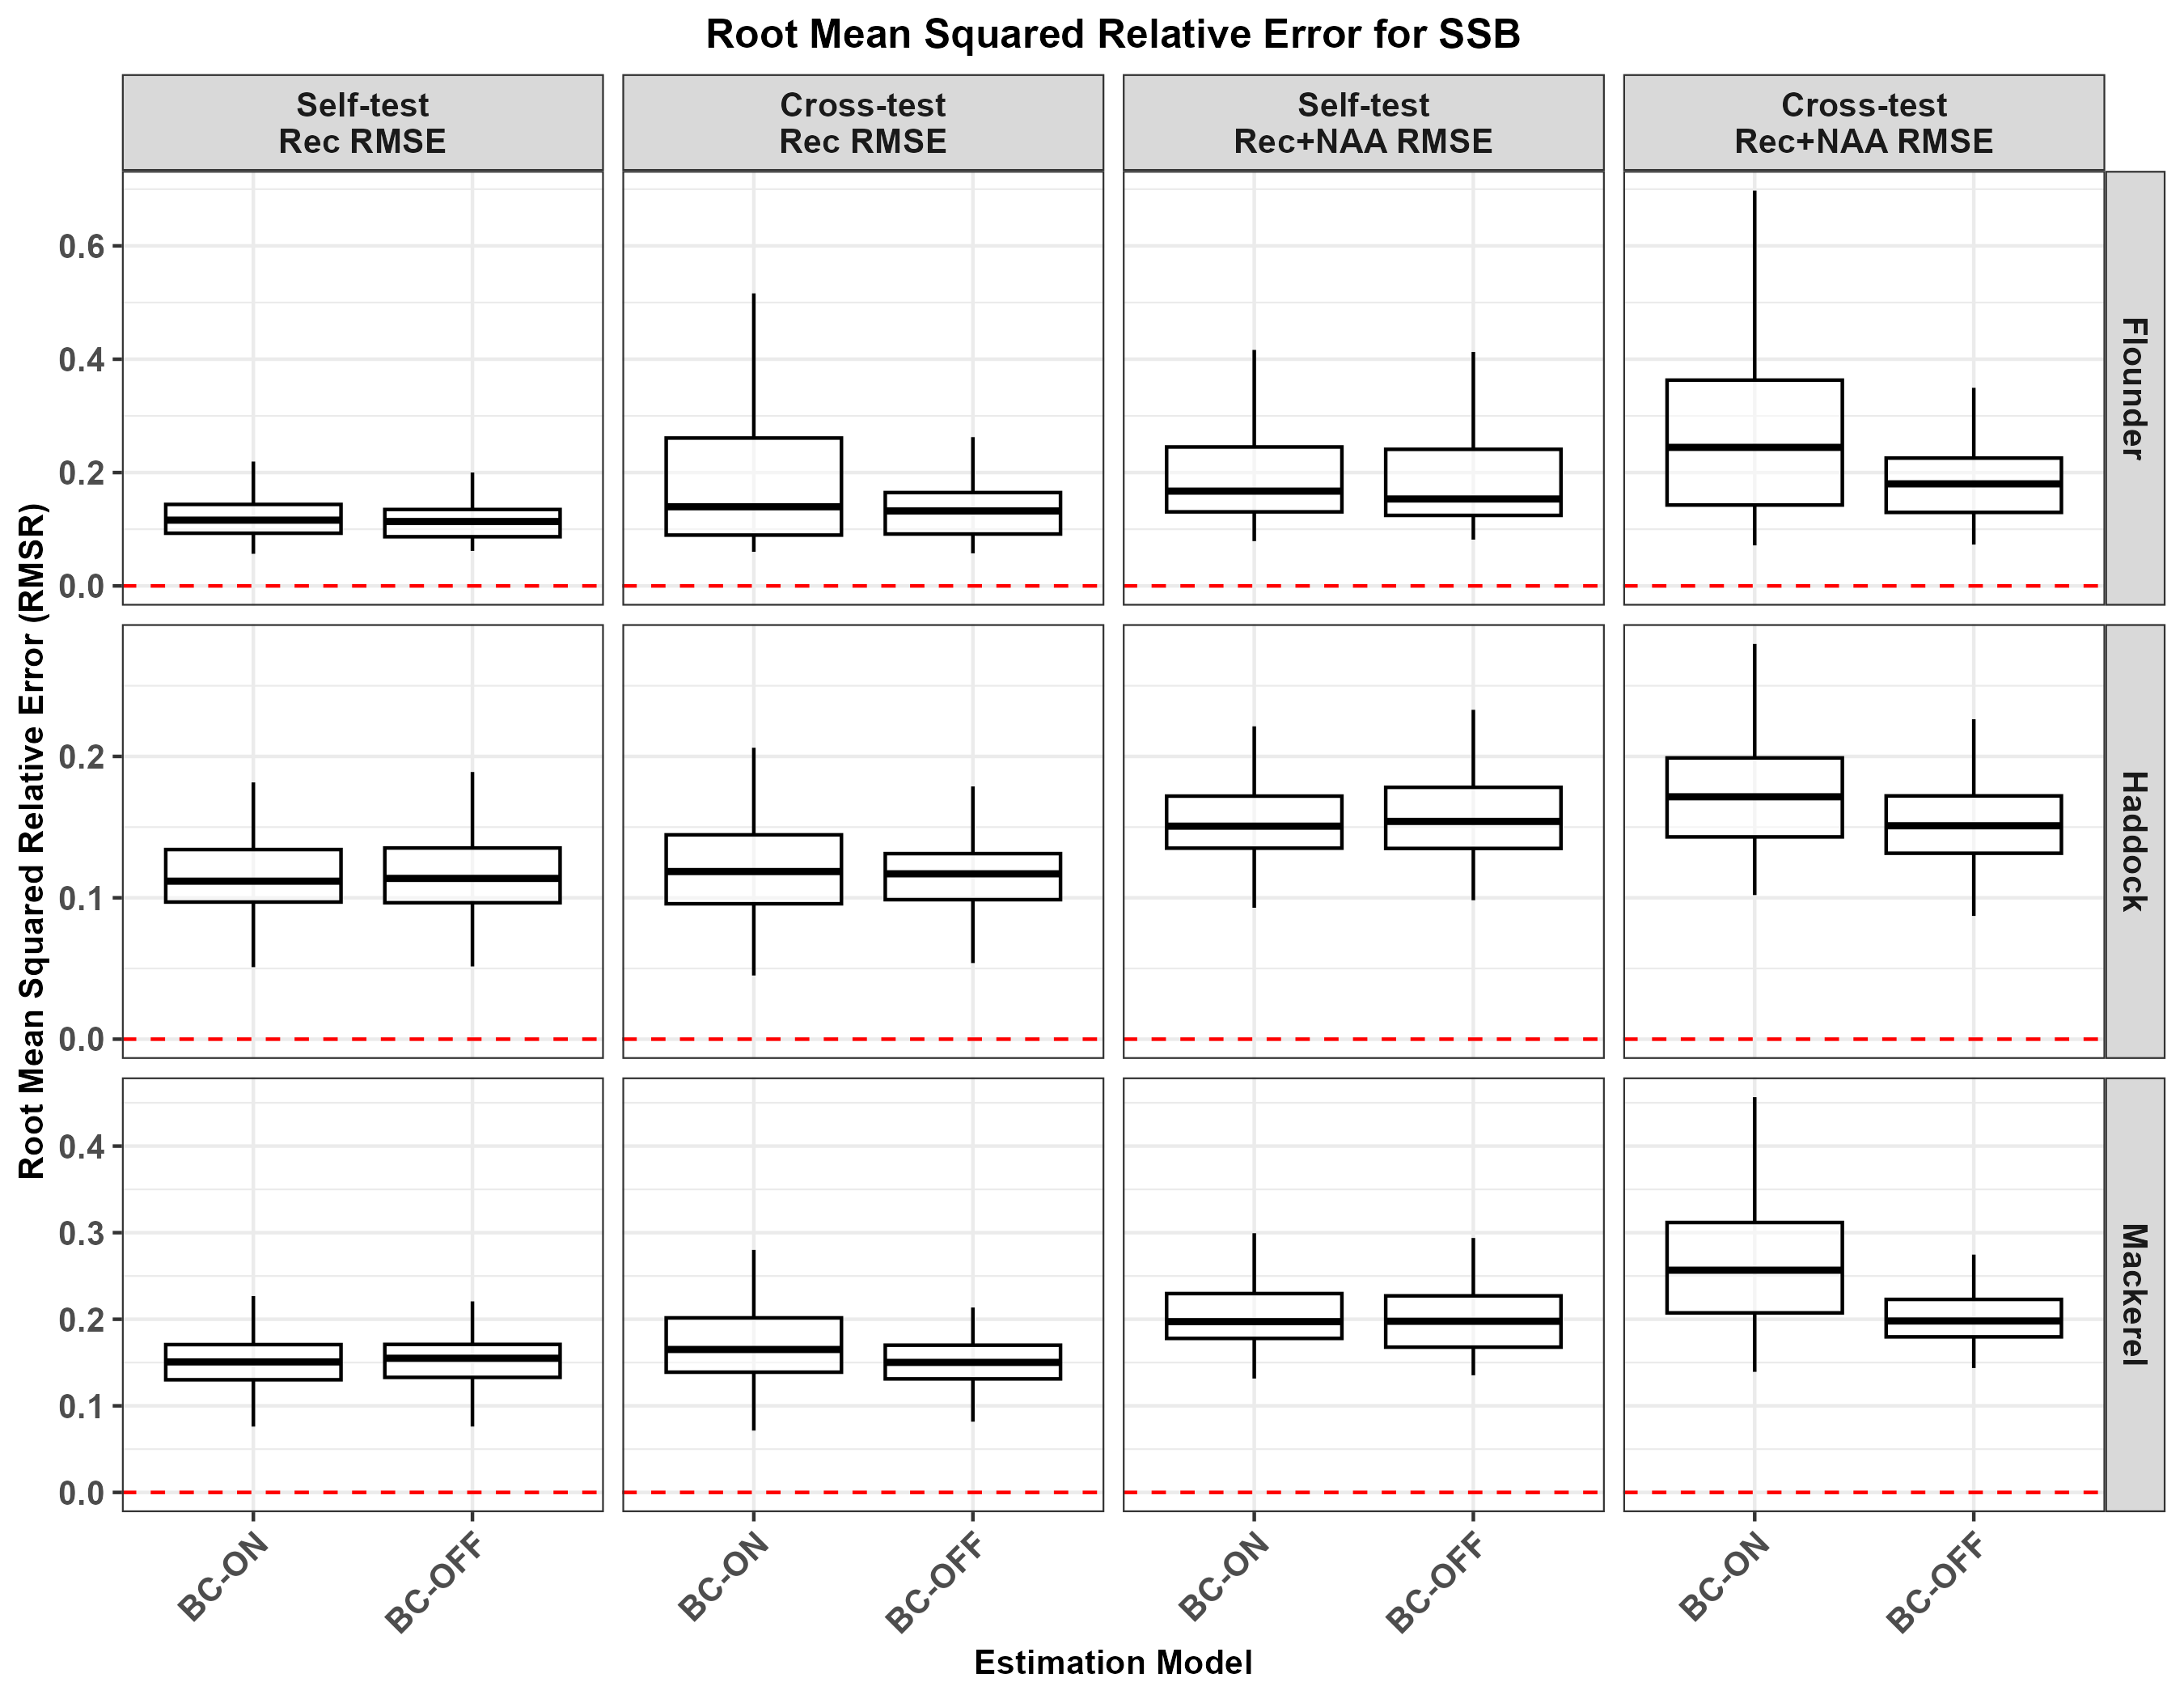
\includegraphics[width=\textwidth]{Revised_Figures&Tables/RMSR_SSB.PNG}
    \caption{Root mean squared relative error (RMSR) of $SSB$ calculated for self-tests and cross-tests. ``Rec RE'' and ``Rec+NAA RE'' in the top facet indicate operating models (OMs) with only recruitment random effects and both recruitment and $NAA$ random effects, respectively.}
    \label{fig:supp_SSB_RMSR}
\end{figure}

\begin{figure}[H]
    \centering
    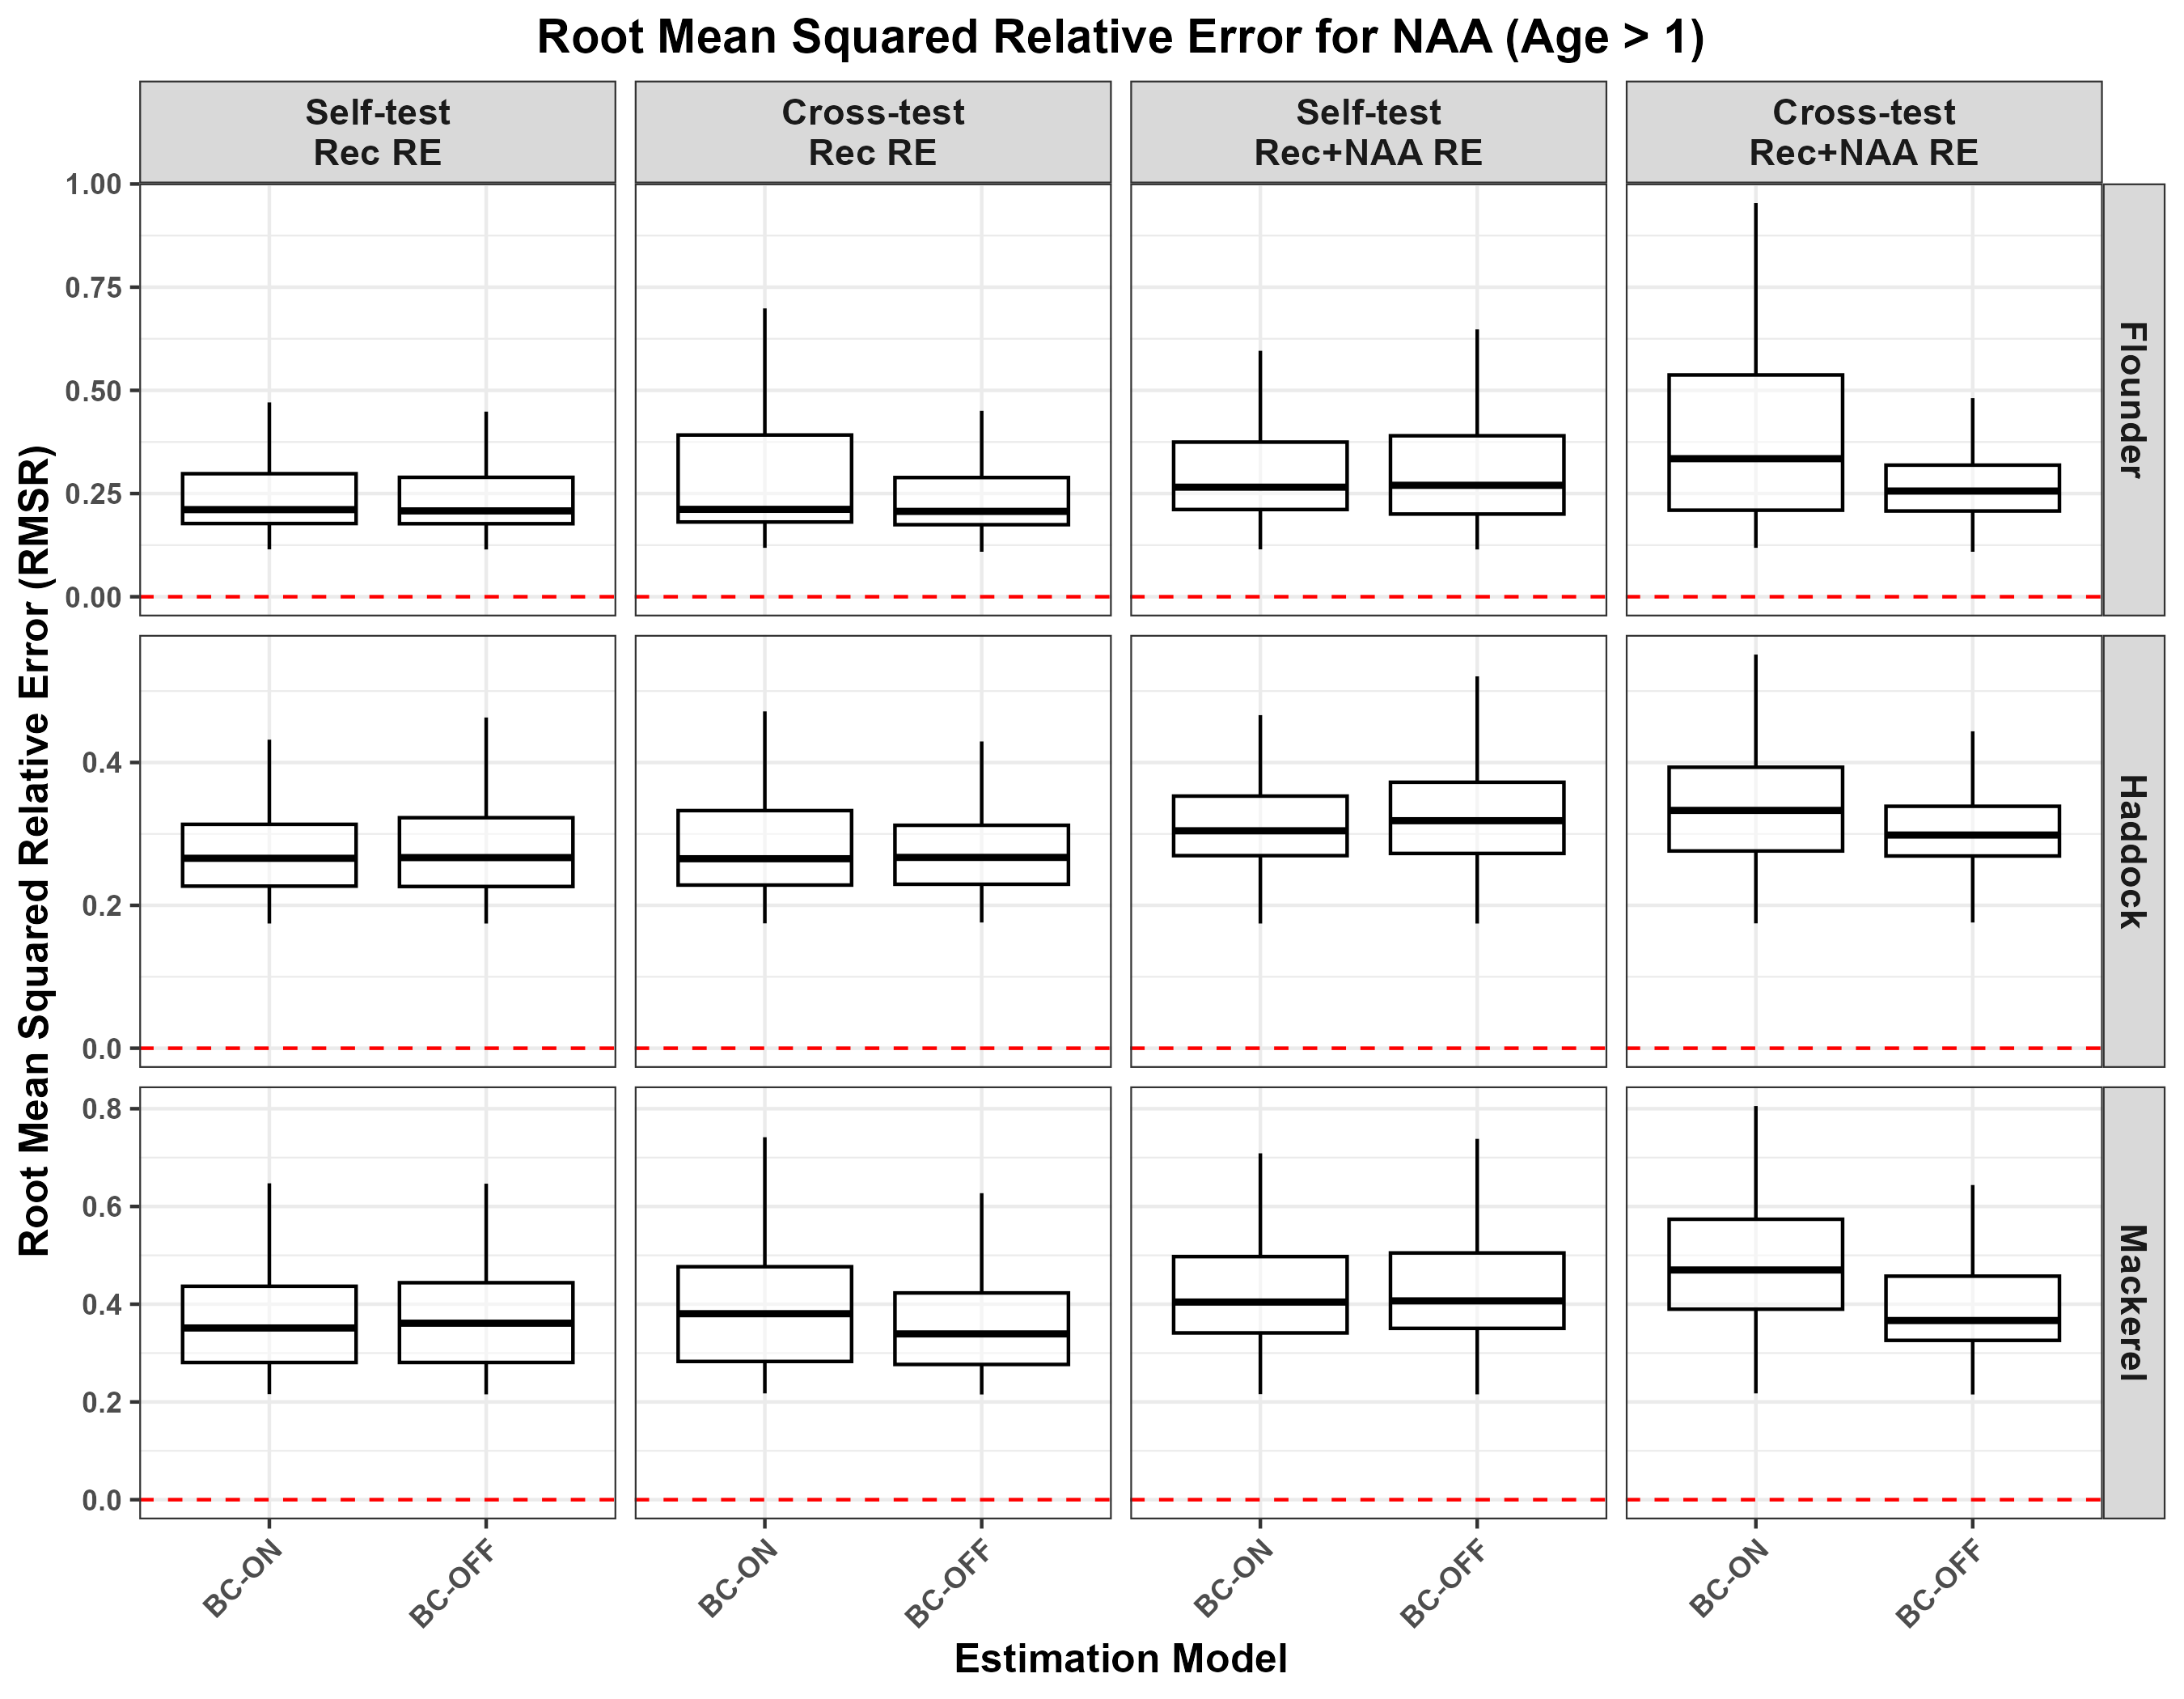
\includegraphics[width=\textwidth]{Revised_Figures&Tables/RMSR_NAA.PNG}
    \caption{Root mean squared relative error (RMSR) of $NAA$ calculated for self-tests and cross-tests. ``Rec RE'' and ``Rec+NAA RE'' in the top facet indicate operating models (OMs) with only recruitment random effects and both recruitment and $NAA$ random effects, respectively.}
    \label{fig:supp_NAA_RMSR}
\end{figure}

\begin{figure}[H]
    \centering
    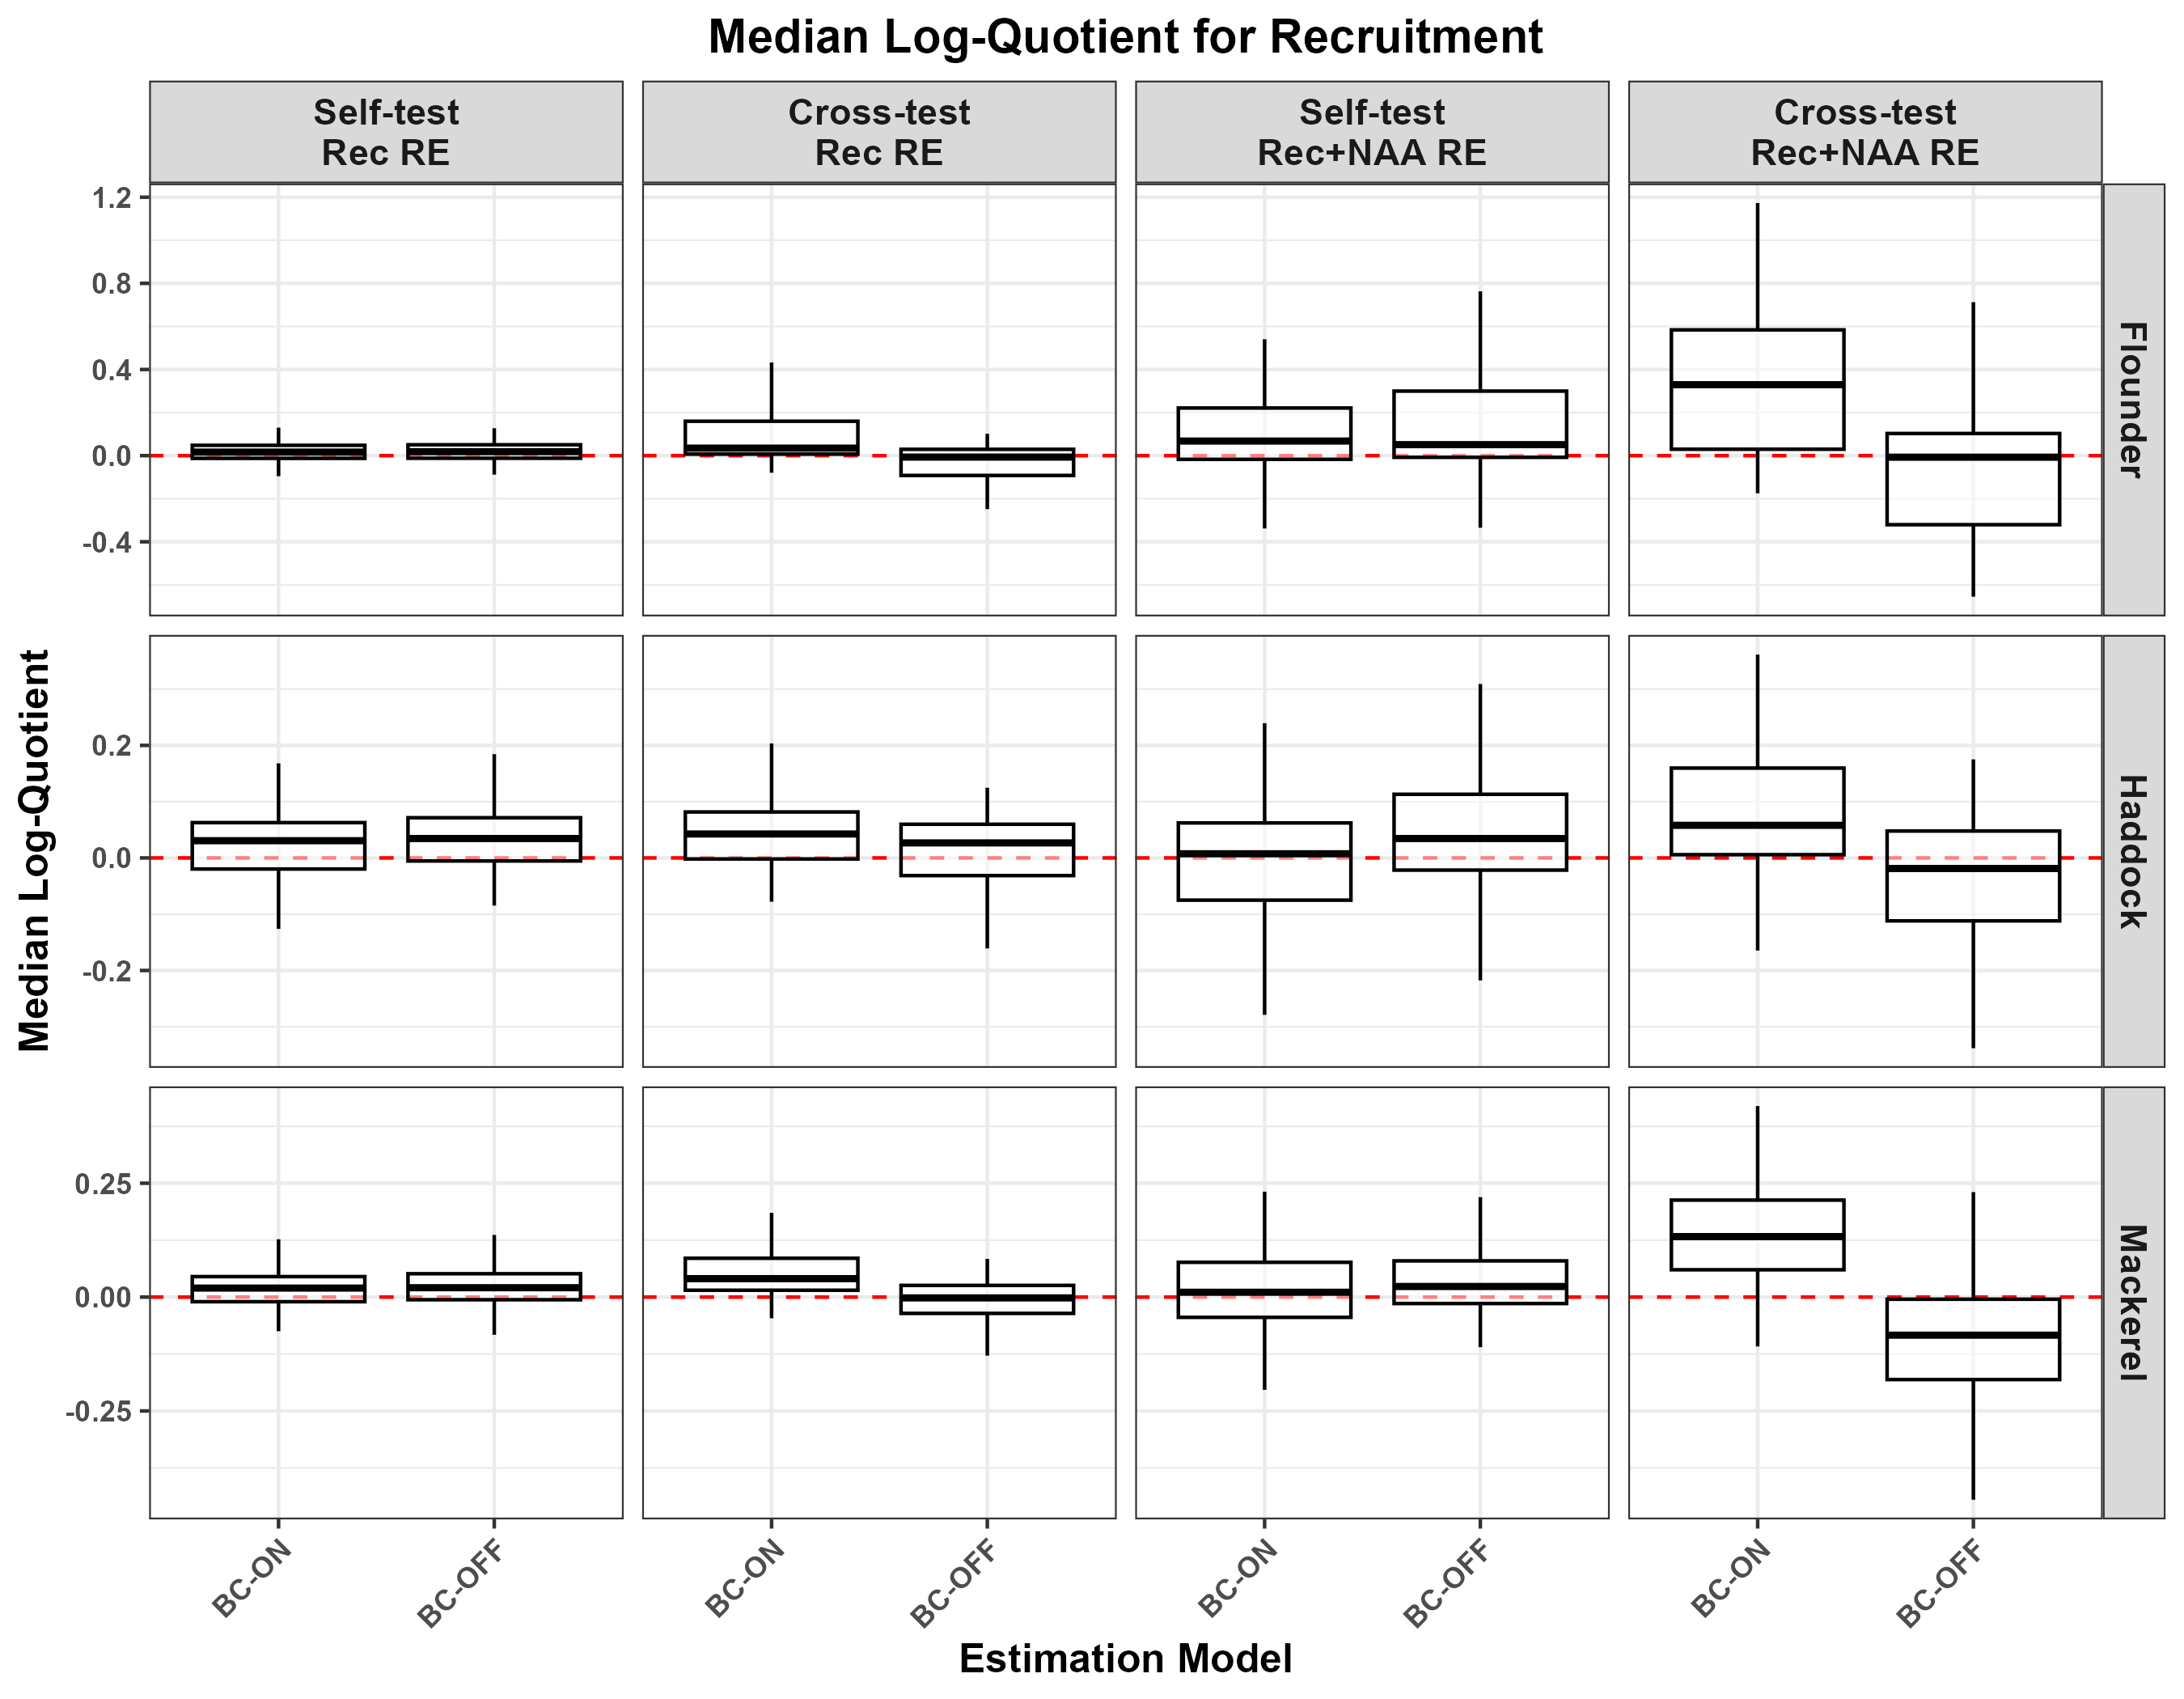
\includegraphics[width=\textwidth]{Revised_Figures&Tables/MdLQ_Rec.PNG}
    \caption{Median log-quotient (MdLQ) of recruitment calculated for self-tests and cross-tests. ``Rec RE'' and ``Rec+NAA RE'' in the top facet indicate operating models (OMs) with only recruitment random effects and both recruitment and $NAA$ random effects, respectively.}
    \label{fig:supp_Rec_MdLQ}
\end{figure}

\begin{figure}[H]
    \centering
    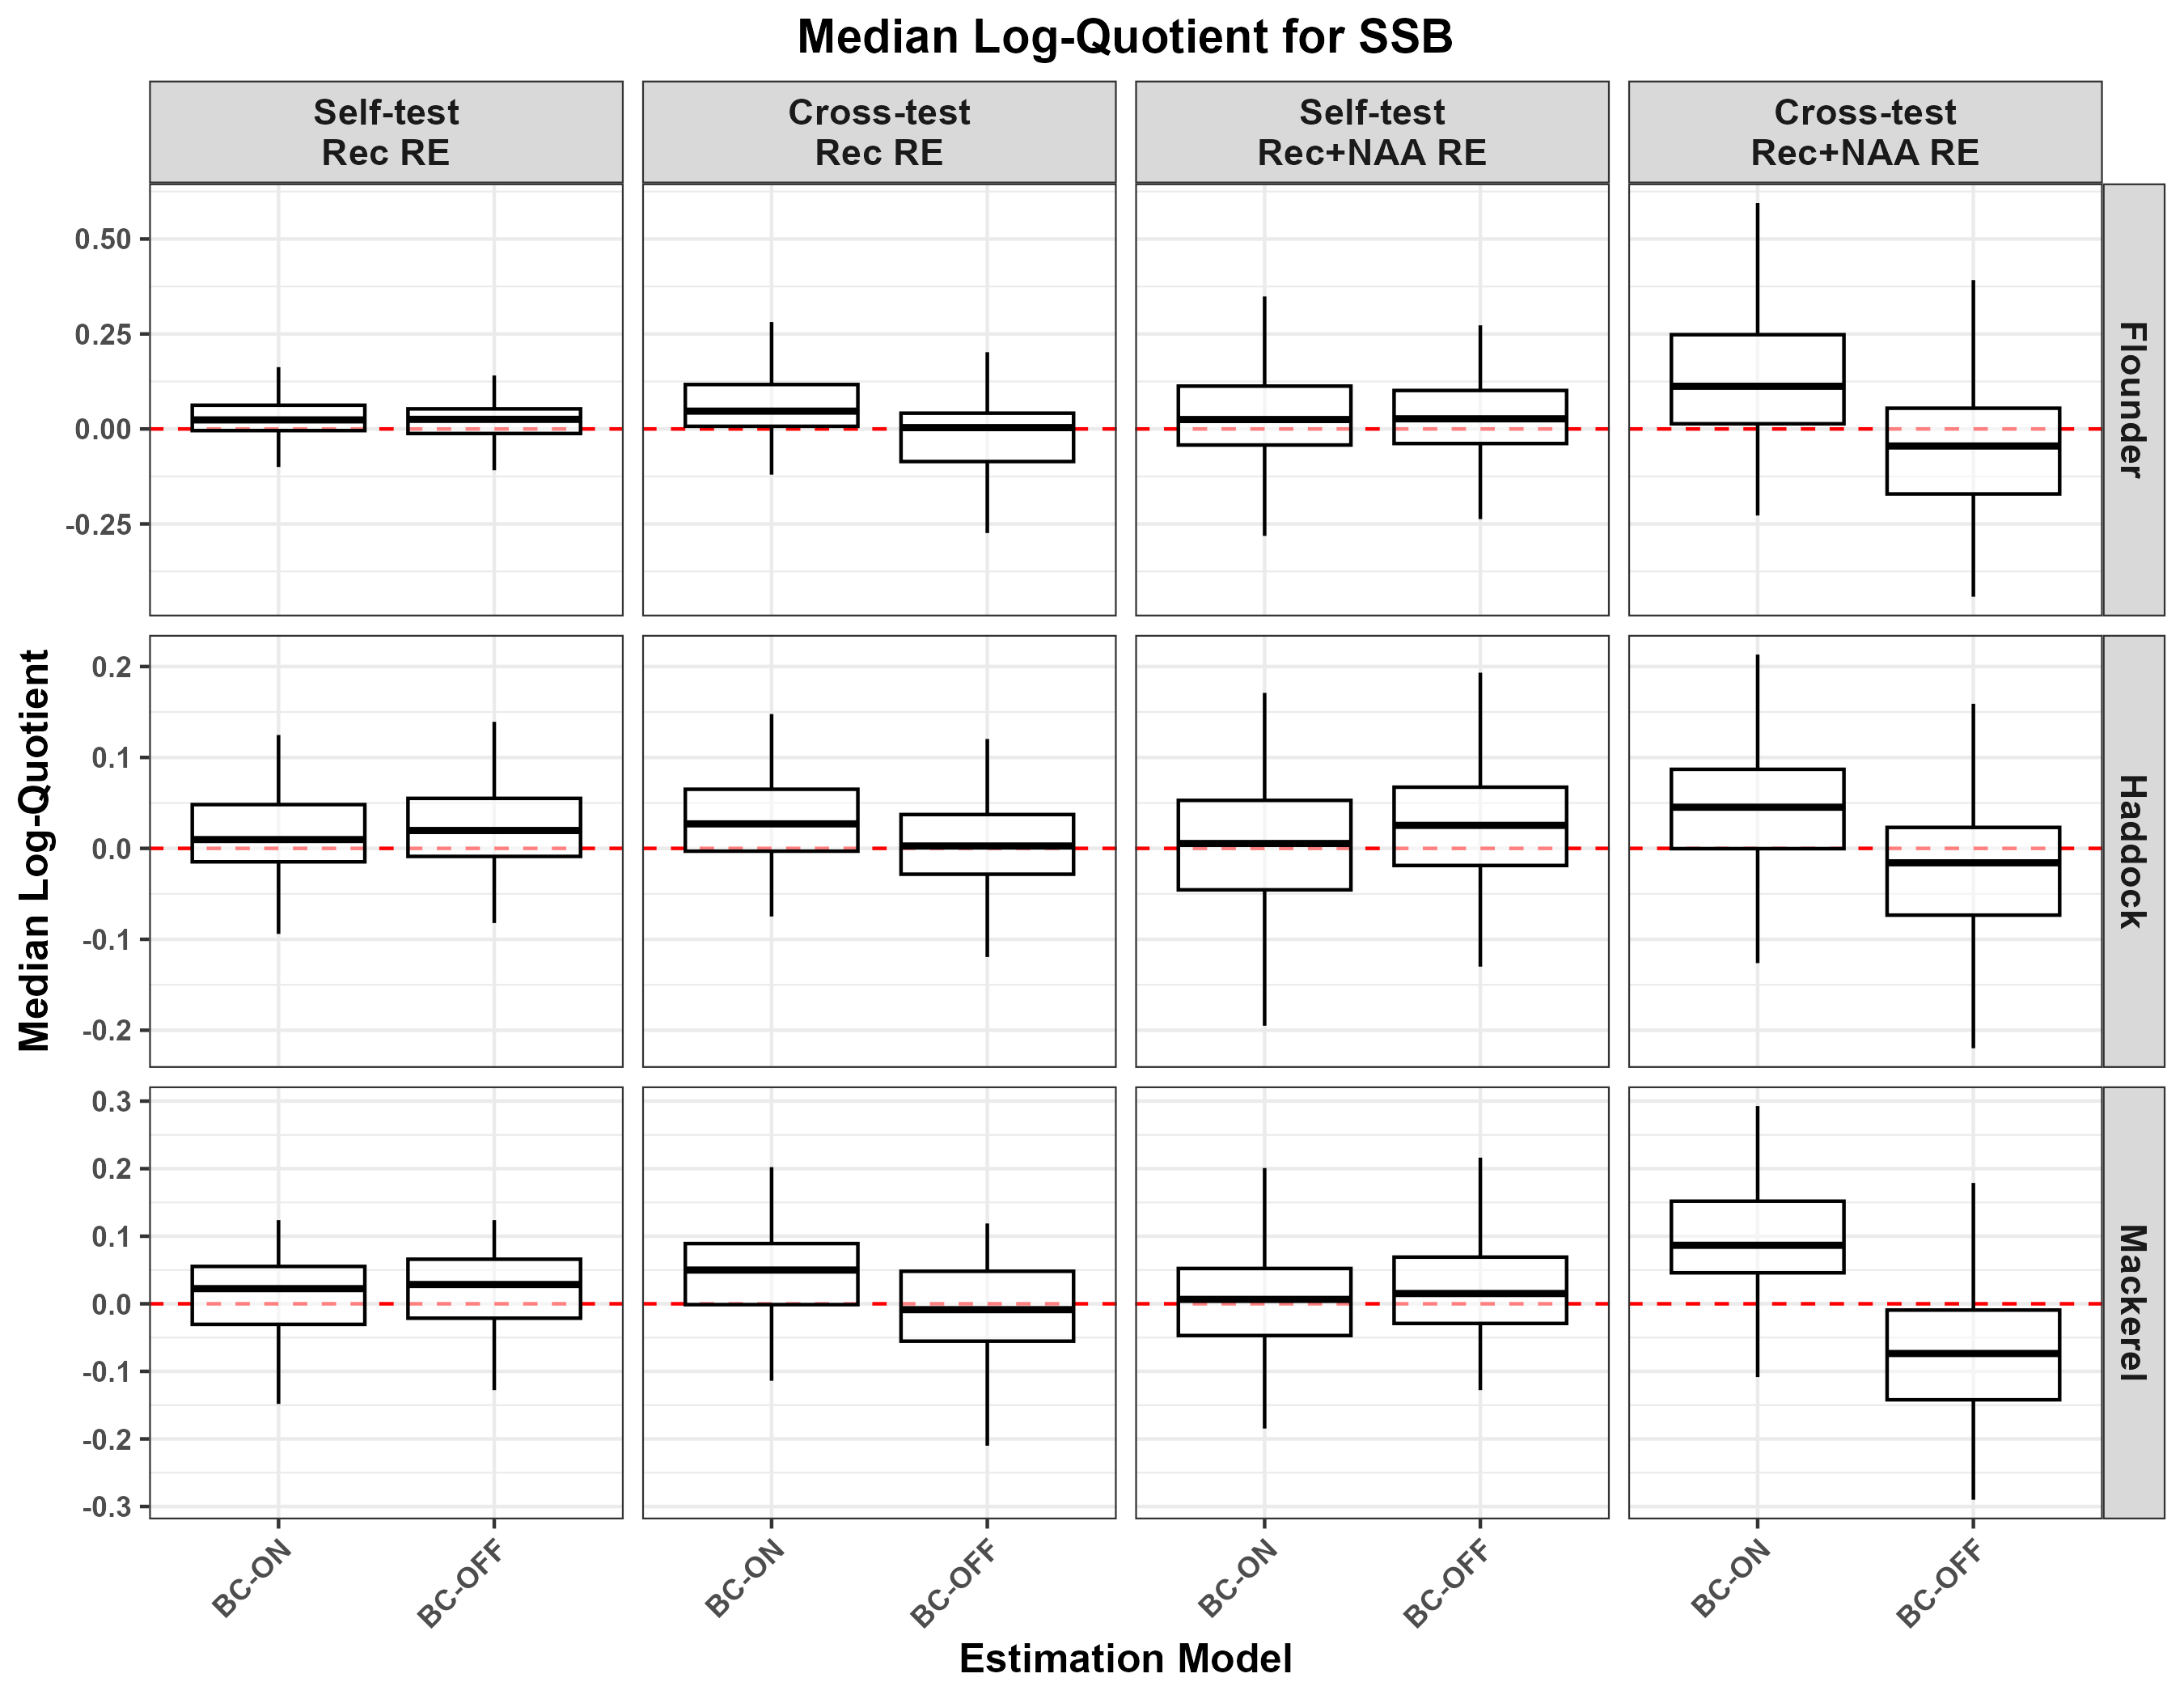
\includegraphics[width=\textwidth]{Revised_Figures&Tables/MdLQ_SSB.PNG}
    \caption{Median log-quotient (MdLQ) of $SSB$ calculated for self-tests and cross-tests. ``Rec RE'' and ``Rec+NAA RE'' in the top facet indicate operating models (OMs) with only recruitment random effects and both recruitment and $NAA$ random effects, respectively.}
    \label{fig:supp_SSB_MdLQ}
\end{figure}

\begin{figure}[H]
    \centering
    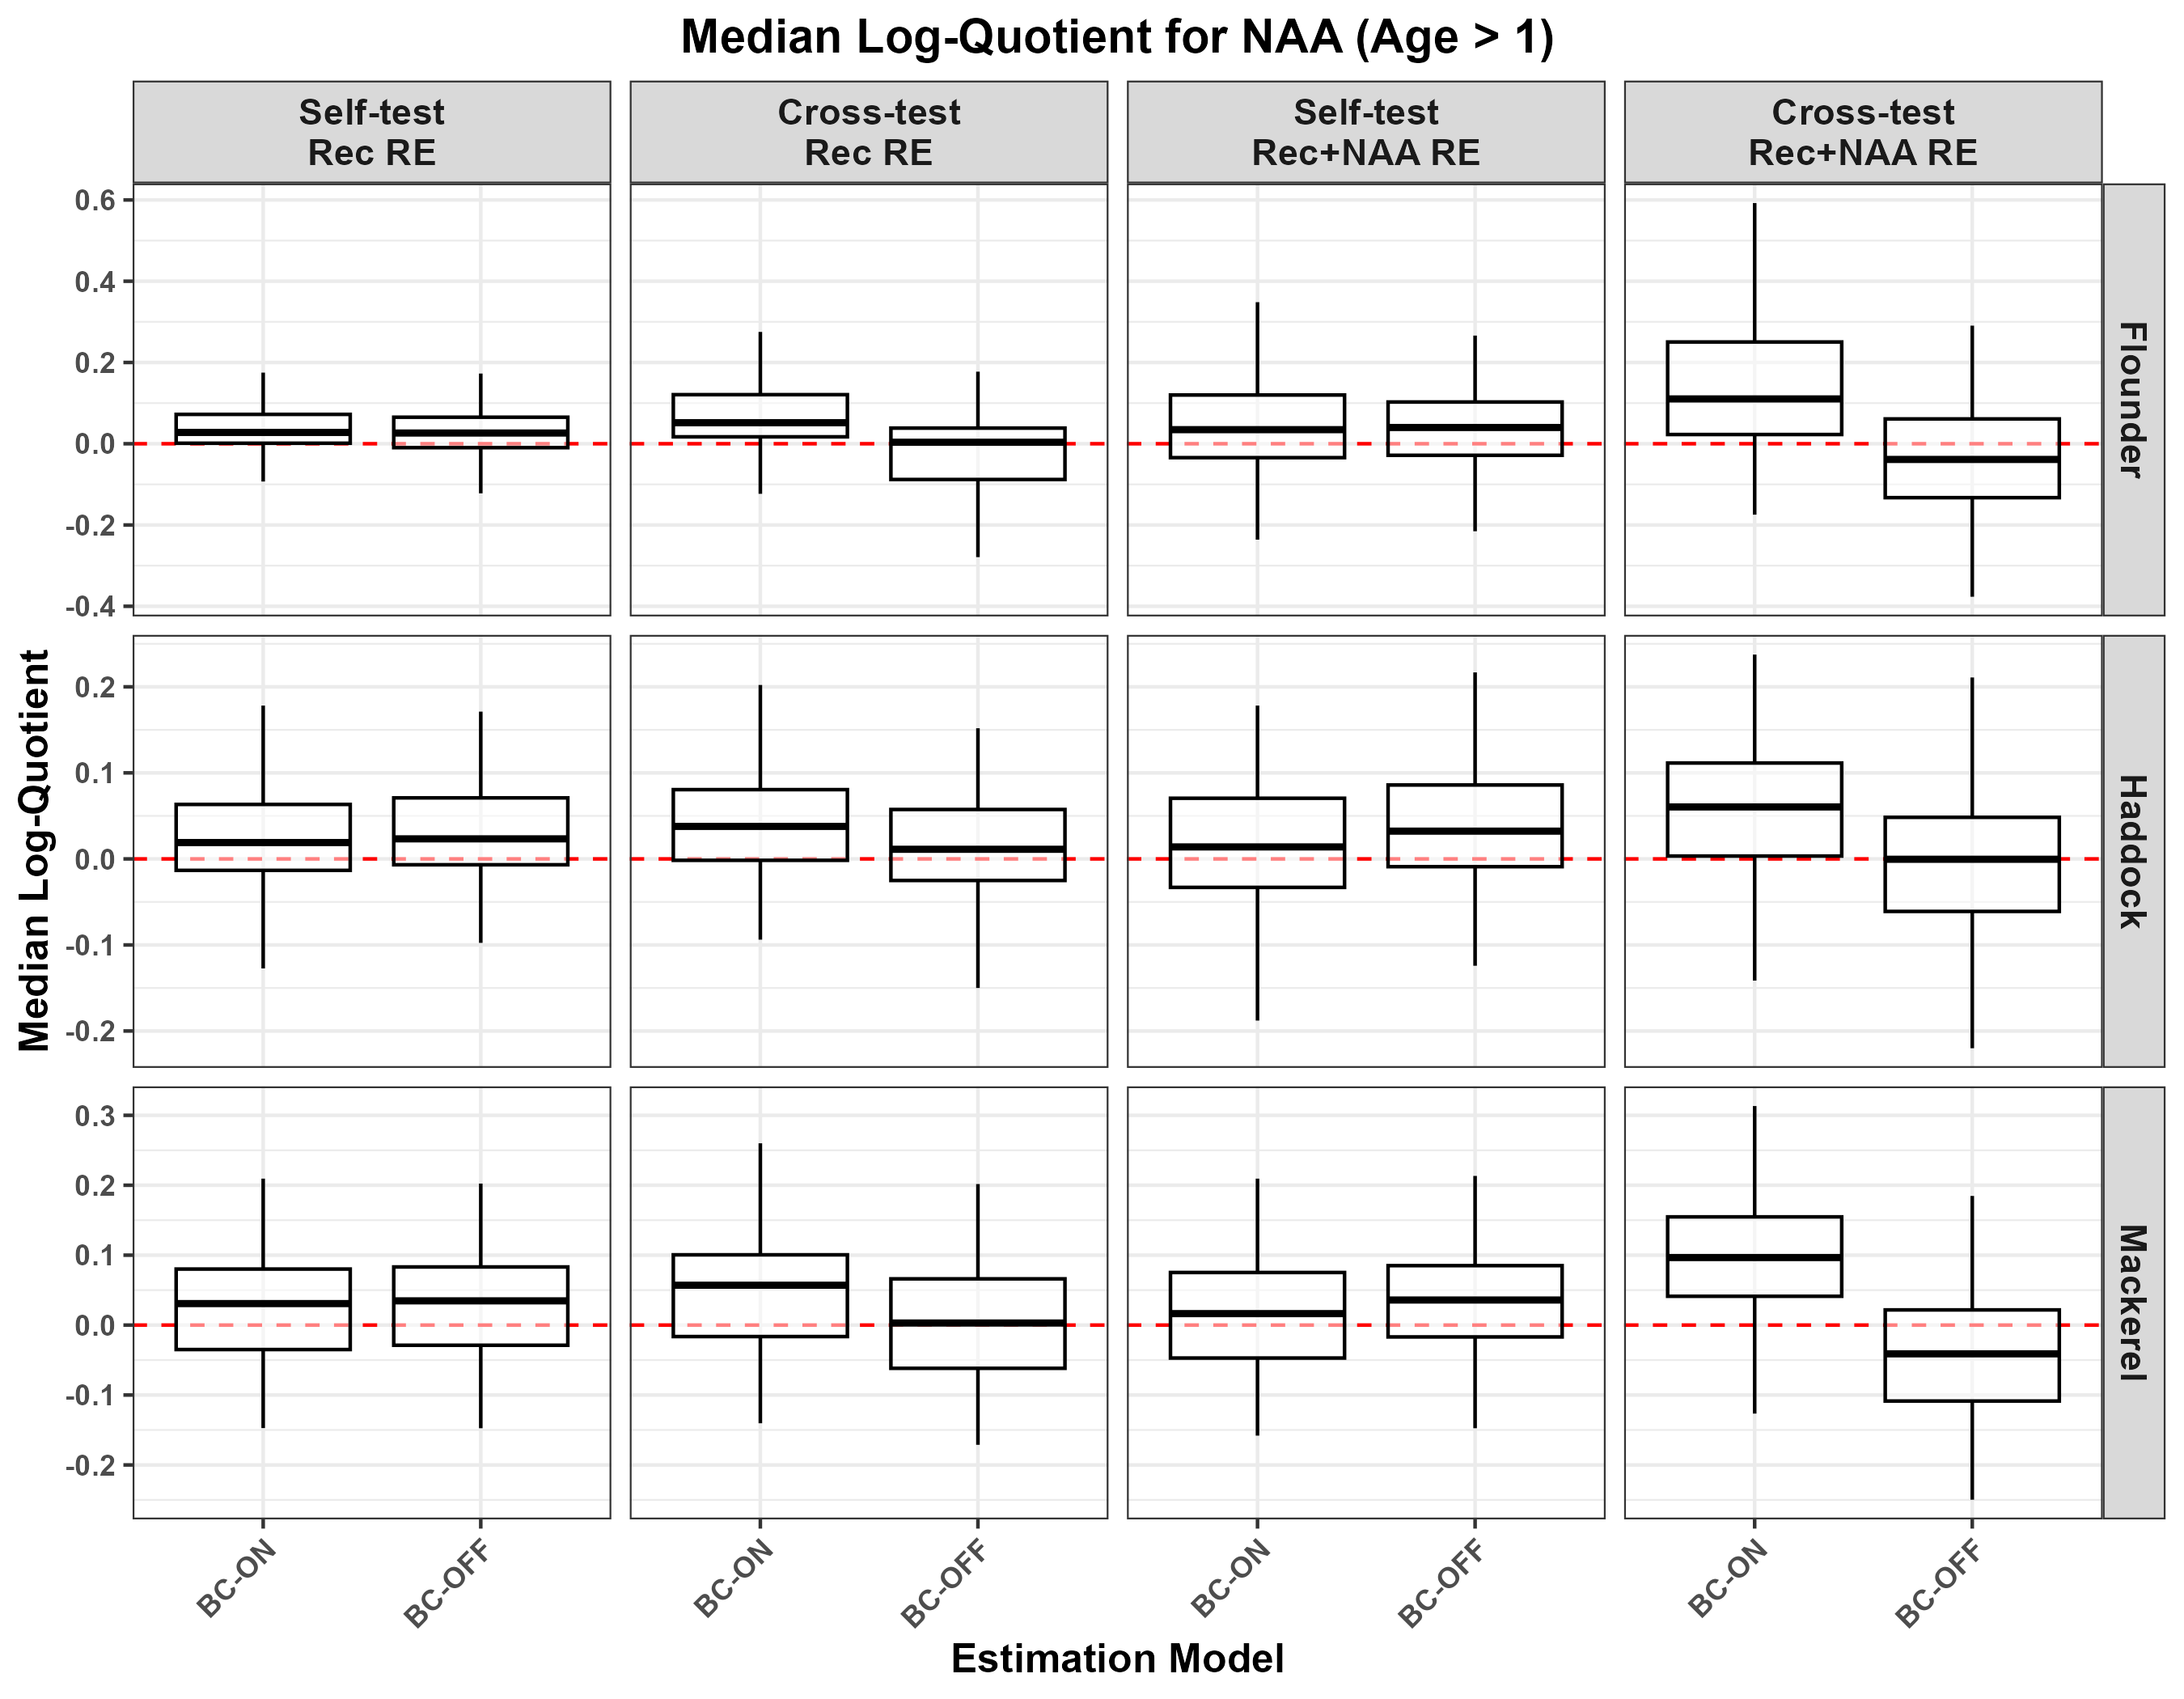
\includegraphics[width=\textwidth]{Revised_Figures&Tables/MdLQ_NAA.PNG}
    \caption{Median log-quotient (MdLQ) of $NAA$ calculated for self-tests and cross-tests. ``Rec RE'' and ``Rec+NAA RE'' in the top facet indicate operating models (OMs) with only recruitment random effects and both recruitment and $NAA$ random effects, respectively.}
    \label{fig:supp_NAA_MdLQ}
\end{figure}

\begin{figure}[H]
    \centering
    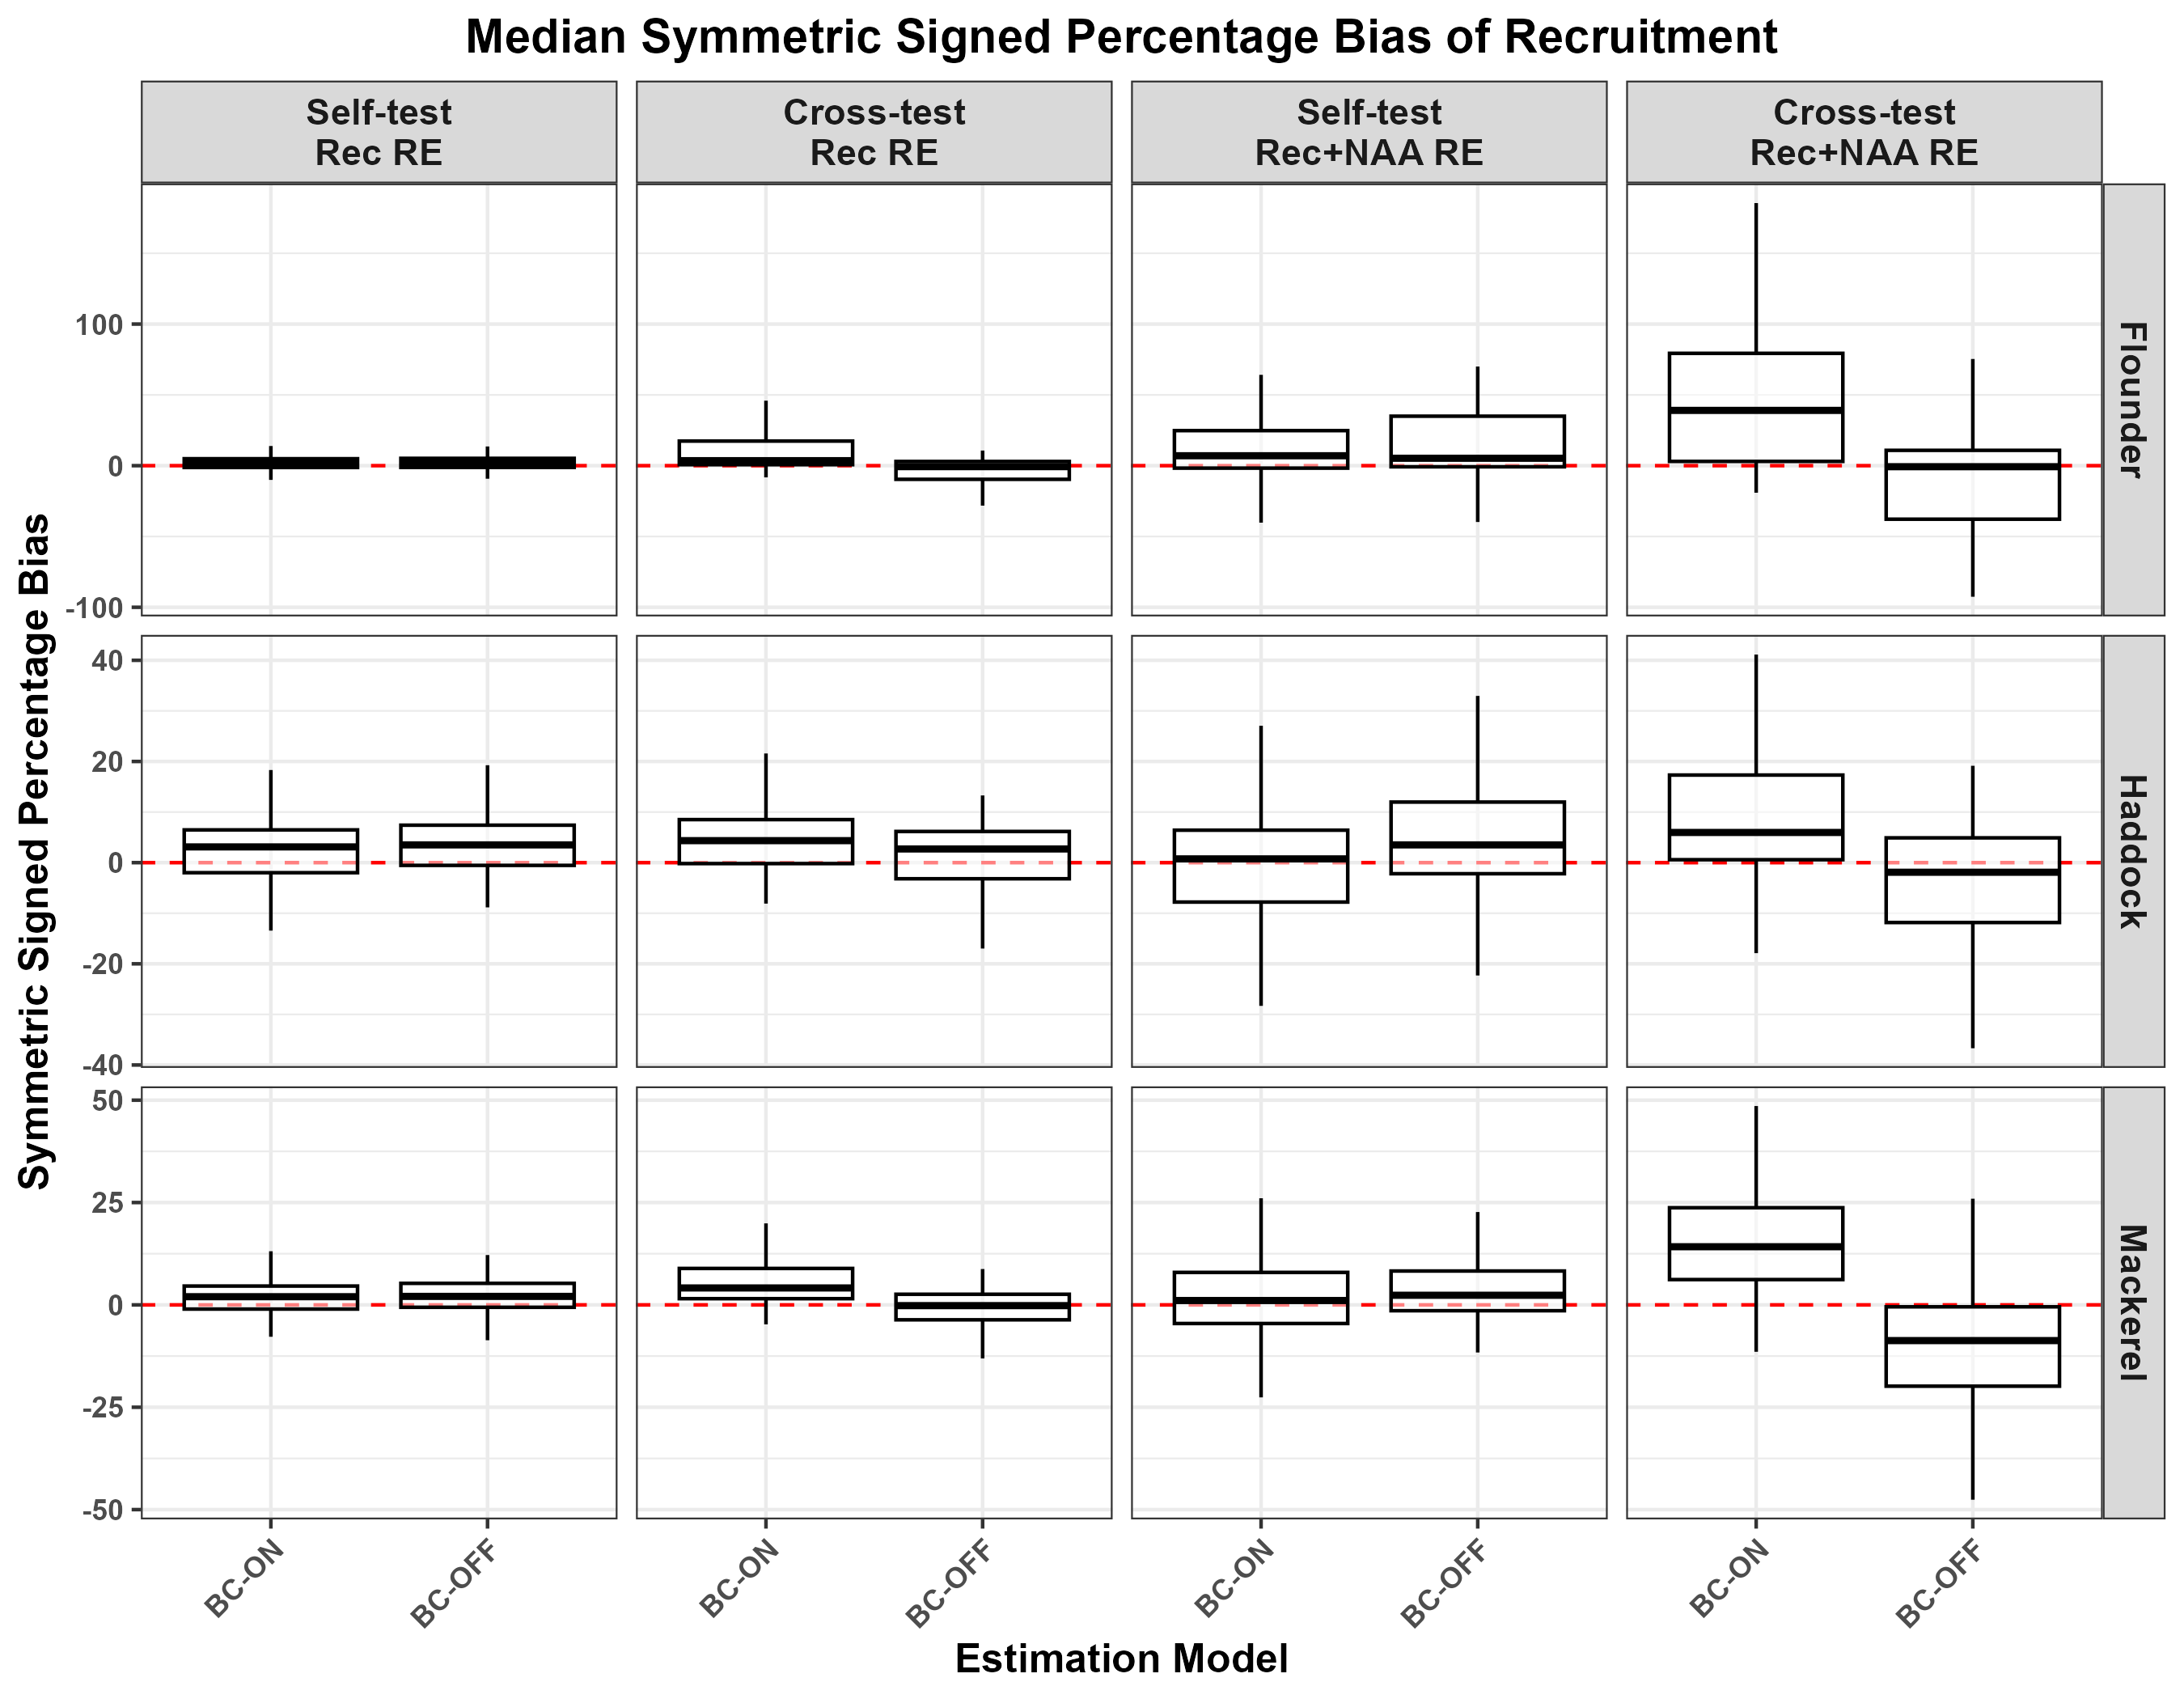
\includegraphics[width=\textwidth]{Revised_Figures&Tables/Median_Rec_SSPB.PNG}
    \caption{Median symmetric signed percentage bias (SSPB) of recruitment calculated for self-tests and cross-tests. ``Rec RE'' and ``Rec+NAA RE'' in the top facet indicate operating models (OMs) with only recruitment random effects and both recruitment and $NAA$ random effects, respectively.}
    \label{fig:supp_Rec_SSPB}
\end{figure}

\begin{figure}[H]
    \centering
    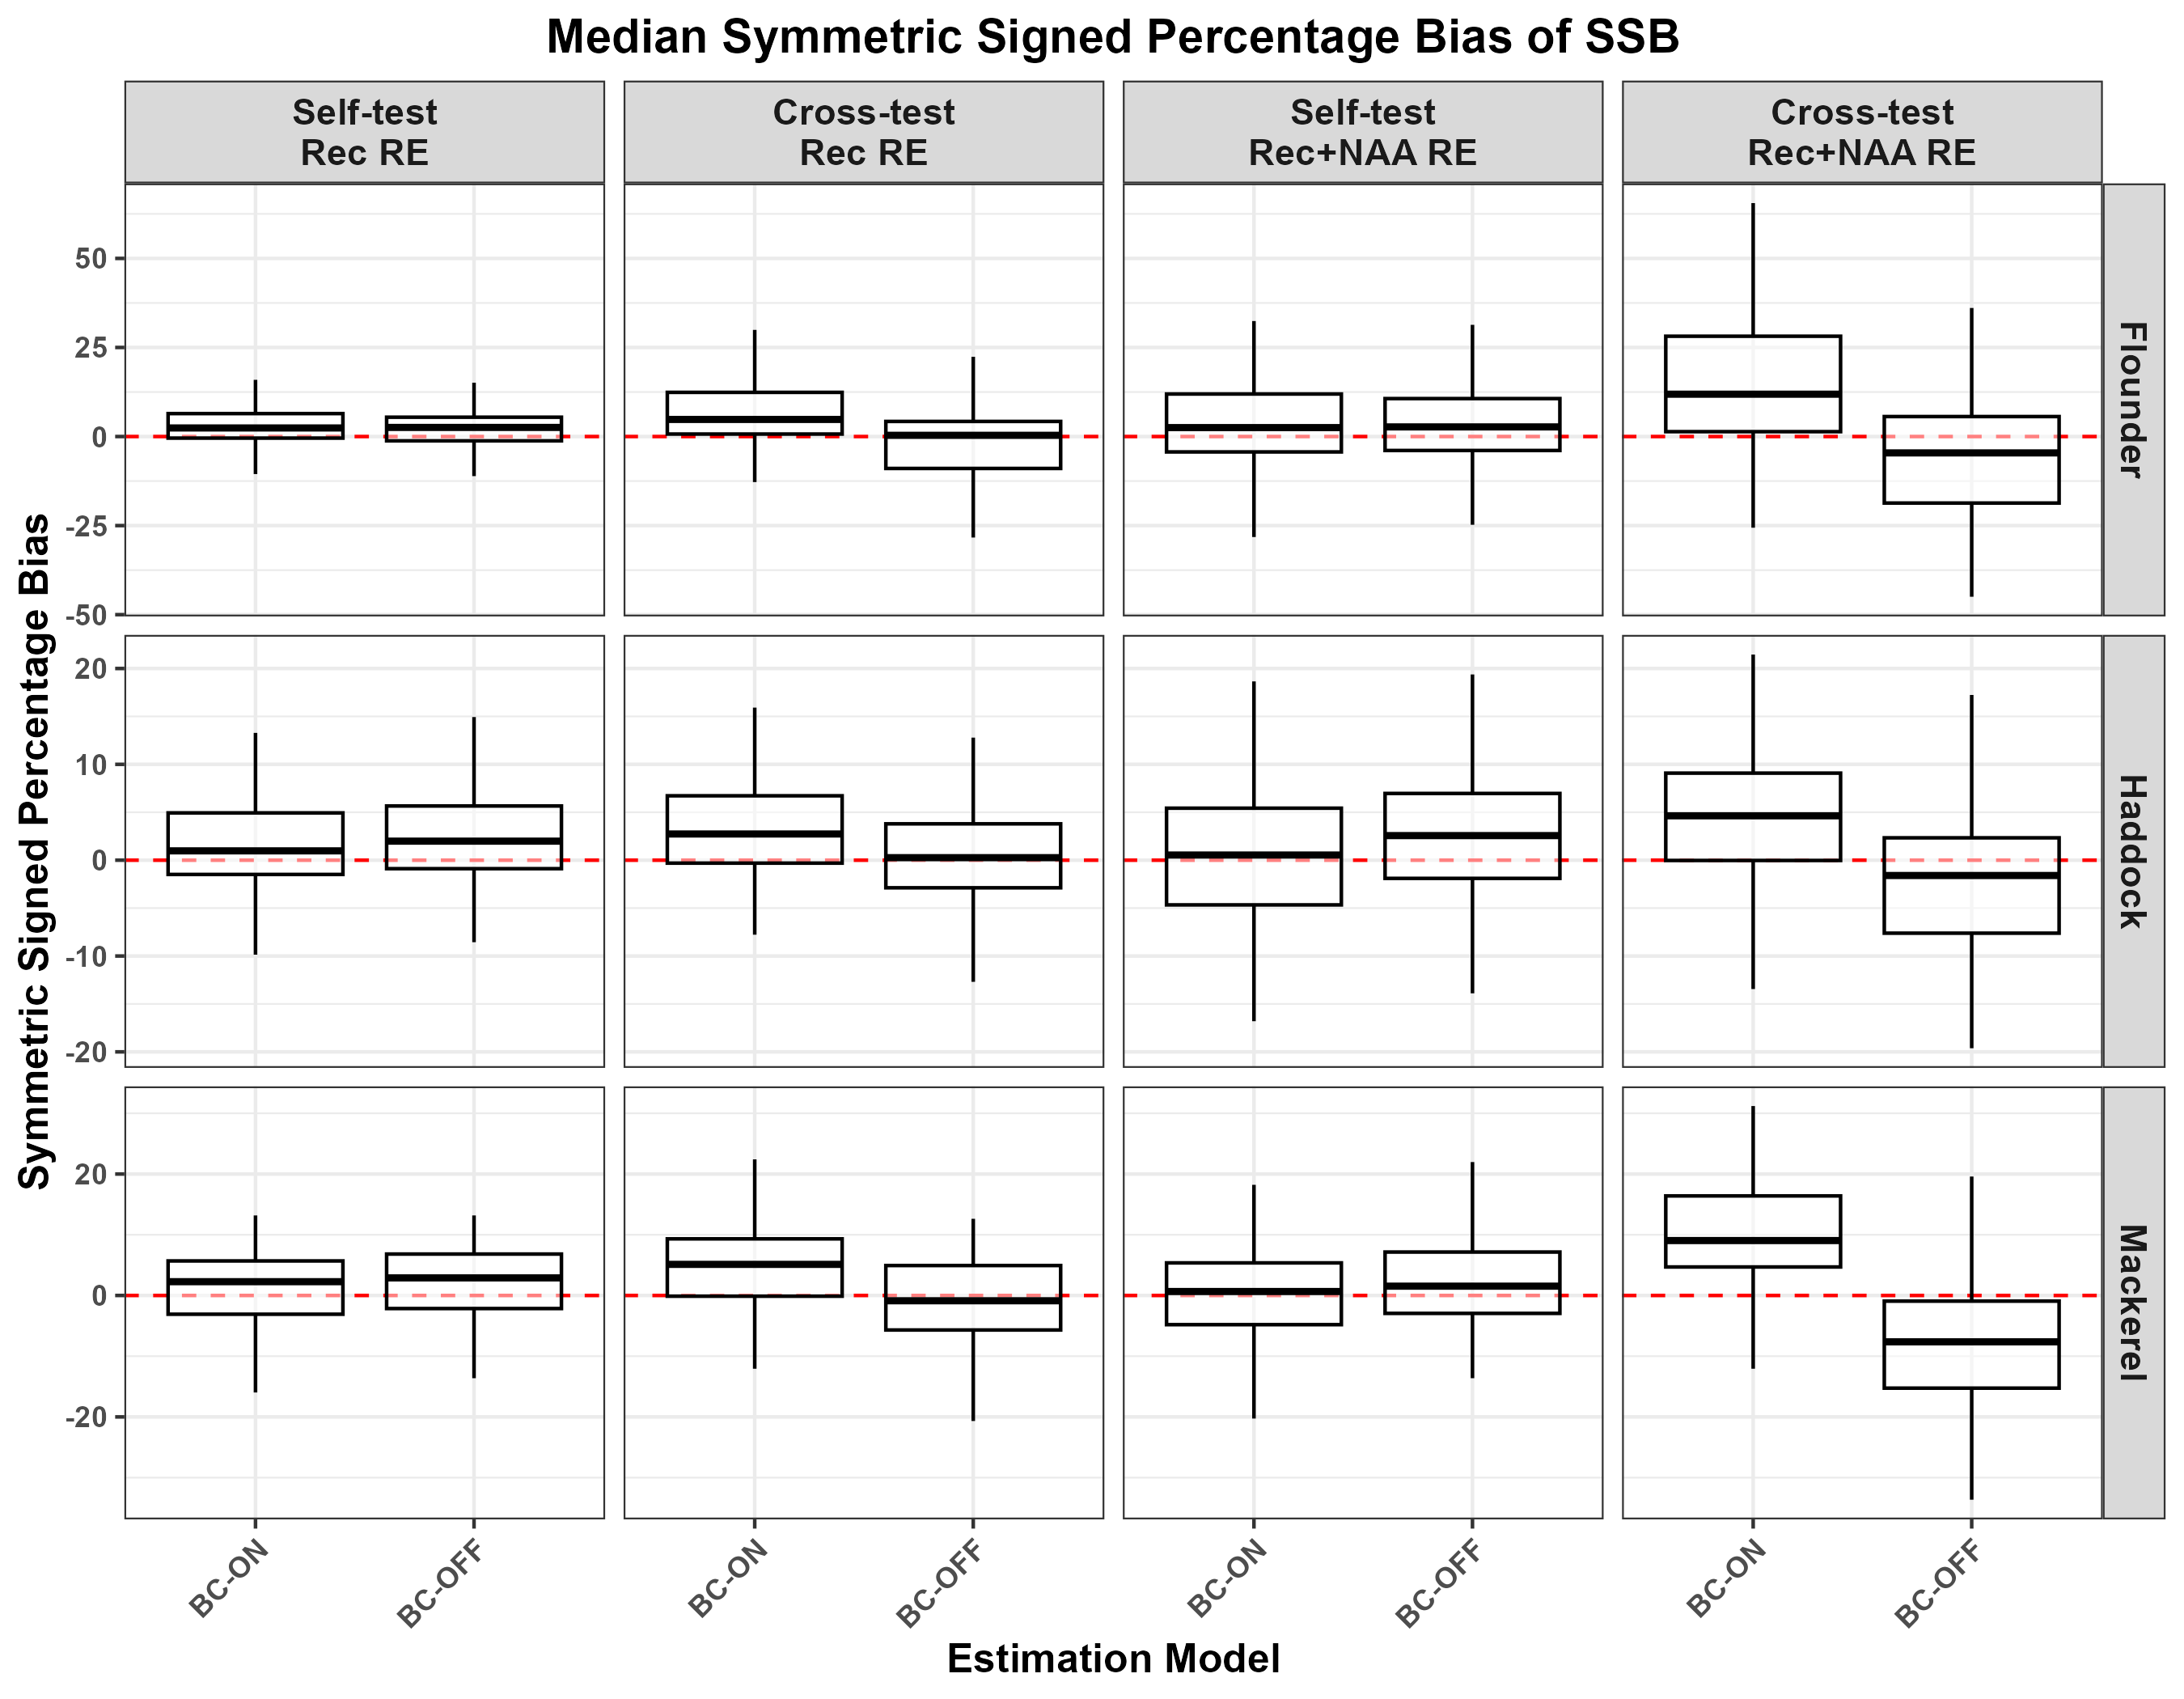
\includegraphics[width=\textwidth]{Revised_Figures&Tables/Median_SSB_SSPB.PNG}
    \caption{Median symmetric signed percentage bias (SSPB) of $SSB$ calculated for self-tests and cross-tests. ``Rec RE'' and ``Rec+NAA RE'' in the top facet indicate operating models (OMs) with only recruitment random effects and both recruitment and $NAA$ random effects, respectively.}
    \label{fig:supp_SSB_SSPB}
\end{figure}

\begin{figure}[H]
    \centering
    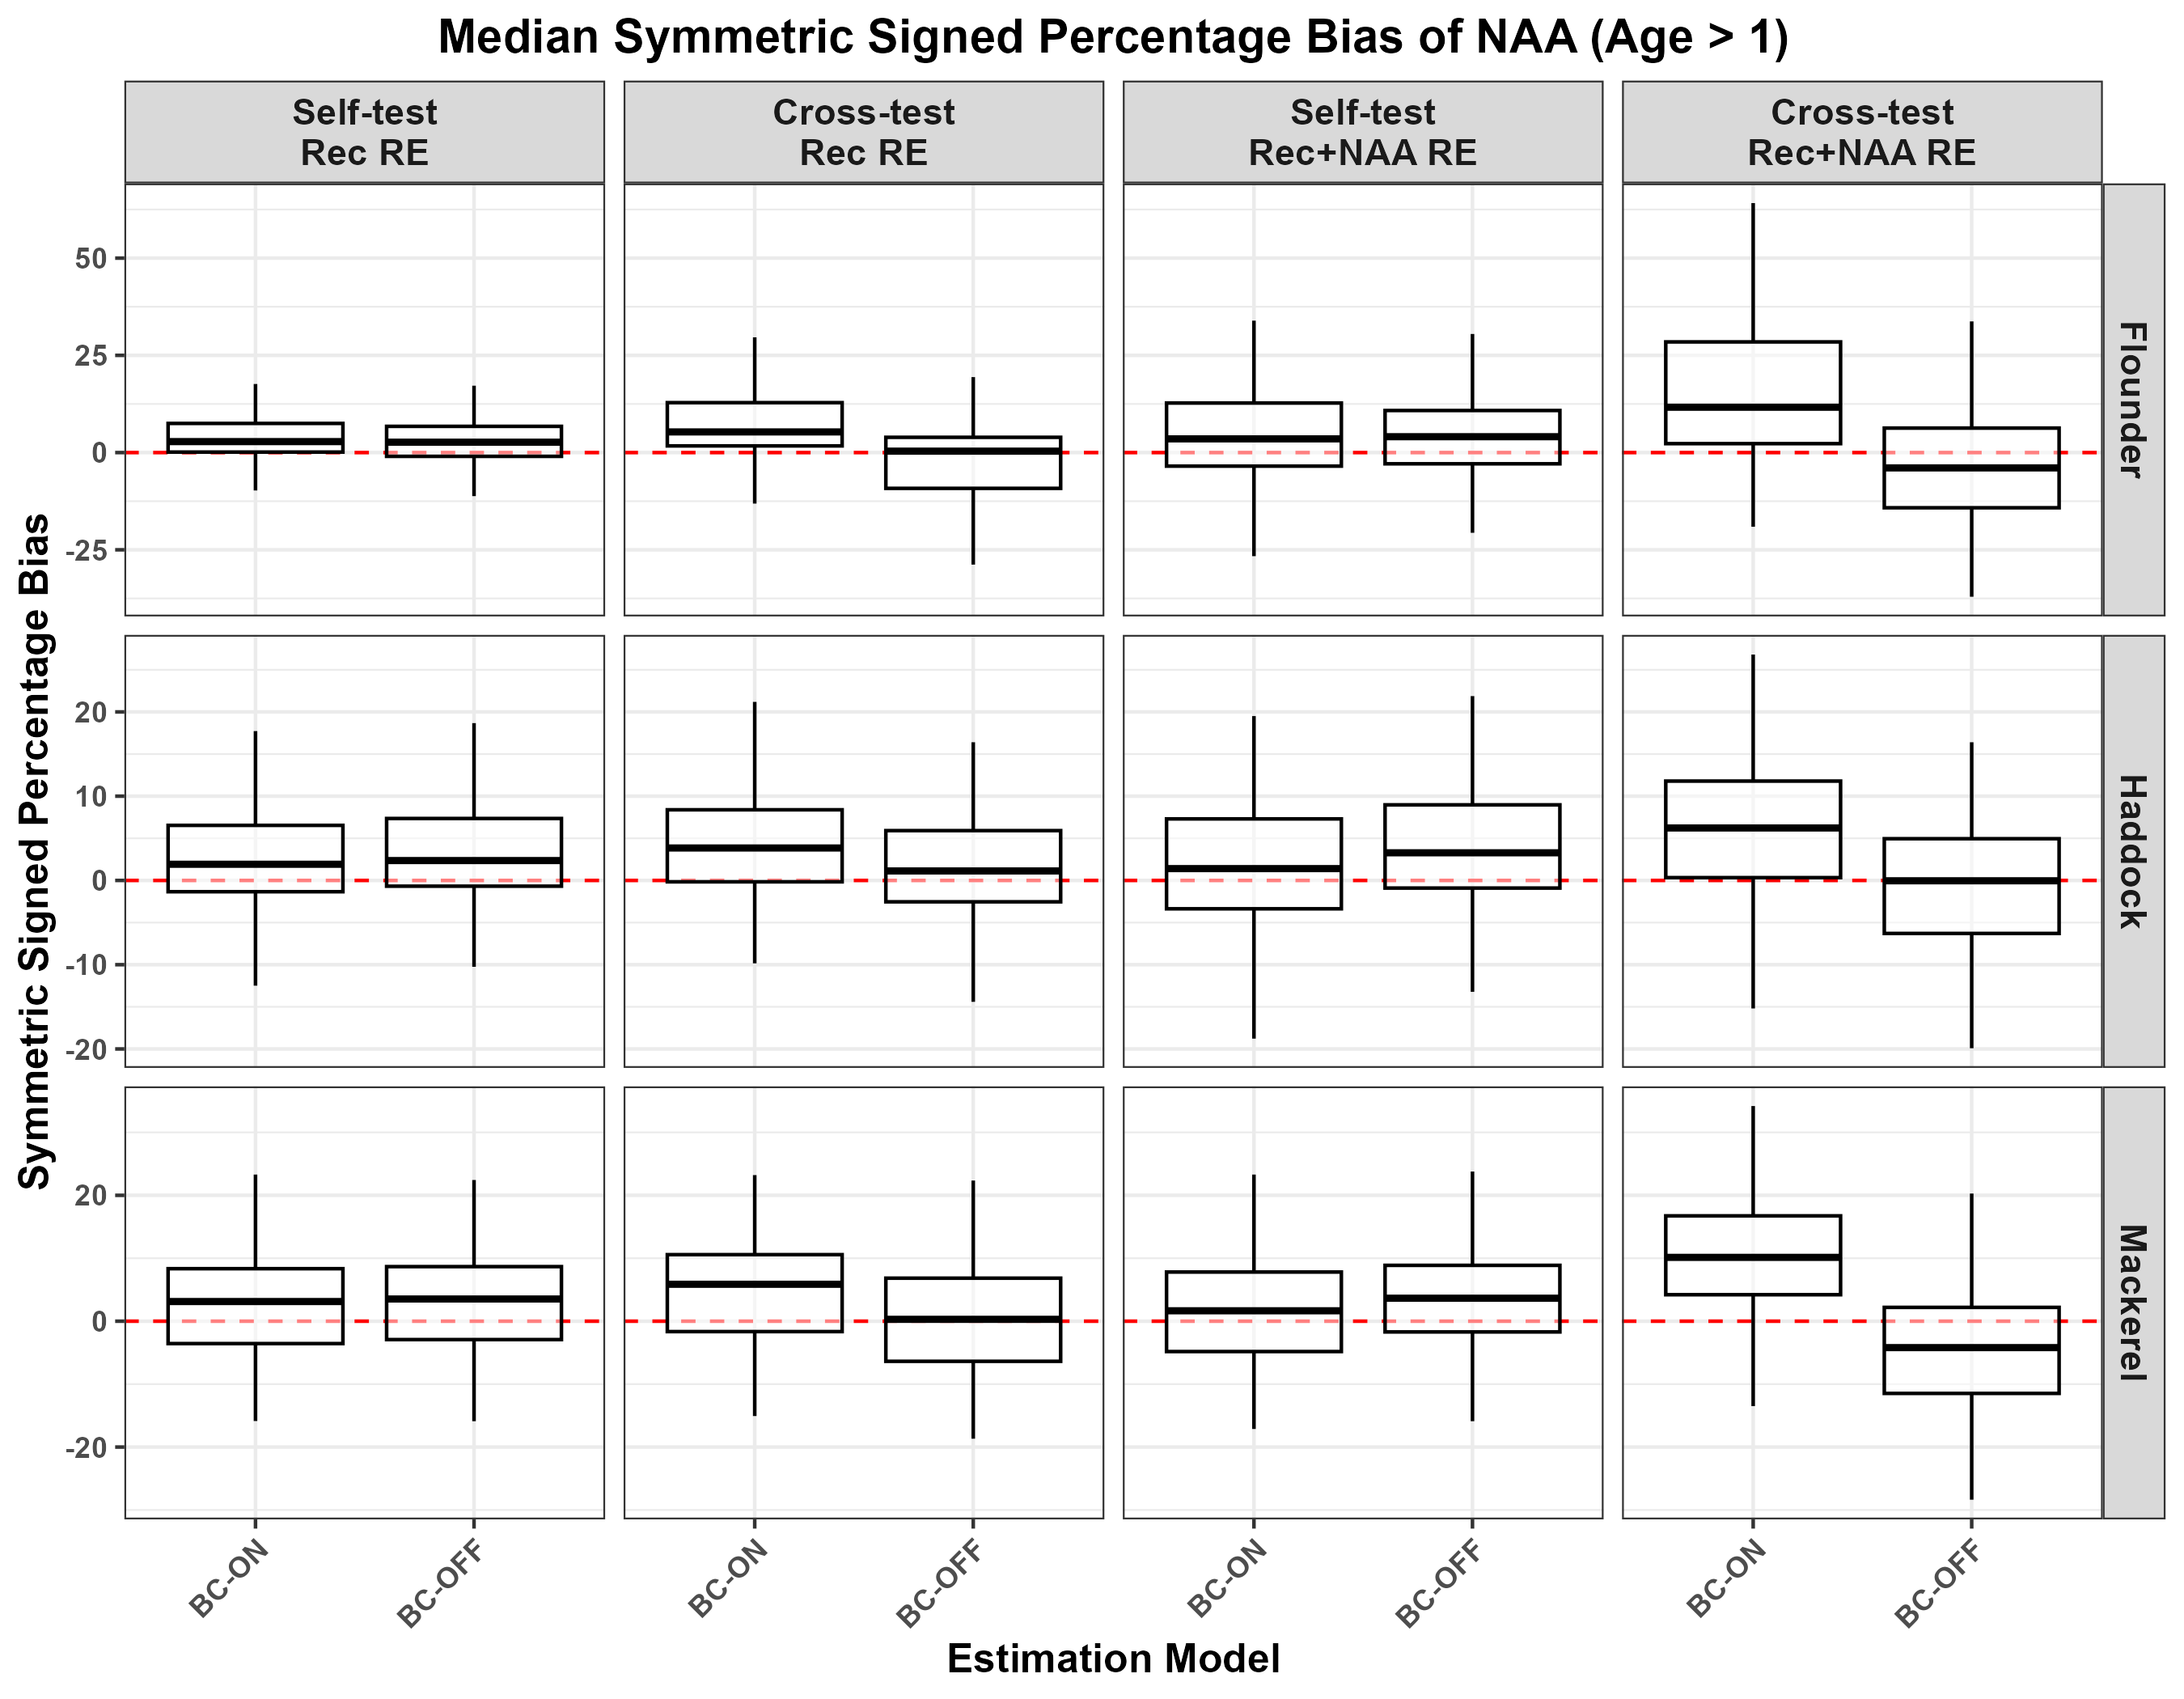
\includegraphics[width=\textwidth]{Revised_Figures&Tables/Median_NAA_SSPB.PNG}
    \caption{Median symmetric signed percentage bias (SSPB) of $NAA$ calculated for self-tests and cross-tests. ``Rec RE'' and ``Rec+NAA RE'' in the top facet indicate operating models (OMs) with only recruitment random effects and both recruitment and $NAA$ random effects, respectively.}
    \label{fig:supp_NAA_SSPB}
\end{figure}

\begin{figure}[H]
\centering
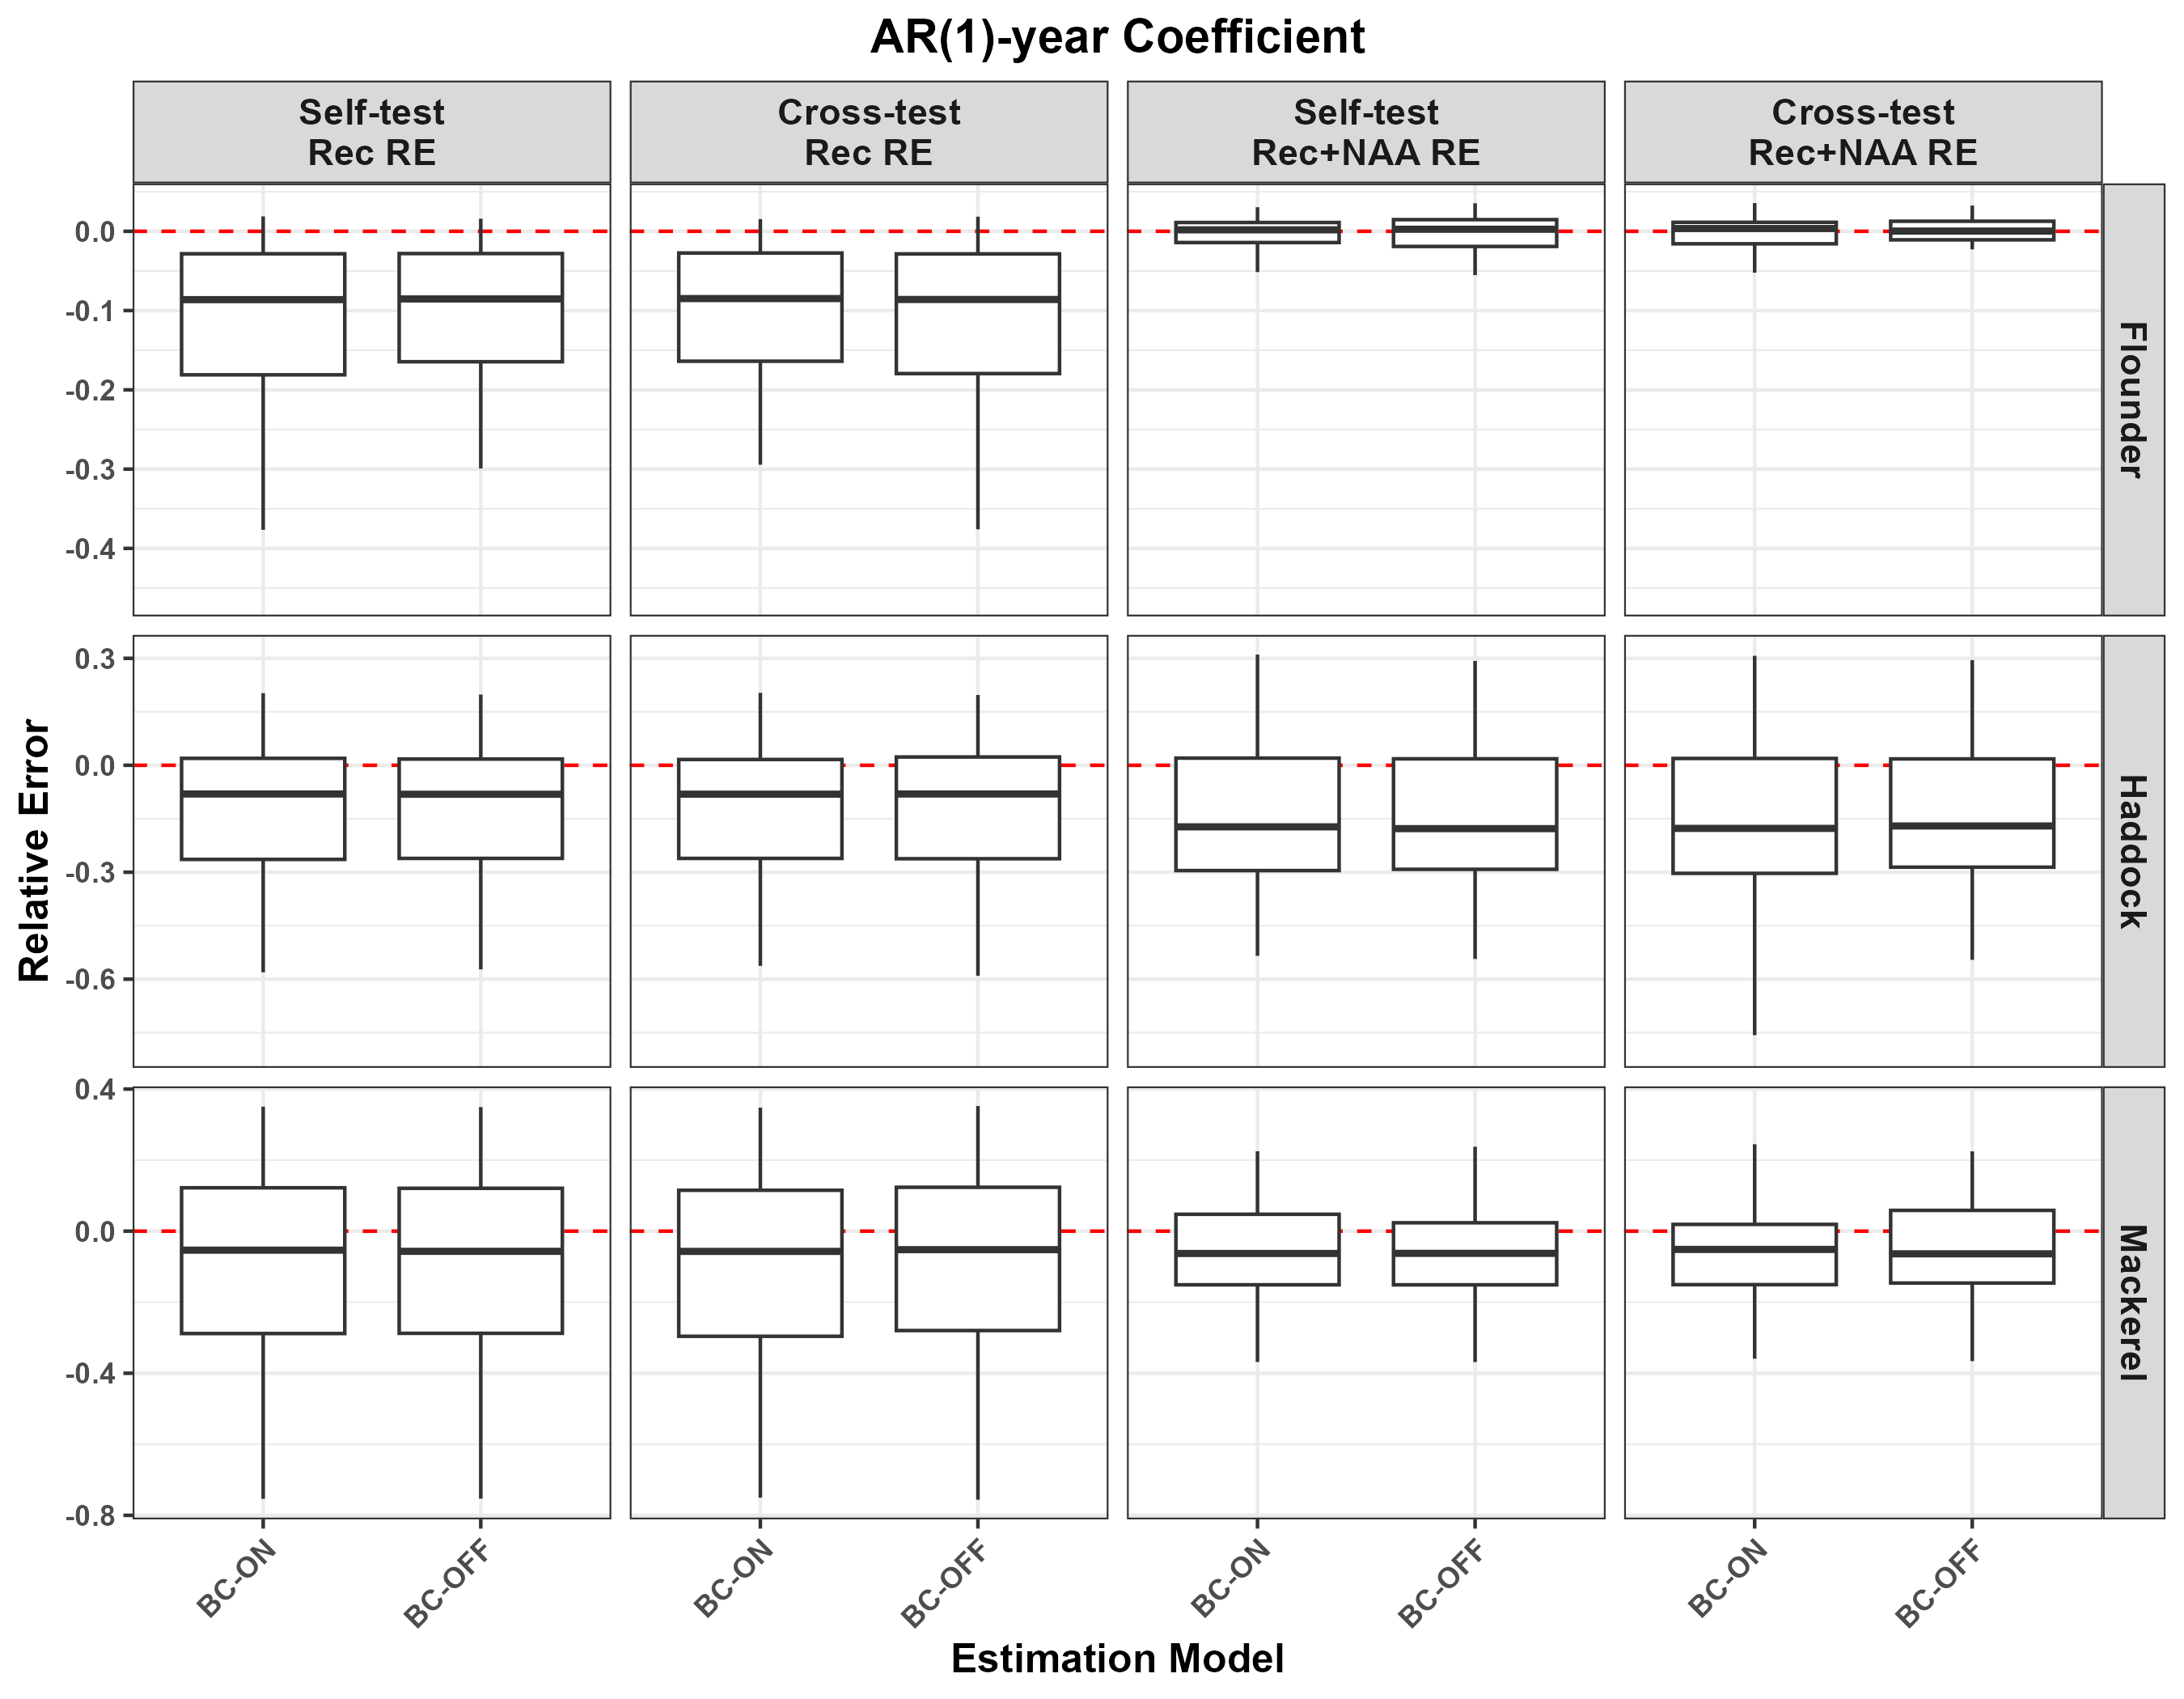
\includegraphics[width=\textwidth]{Revised_Figures&Tables/Rho.PNG}
\caption{Relative error of AR(1)-year coefficient calculated for self-tests and cross-tests. ``Rec RE'' and ``Rec+NAA RE'' in the top facet indicate operating models (OMs) with only recruitment random effects and both recruitment and $NAA$ random effects, respectively.}
\label{fig:supp_ar1}
\end{figure}

\begin{figure}[H]
    \centering
    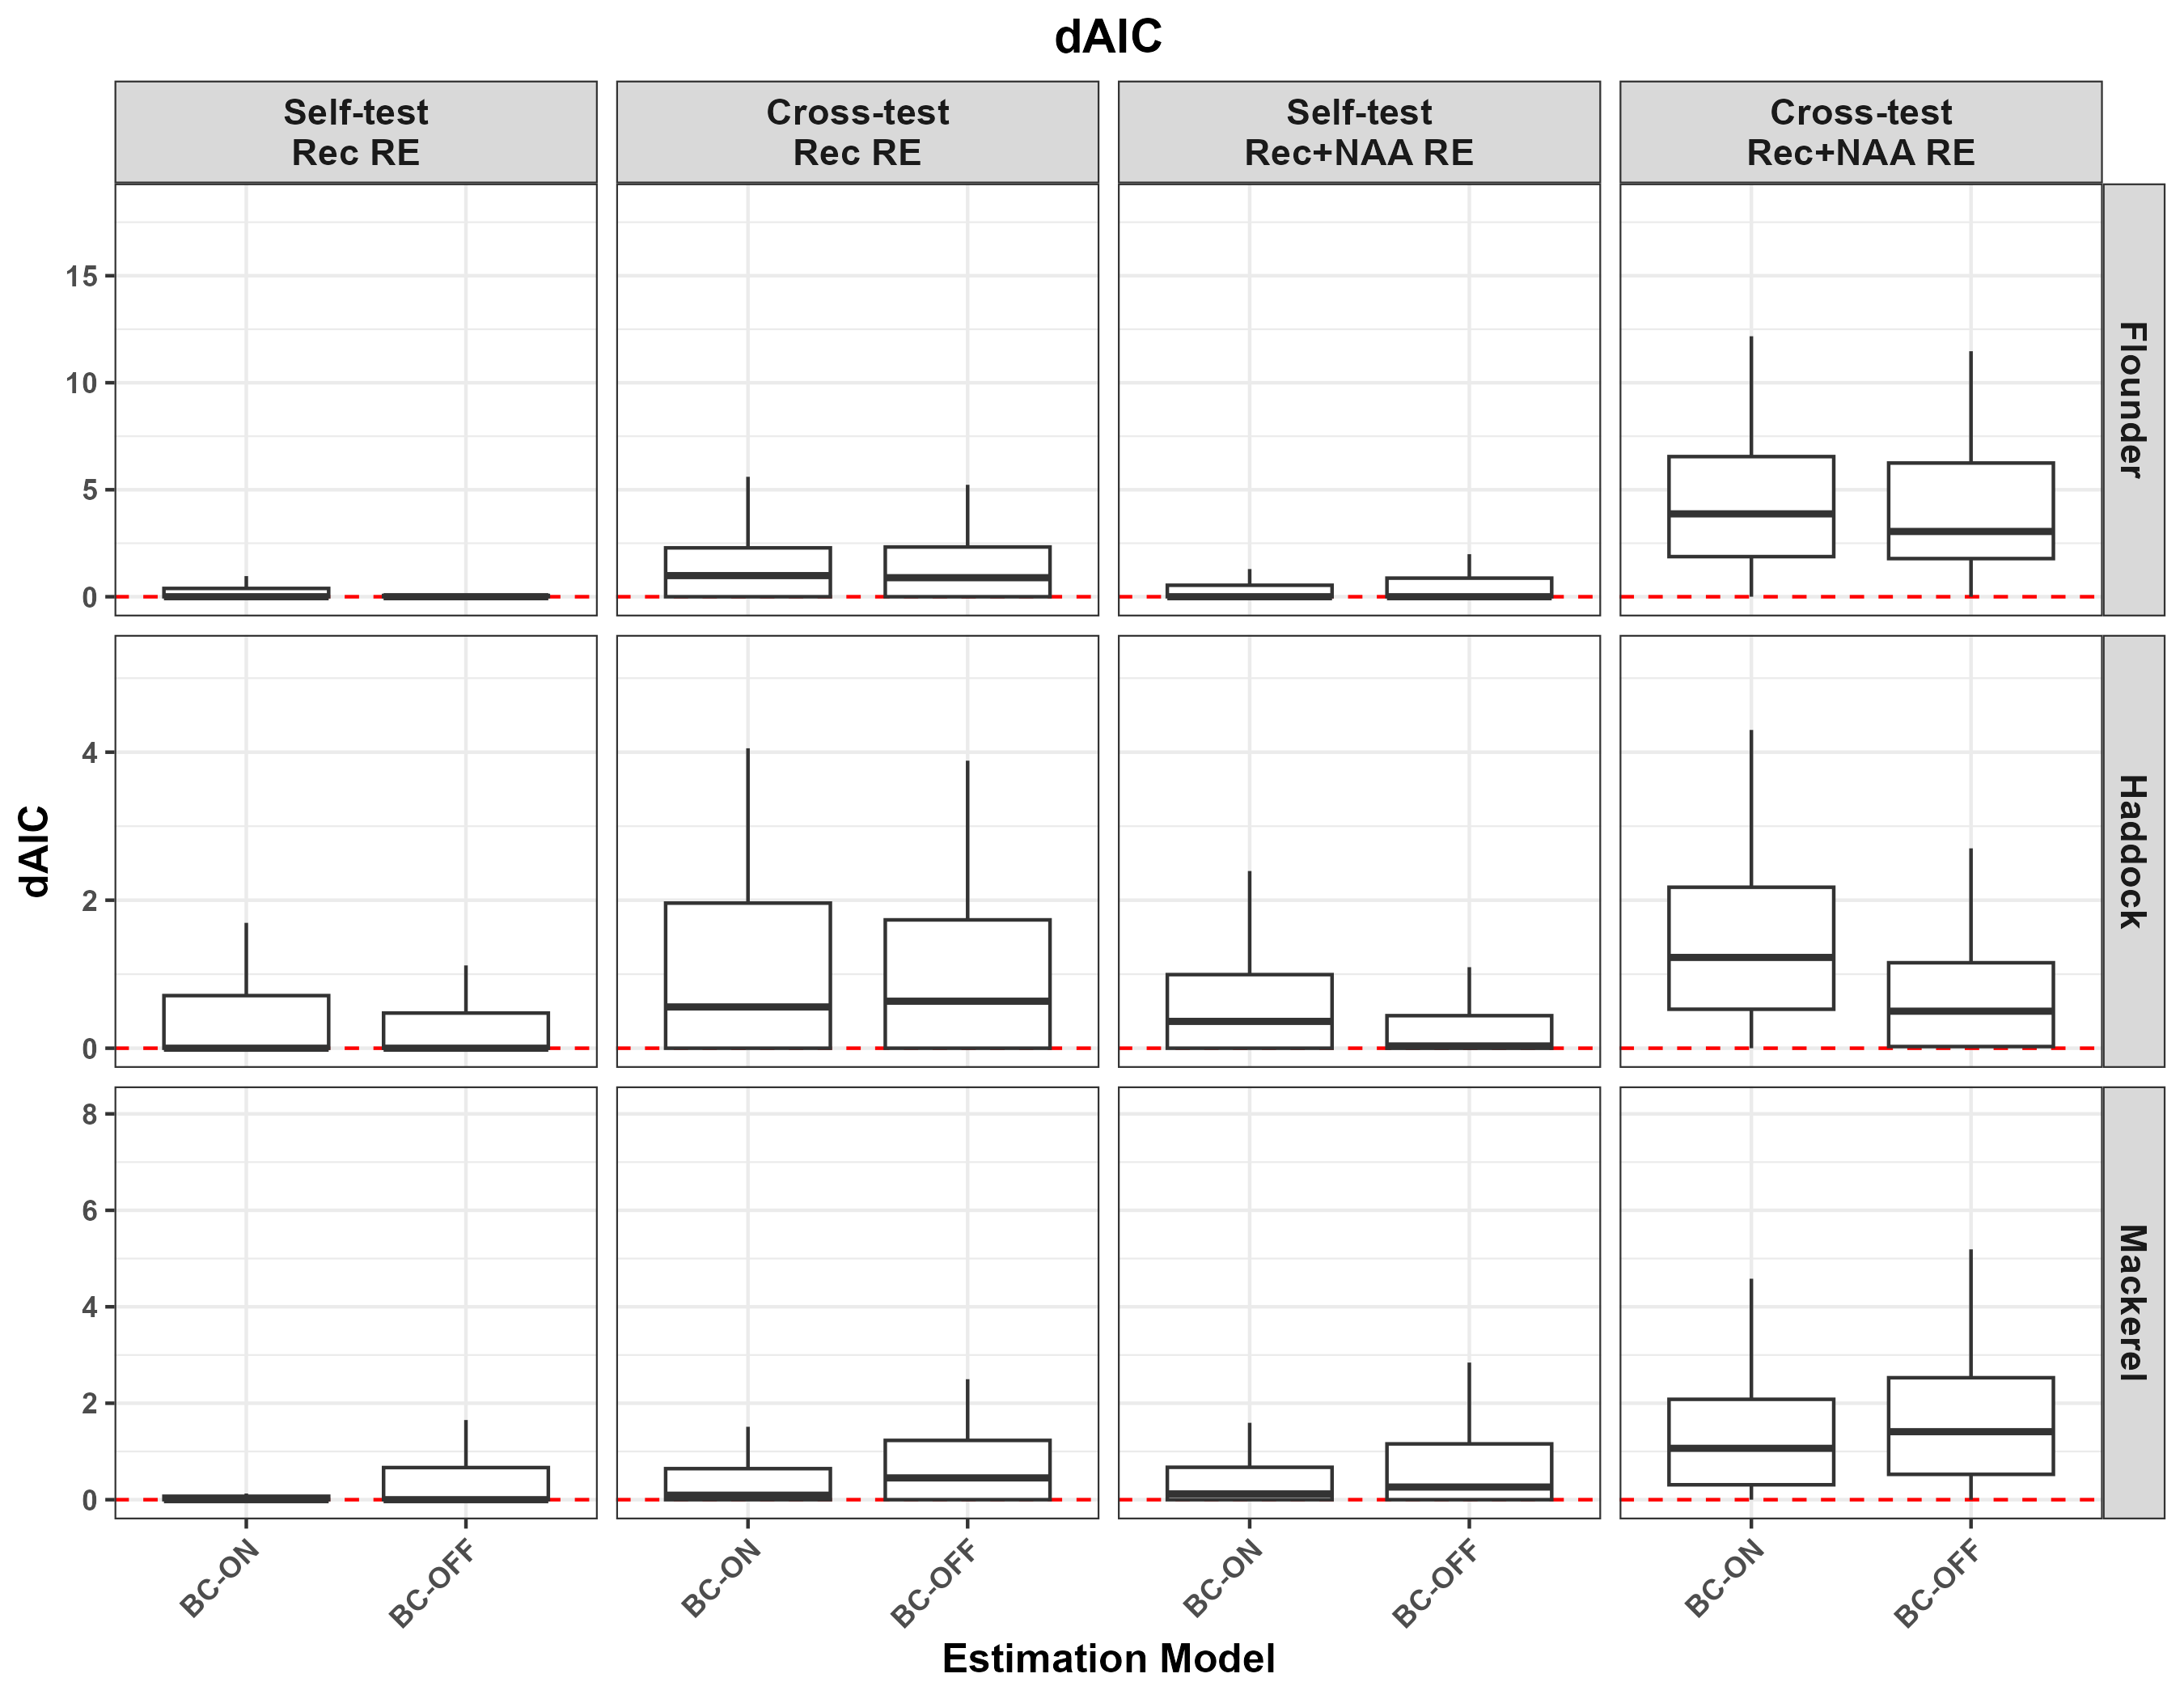
\includegraphics[width=\textwidth]{Revised_Figures&Tables/dAIC.PNG}
    \caption{dAIC calculated for self-tests and cross-tests. ``Rec RE'' and ``Rec+NAA RE'' in the top facet indicate operating models (OMs) with only recruitment random effects and both recruitment and $NAA$ random effects, respectively.}
    \label{fig:supp_dAIC}
\end{figure}

\begin{figure}[H]
    \centering
    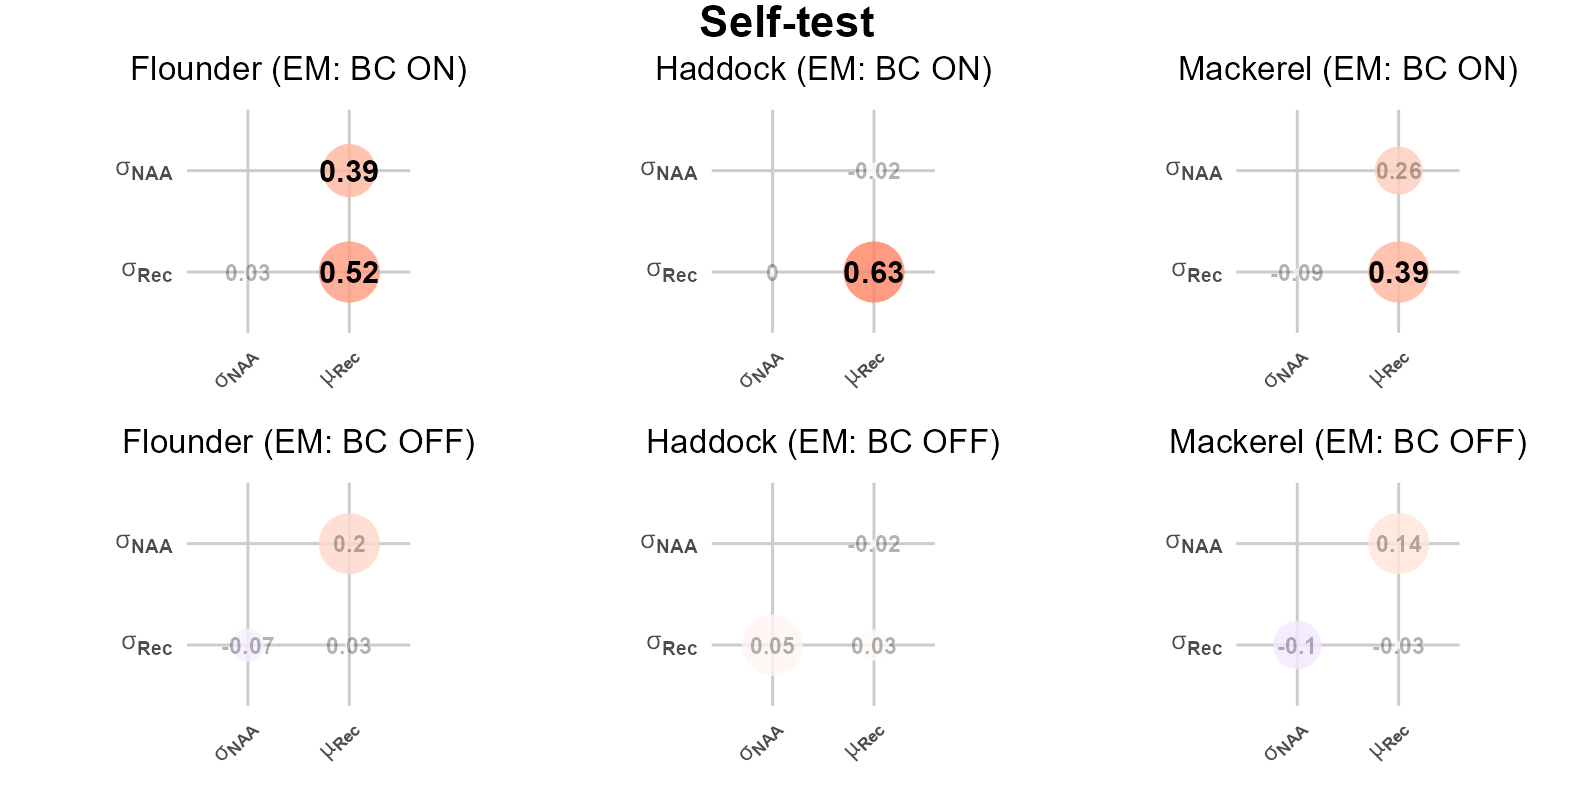
\includegraphics[width=\textwidth]{Revised_Figures&Tables/Correlation_plot_NAA_iid.PNG}
    \caption{Correlation plot for the OM with both recruitment and $NAA$ treated as IID random effects. The correlations were calculated from self-tests, where the EM had the same bias correction as the operating model (OM). Correlations in \textbf{bold} indicate statistically significant values (p-value < 0.05).}
    \label{fig:supp_Cor_NAA_iid}
\end{figure}

\begin{figure}[H]
    \centering
    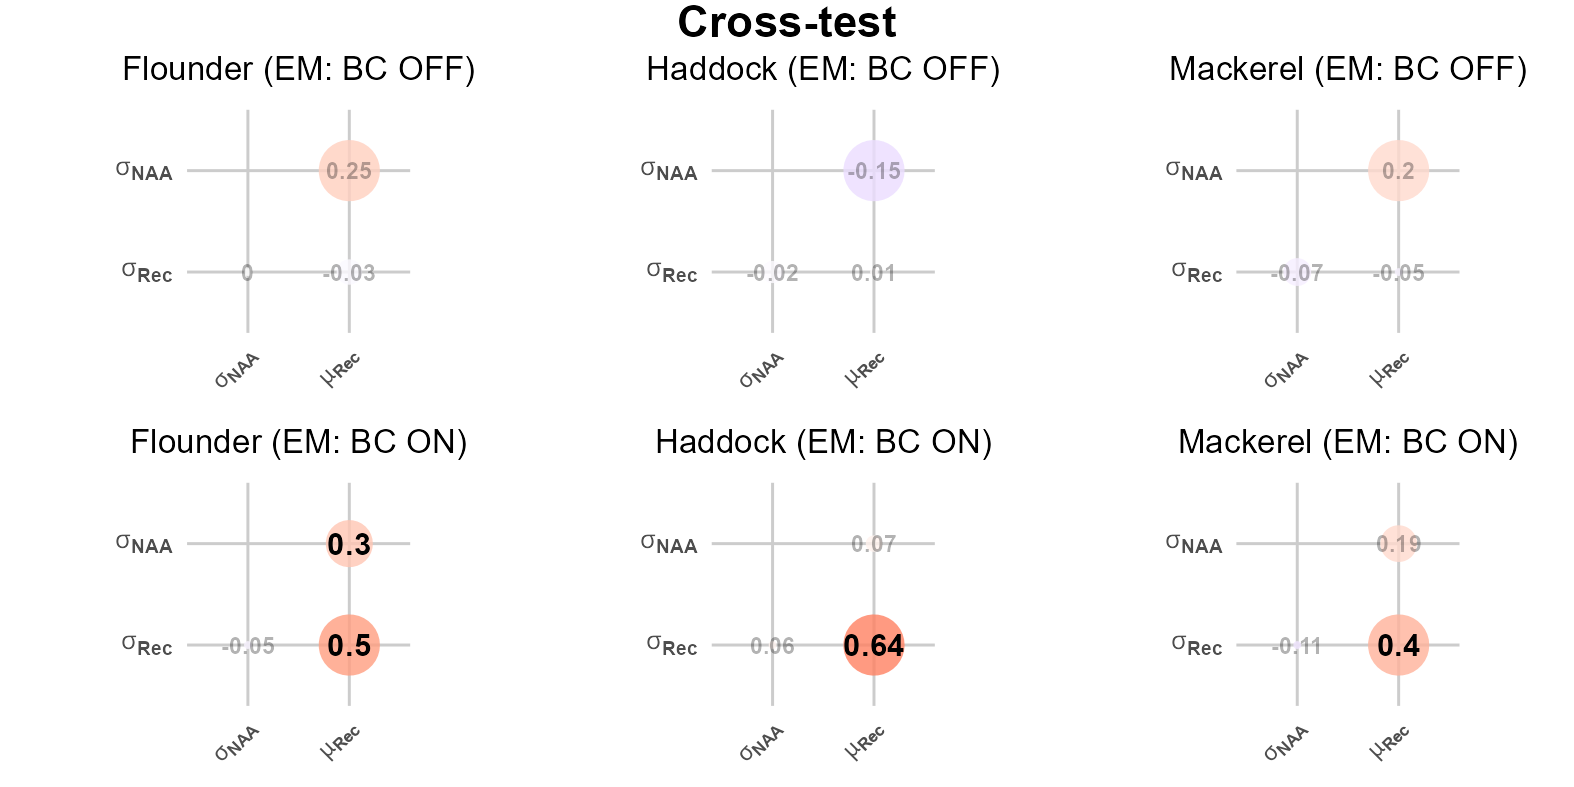
\includegraphics[width=\textwidth]{Revised_Figures&Tables/Correlation_plot_NAA_iid_mismatch.PNG}
    \caption{Correlation plot for the OM with both recruitment and $NAA$ treated as IID random effects. The correlations were calculated from cross-tests, where the EM had a different bias correction than the operating model (OM). Correlations in \textbf{bold} indicate statistically significant values (p-value < 0.05).}
    \label{fig:supp_Cor_NAA_iid_mis}
\end{figure}

\begin{figure}[H]
\centering
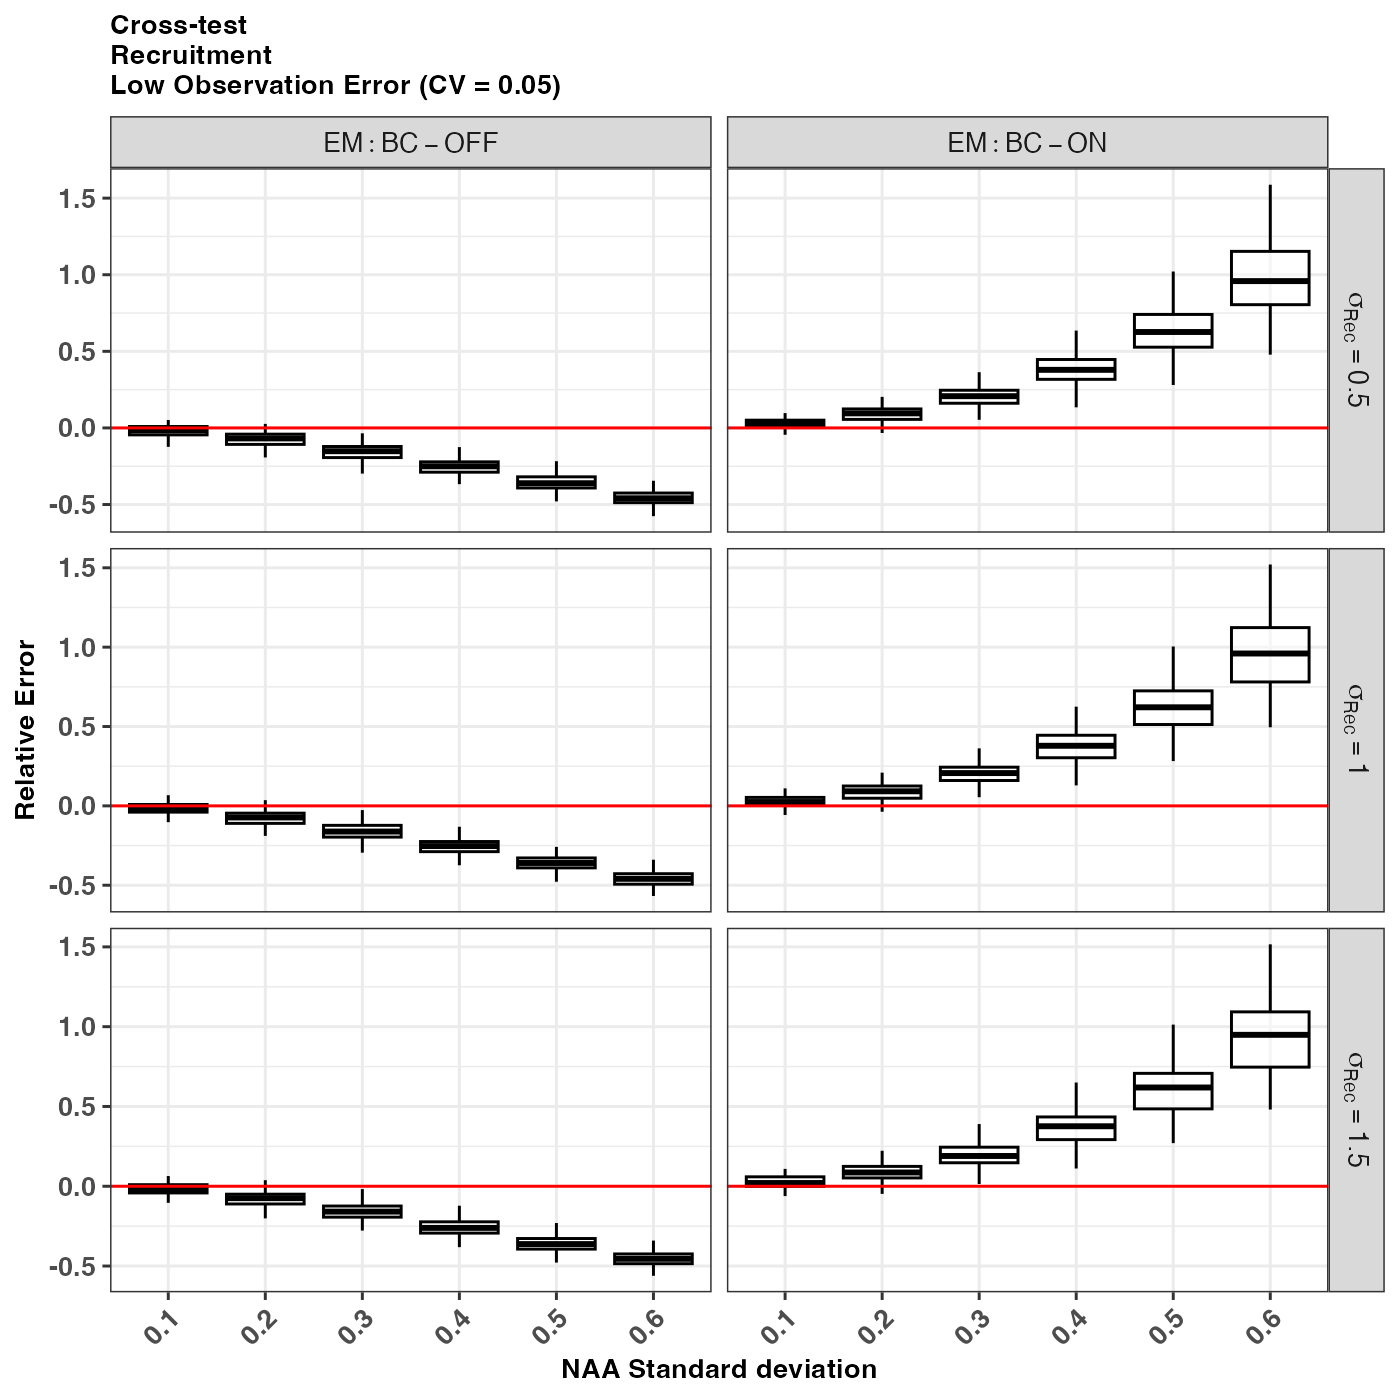
\includegraphics[width=\textwidth]{Revised_Figures&Tables/Recruitment_low_cross_RE.PNG}
\caption{Relative errors of recruitment estimates summarized from 50 realizations for each scenario. Two operating models (OMs) (with bias correction applied or omitted for both processes and observations) for Gulf of Maine (GoM) haddock with both recruitment and $NAA$ IID random effects (see Table S2) were used to conduct simulation-estimation experiments. The study evaluated the effects of recruitment variability ($\sigma_{Rec}$ = 0.5, 1, 1.5) and $NAA$ variability ($\sigma_{NAA}$ = 0.1, 0.2, ... 0.6) in a factorial design through self-tests and cross-tests. To isolate the impact of observation error, the coefficient of variation (CV) for observations was set to 0.05.}
\label{fig:supp_Recruitment_low_cross_RE}
\end{figure}

\begin{figure}[H]
\centering
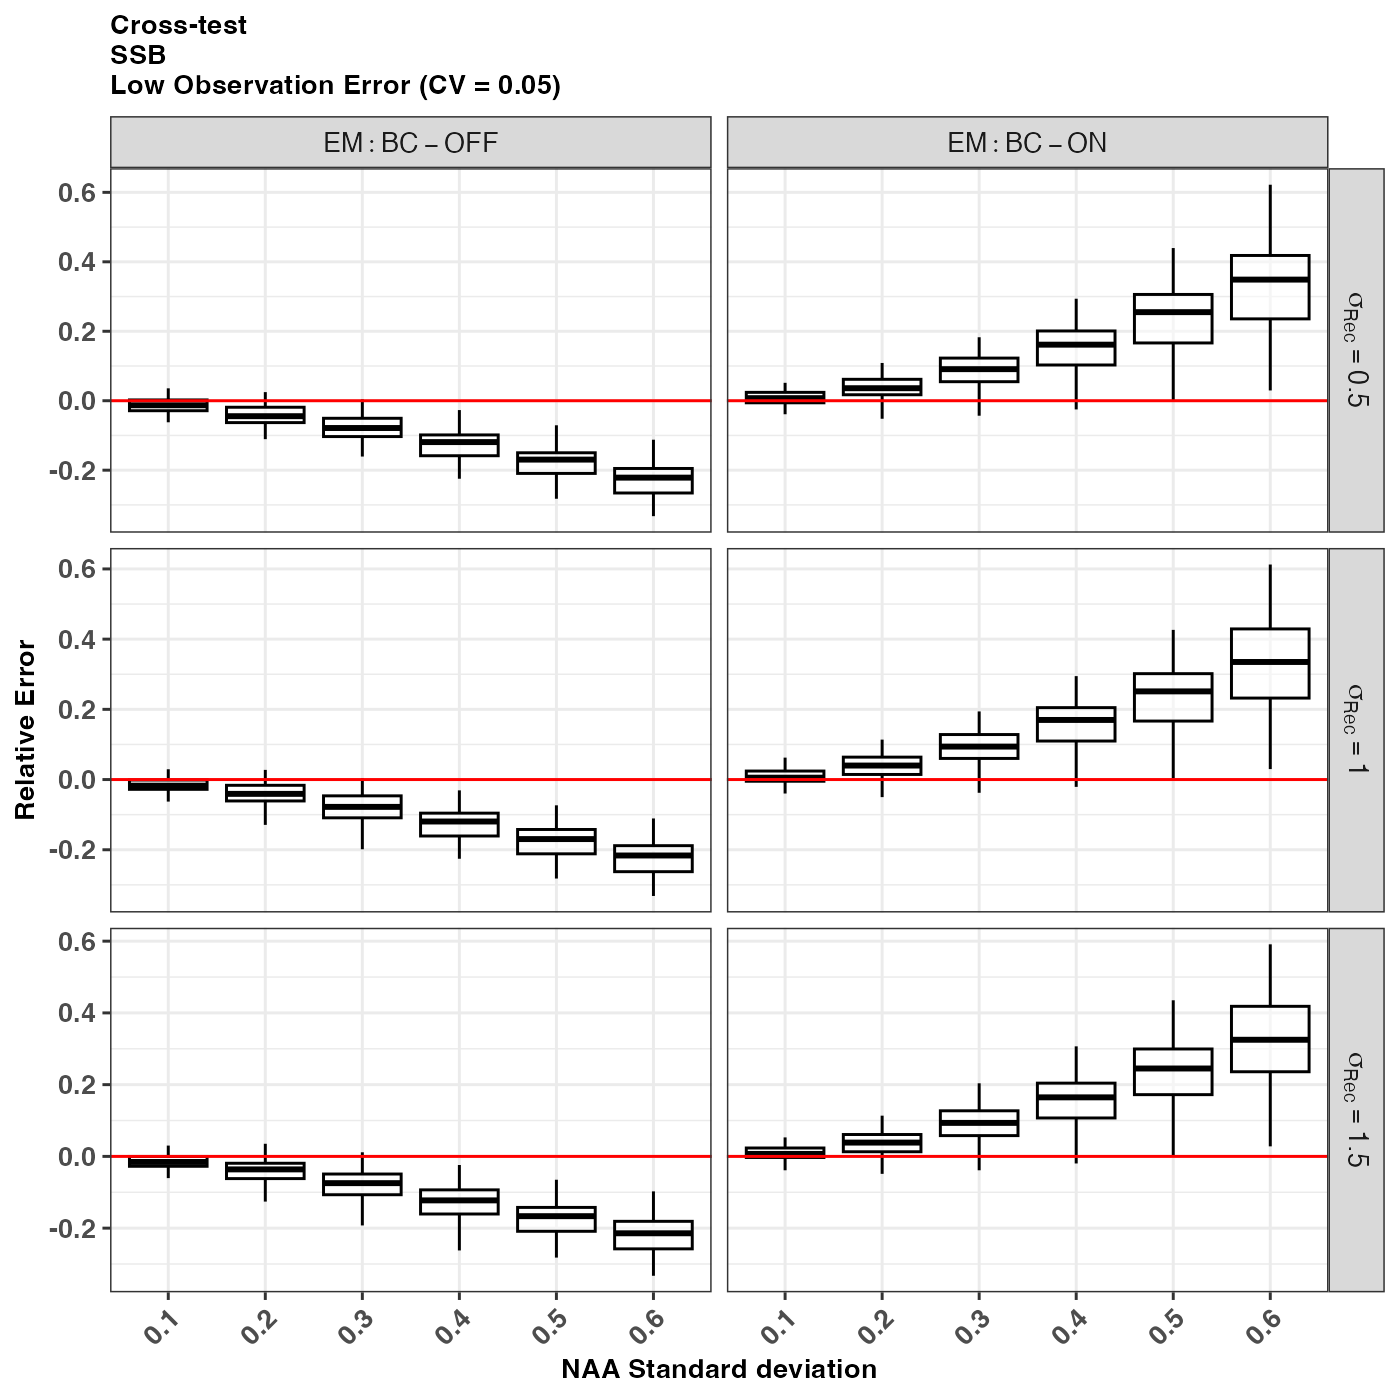
\includegraphics[width=\textwidth]{Revised_Figures&Tables/SSB_low_cross_RE.PNG}
\caption{Relative errors of $SSB$ estimates summarized from 50 realizations for each scenario. Two operating models (OMs) (with bias correction applied or omitted for both processes and observations) for Gulf of Maine (GoM) haddock with both recruitment and $NAA$ IID random effects (see Table S2) were used to conduct simulation-estimation experiments. The study evaluated the effects of recruitment variability ($\sigma_{Rec}$ = 0.5, 1, 1.5) and $NAA$ variability ($\sigma_{NAA}$ = 0.1, 0.2, ... 0.6) in a factorial design through self-tests and cross-tests. To isolate the impact of observation error, the coefficient of variation (CV) for observations was set to 0.05.}
\label{fig:supp_SSB_low_cross_RE} 
\end{figure}

\begin{figure}[H]
\centering
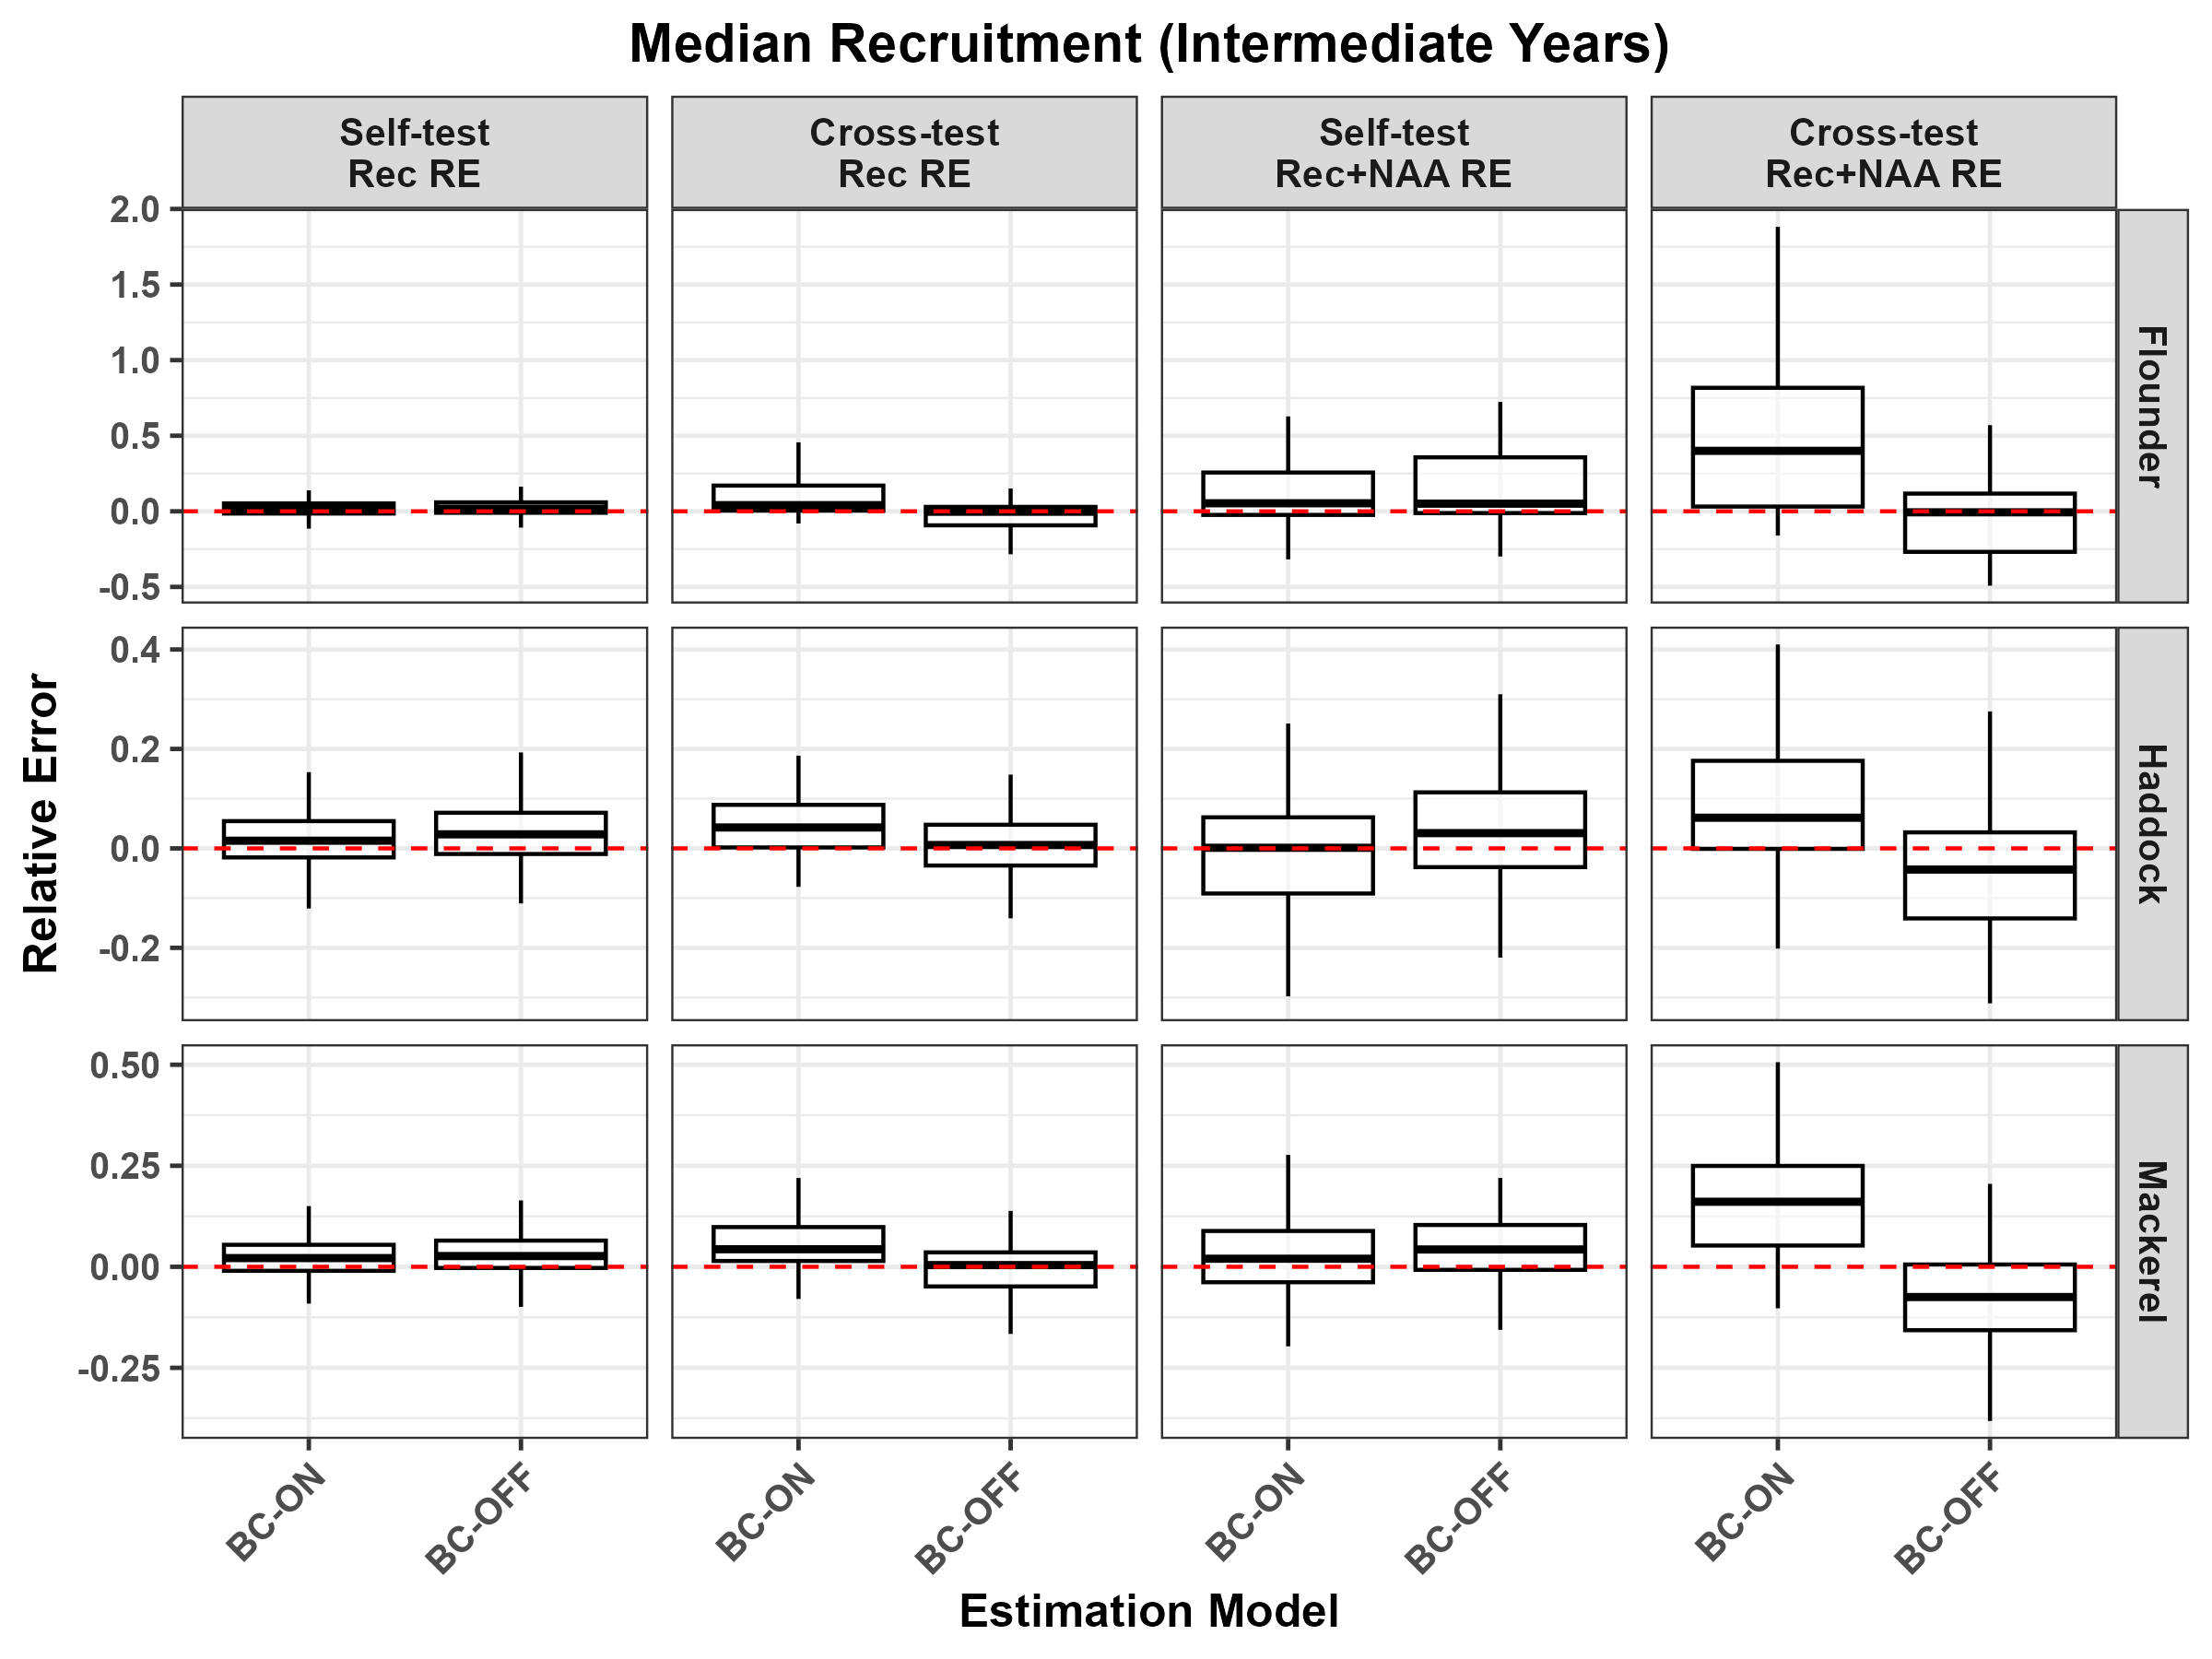
\includegraphics[width=\textwidth]{Revised_Figures&Tables/Rec_intermediate.PNG}
\caption{Median relative error of recruitment in the intermediate period (with first and last 10 years of estimates removed).}
\label{fig:supp_Rec_intermediate}
\end{figure}

\begin{figure}[H]
\centering
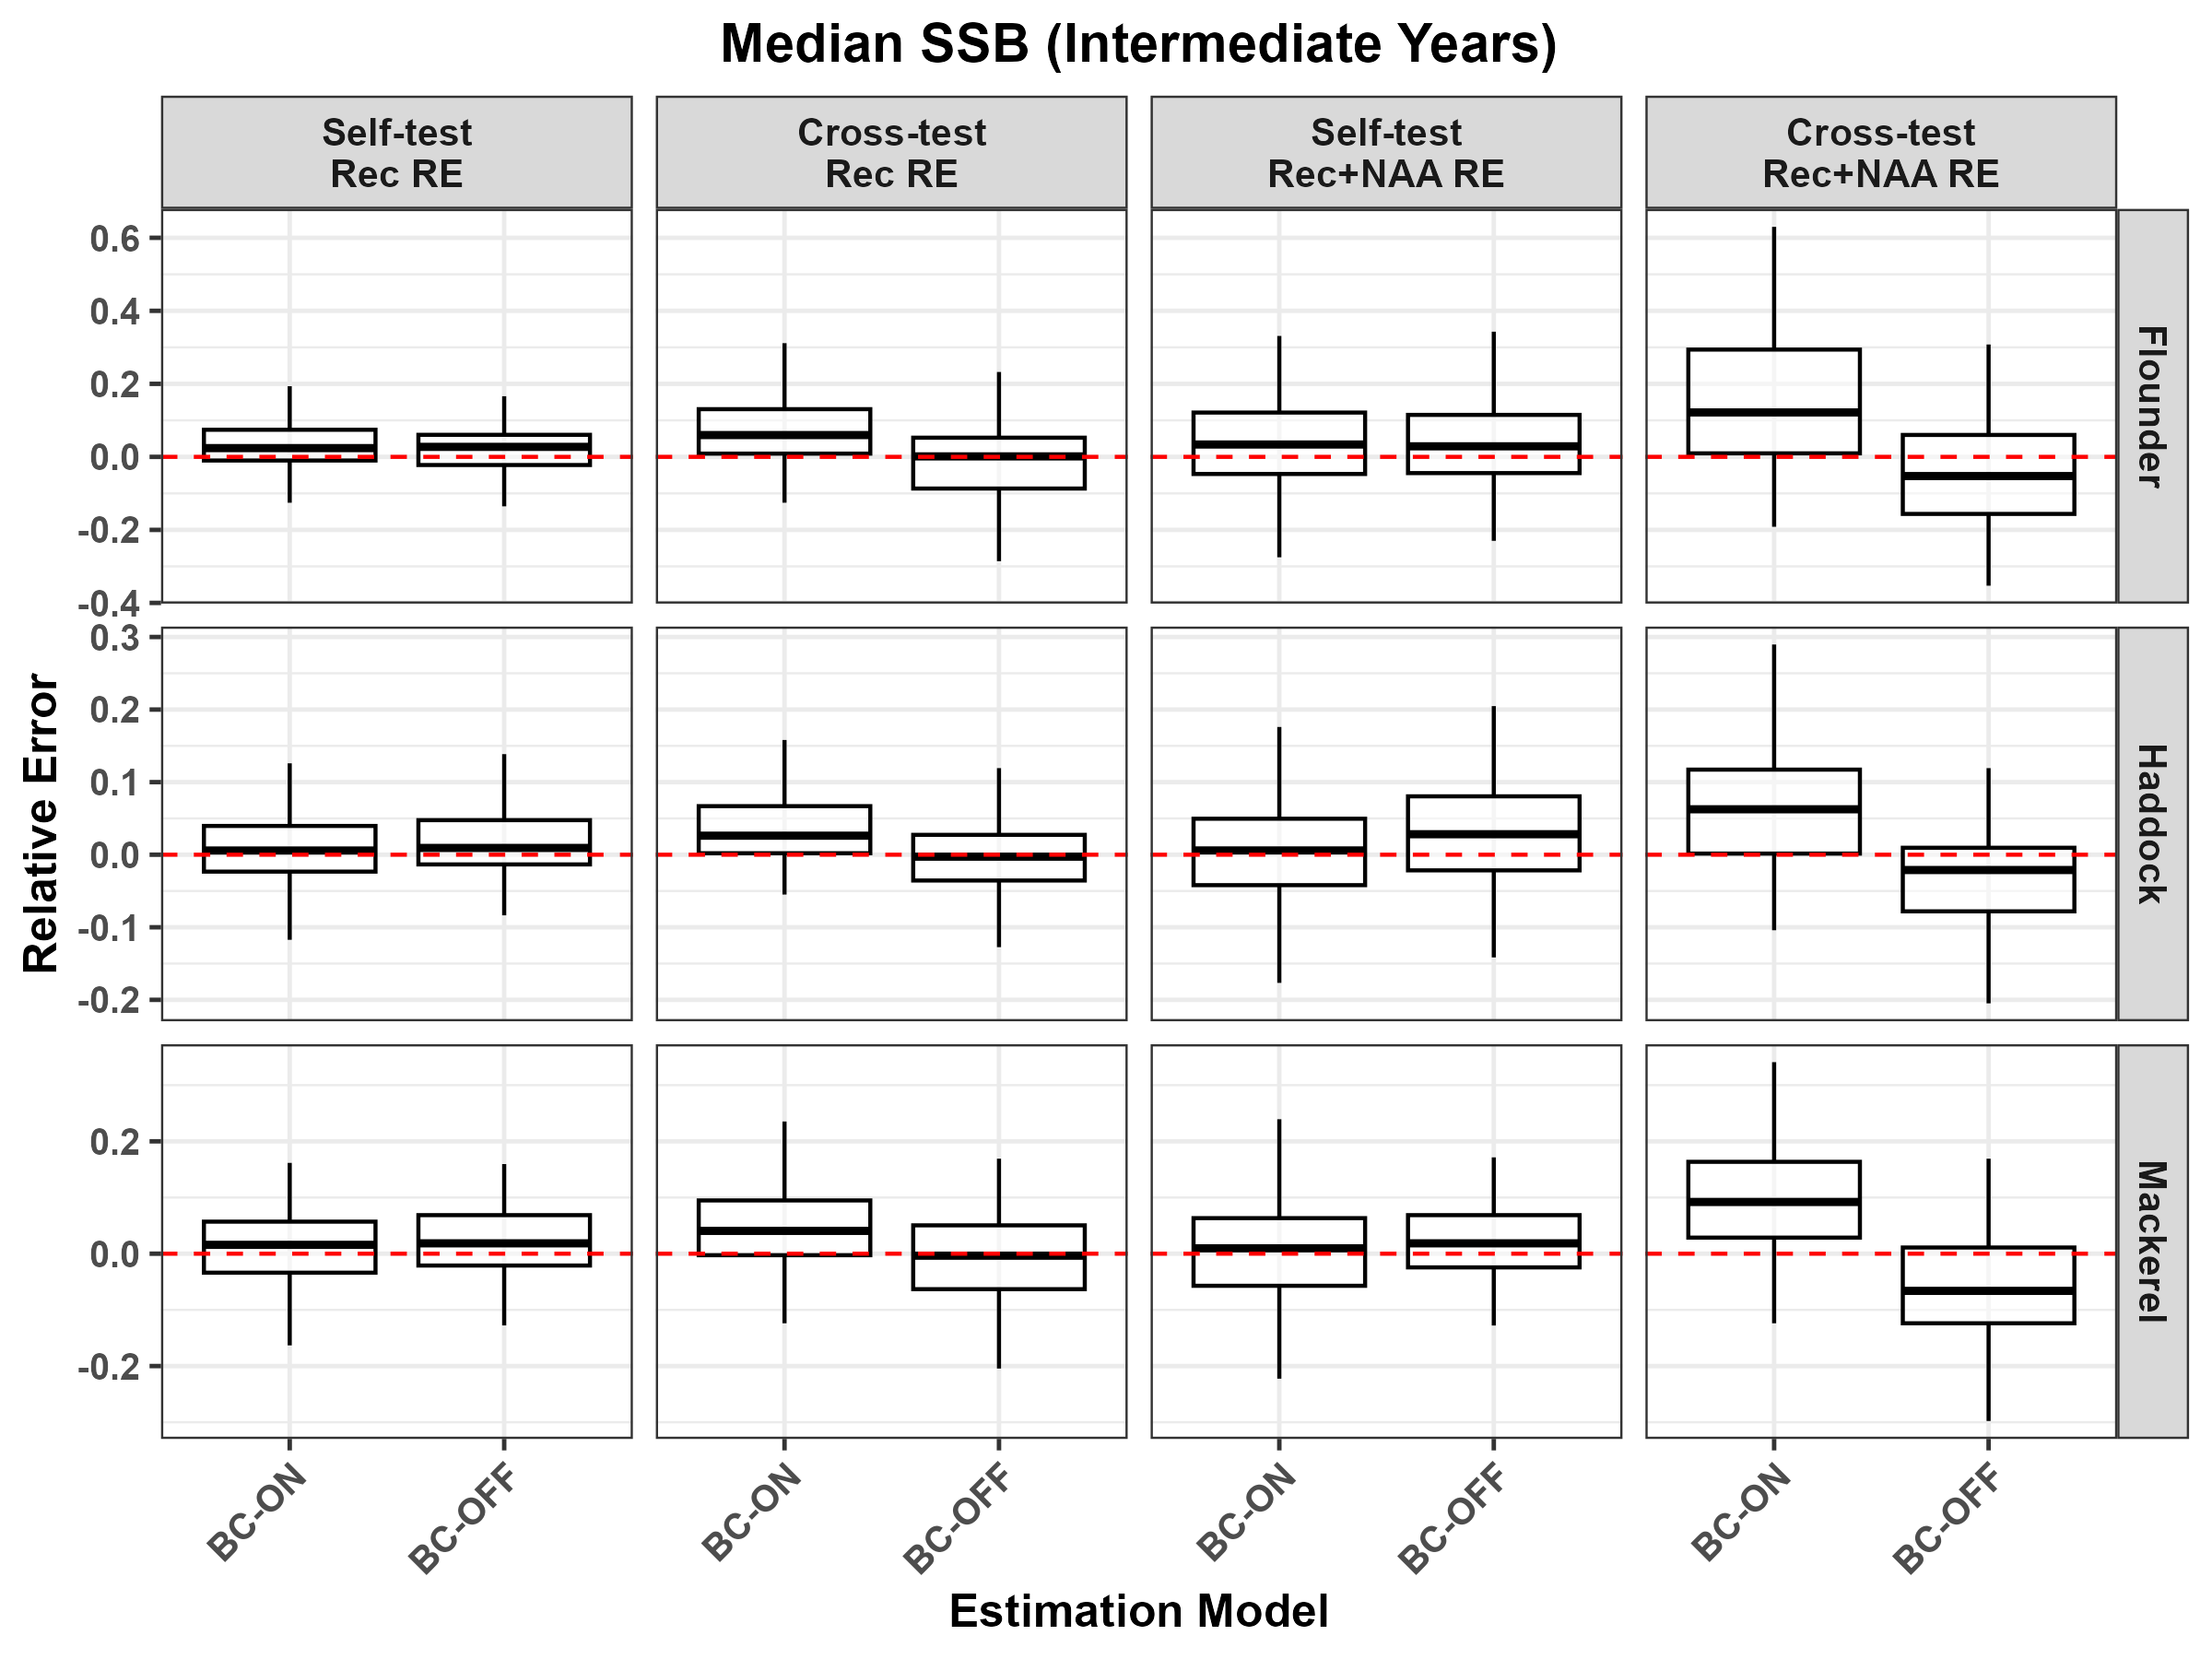
\includegraphics[width=\textwidth]{Revised_Figures&Tables/SSB_intermediate.PNG}
\caption{Median relative error of $SSB$ in the intermediate period (with first and last 10 years of estimates removed).}
\label{fig:supp_SSB_intermediate}
\end{figure}

\renewcommand{\thefigure}{\arabic{figure}}

\end{document}
